\documentclass{FastFyp}

% --- Packages (preamble) ---
\usepackage{placeins}
\usepackage{float}
\usepackage{fancyhdr} % headers/footers

\begin{document}
\newcommand{\supervisor}{Maryam Nasim}
\newcommand{\university}{National University of Computer and Emerging Sciences, Lahore}
\newcommand{\fyptitle}{Growise: AI-Powered Dynamic Learning Platform}
\newcommand{\degree}{BS (Data Science)}
\newcommand{\Studentone}{Muhammad Umair Imran     22L-8370    BS(DS)} 
\newcommand{\Studenttwo}{Muhammad Shahzad Waris     22L-7530    BS(DS)}
\newcommand{\Studentthree}{Ameer Tufail     22L-7530    BS(DS)}
\date{\today}

\renewcommand{\contentsname}{Table of Contents}

\makeatletter
    \begin{titlepage}
        
\includegraphics[width=0.2\linewidth]{Figures/nulogo.png}\hfill
        
\includegraphics[width=0.2\linewidth]{Figures/fast.png}\\
        \begin{center} 
            {\large\bfseries \university}\\[7ex]
            
\includegraphics[width=0.4\linewidth]{Figures/fastlogo.png}\\[8ex]
            {\huge \bfseries  \fyptitle }\\[10ex] 
            {\Studentone}\\{\Studenttwo}\\{\Studentthree}\\[4ex] 
            {Supervisor: \supervisor} \\ [10ex]
            {Final Year Project}\\
            {\large \@date}
        \end{center}
    \end{titlepage}    
\makeatother
\frontmatter

\newpage \thispagestyle{empty} \mbox{} \newpage %Aatira

\pagestyle{empty}  %Aatira
\section*{\begin{center}{Anti-Plagiarism Declaration} \end{center}} %Aatira
This is to declare that the above publication was produced under the:
\begin{flushleft}
\bf Title: \fyptitle
\end{flushleft}

is the sole contribution of the author(s), and no part hereof has been reproduced as it is the basis (cut and paste) that can be considered Plagiarism. All referenced parts have been used to argue the idea and cited properly. I/We will be responsible and liable for any consequence if a violation of this declaration is determined.
\\[4ex]
%% FYPTODO add the date and your names here
Date: 14/10/2025
\begin{flushright}

Name: Muhammad Umair Imran\\[1ex]

\includegraphics[width=4cm]{Figures/umair signature.png}\\[4ex]

Name: Muhammad Shahzad Waris\\[1ex]

\includegraphics[width=4cm]{Figures/shahzad signature.png}\\[4ex]

Name: Ameer Tufail\\[1ex]

\includegraphics[width=4cm]{Figures/ameer signature.png}\\[4ex]


\end{flushright}


\vspace{5 cm} %Aatira
 
\hrule %Aatira

\section*{Author's Declaration}
This states Authors’ declaration that the work presented in the report is their own, and has not been submitted/presented previously to any other institution or organization.
\pagebreak  

\section*{Abstract}

This project gives a smart learning platform for programmers. It helps them get real problem-solving skills. It does not let them only remember code without thinking. The system first looks at what the learner knows now and his technical past. Then it makes a personal learning road that fits only him. During all the learning time, an AI helper gives help right away, explains things, and brings good materials to make understanding better. After every small part, learners get tested with real coding work that is same as what big company engineers do every day. By mixing learning that changes for each person, non-stop feedback, and real hand practice, the platform helps learners grow true programming power and makes them much more ready for real jobs in software making.

\pagebreak
\section*{Executive Summary}
Today tech world change very very fast. Developer must learn new tool and new way super quick. But old school programming course not good. They only make student remember code word and follow same long plan for everybody. This waste time a lot because some people already know some thing and some want different job. This old way make people not ready for job and they feel bored and stop learn.

So we make one smart learning platform. It teach you how to think like real programmer and how to solve problem, not just remember code like robot. First day the platform give you small test. It check what you know already and what you good at. Then it ask you want learn web or AI or what. After that it make one special plan only for you. You only study what you really need. No waste time.

All the time you study, one AI teacher stay with you. It explain hard thing with easy word. It answer your question fast. It give you video or article that help you right now. After each lesson, you complete projects that feel like real work situations. These projects test whether you understand the concepts and can make good decisions about how to solve problems. You can track your progress on a dashboard that shows you what you're good at, what you need to work on, and how to improve.

By moving away from long, one-size-fits-all courses to a flexible, problem-solving focused approach, this platform bridges the gap between school and real jobs. It helps you grow faster as a developer, teaches you how to think through problems step by step, and gives you skills you can actually use at work. The platform keeps up with how modern software development actually works.
\pagebreak


\pagestyle{fancy} %Aatira
% ----- FRONT MATTER LISTS (no headers) -----
\pagestyle{empty}
\renewcommand{\contentsname}{Table of Contents}
\tableofcontents

\listoffigures
\addcontentsline{toc}{chapter}{List of Figures}

\listoftables
\addcontentsline{toc}{chapter}{List of Tables}

% ----- START MAIN MATTER + ENABLE HEADERS -----
\mainmatter

\pagestyle{fancy}
\fancyhf{}                % clear header/footer
\fancyhead[L]{\leftmark}  % left: current chapter title
\fancyhead[R]{\thepage}   % right: page number
\renewcommand{\headrulewidth}{0.4pt}

\chapter{Introduction}

Software development has shifted quickly since ChatGPT came out in 2022. Developers now have to pick up new tools and frameworks on a regular basis just to keep their work relevant. Traditional coding courses move too slowly for this kind of pace. They follow fixed schedules and lesson plans that were set months or years ago.

We built this project to close that gap. The platform starts by testing what a learner already knows, then builds a study plan around their gaps and goals. An AI mentor stays with the learner through each lesson and offers feedback as they work. The assessments we include are designed to feel closer to what a junior developer would face on the job. We want learners to understand the concepts well enough to apply them, not just recall them. The rest of this report walks through how we designed the system, how we built it, how we tested it, and what we found.

\section{Purpose of this Document}

This document describes how we designed, built, and tested a learning platform aimed at programmers. We set out to make the learning process faster, more personal, and more focused on problem solving instead of memorization. Most online courses give every learner the same fixed content. Our approach starts with an assessment and then shapes the roadmap around the learner's current level and the career path they want to follow. The question we kept coming back to is whether an AI-driven system can make learning genuinely personal and help developers move through material faster by focusing on how they solve problems. The platform we built tries to answer that. It assesses skills, offers a personalized AI mentor, and reviews code the way a senior developer might. This document covers the research we did, the design decisions we made, how we built the system, what we tested, what worked, what did not, and what we plan to do next.


\section{Intended Audience}

We wrote this report for two groups. The first is the academic side: supervisors, examiners, and faculty who need to assess the project on its technical merit and originality. The second is the practical side: new developers, self-taught coders, and anyone trying to learn programming faster without giving up depth. We kept the technical sections detailed enough for the academic review and wrote the explanations clearly enough that a working programmer can read them and take something useful away.


\section{Definitions, Acronyms, and Abbreviations}
List Of Abbreviations:  
SDG: Sustainable Development Goal\\
FYP: Final Year Project\\
MVP: Minimum Viable Product\\
UI: User Interface\\
UX: User Experience\\
Agile: Agile Development\\
SCRUM: Scrum Development\\
REST: Representational State Transfer\\
ORM: Object-Relational Mapping\\
CRUD: Create, Read, Update, Delete\\
API: Application Programming Interface

\section{Conclusion}

GrowWise is our attempt at a more personal way to learn programming. It builds a plan around each learner, keeps an AI mentor on hand, and sets projects that feel closer to real engineering work. The problem we want to solve is that most traditional courses train people to memorize syntax rather than think through problems. This report explains the core idea, the requirements we pulled together, and the system design we arrived at. What we have now is a solid foundation. We still have work left. We plan to keep building on this during FYP-2 until GrowWise reaches a complete, production-ready state.



\chapter{Project Vision}

This chapter covers the thinking behind the platform. We go over what we think is broken in how programming is taught today, what we want to fix, the goals we set for the project, and the boundaries of what we chose to build. By the end of this chapter, readers should understand why we started this project and how we believe it can change the way programmers learn.

\section{Problem Domain Overview}
We started GrowWise because most programming courses treat every learner the same way. The lessons rarely adjust to a learner's current skill or the way they think. That kind of rigidity slows people down. Learners often end up spending time on material they already understand, and when they do reach gaps in their knowledge, the course is not designed to notice.

The tech industry moves faster than curricula can keep up with. Developers need to learn how to approach problems, not just repeat syntax. Most platforms still measure success by whether a learner can memorize a snippet or follow a tutorial. They rarely push learners to compare approaches or understand why a design choice works.

We want to fix this with AI. The system starts with an assessment, then shapes a personal path around the learner. The point is to avoid wasted time, build actual problem-solving skills, and get the learner closer to what a working developer needs to know.

\section{Problem Statement}

Most learning platforms move slowly and treat every learner identically. They do not consider current skill levels or how individuals approach problems. Developers need a form of teaching that helps them learn to reason through problems rather than memorize tools and frameworks.

\section{Problem Elaboration}

Current learning platforms have several overlapping issues that make it harder for new developers to become job-ready. The main problems we want to address:

\begin{enumerate}
  \item No personal plan: Most platforms hand the same lesson to every learner, regardless of background or goals. Learners get bored or lose momentum.

  \item Wrong starting level: Courses rarely check what a learner already knows. Time gets spent on familiar material, or learners get thrown into something too advanced.

  \item Long and rigid courses: Traditional courses run for weeks or months. By the time they finish, the tools have changed.

  \item Focus on memorization: Most courses teach syntax, not reasoning. When a new tool appears, learners are back where they started.

  \item Shallow practice: Real learning happens when someone builds something real. Most platforms offer small, isolated exercises instead.
\end{enumerate}

\section{Goals and Objectives}

Our main goal is to build a learning platform that teaches developers how to think through problems, not just how to write code. We want to give learners a faster, more personal experience with AI assistance available whenever they need it.

The specific objectives:

\begin{enumerate}
    \item Personal study plan: The system begins with an assessment and then creates a plan based on the learner's strengths, weaknesses, and career goals.

    \item Right starting point: The learner begins at a level that matches their current skills. No time wasted on the basics if they already know them, and no frustration from jumping straight into advanced material.

    \item Flexible pacing: Lessons are short and responsive. If a learner moves quickly, the path adjusts. If they struggle, the path slows down.

    \item Reasoning over recall: We focus on teaching engineering thinking, including logic, trade-offs, and system design.

    \item Realistic projects: Assignments are closer to what a developer would see at a company. No trivial exercises.

    \item Responsive AI mentor: The mentor works like a patient senior engineer. It points to relevant videos or articles, answers questions, and helps when the learner gets stuck.
\end{enumerate}

\section{Project Scope}
This project is a learning platform for developers. It adjusts the lessons for every learner based on their current skill level, learning speed, and career goals such as web development, AI, or security. From there, it delivers only the content that matters for that path. We wanted the platform to go beyond traditional courses by adding AI mentorship, thorough skill assessments, and a focus on problem-solving methods.

The platform enables users to:
\begin{itemize}
    \item Register and log in through a secure authentication flow.
    \item Take an initial test that covers both technical knowledge and problem-solving ability.
    \item Choose a specialization such as web development, AI, or cybersecurity.
    \item Receive a custom learning plan based on the test results and the chosen specialization.
    \item Work with an AI mentor that explains concepts, gives feedback on code, and suggests relevant videos or articles as the learner progresses.
    \item Complete realistic project assignments that check both problem-solving and system design skills.
    \item Track their own progress on a personal dashboard that shows strengths, weaknesses, and what to focus on next.

  \end{itemize}

We built the platform on FastAPI for the backend, React.js for the frontend, and Python for the AI components. The AI mentor uses retrieval-augmented generation to pull relevant content and answer learner questions. We followed an Agile workflow with short iterations, frequent testing, early bug fixes, and steady feedback from users.

What the project delivers:
\begin{itemize}
    \item A working web application that runs in a browser and provides the personalized AI learning experience.
    \item A full report covering how the system works, the choices behind it, the implementation, and the testing.
    \item A user guide that walks learners through the platform step by step.
\end{itemize}

What the project does not include:
\begin{itemize}
    \item Integration with external learning management systems.
    \item A mobile application for Android or iOS.
    \item A large-scale deployment for thousands of concurrent users. A small test server is enough for this stage.
\end{itemize}

Setting these boundaries early gave us a clear build target and a realistic finish line.

\section{Sustainable Development Goal (SDG)}

GrowWise lines up with UN SDG 4, Quality Education. The goal calls for inclusive, equitable education and lifelong learning for everyone. We support this by using AI to tailor lessons to each learner. Learners who move fast and learners who move slowly get the same attention from the platform. Fast feedback, realistic project work, and current industry topics help users build the skills employers are actually looking for. Because the platform is open to anyone with a browser and can be used on the learner's own schedule, it lowers the barrier for people who cannot afford expensive courses or keep to a fixed class timetable. That is how GrowWise contributes to SDG 4. \ref{fig:sdg_quality_education}.

\begin{figure}[H]
    \centering
    
\includegraphics[width=0.5\textwidth]{Figures/Picture3}
    \caption{SDG 4 Quality Education, the goal GrowWise aligns with.}
    \label{fig:sdg_quality_education}
\end{figure}

\section{Constraints}

Building this platform came with several constraints that shaped our decisions:

\begin{itemize}
    \item Hardware limits: RAG-based AI and mentor models need significant memory and compute. Our development hardware struggles with heavier workloads and occasionally slows down or crashes.

    \item Limited time: This is a final year project, so we had only a few months. We could not build out every idea we had or add highly advanced capabilities.

    \item Integration complexity: The assessment AI, mentor AI, and chat interface need to work together smoothly, and coordinating them has introduced bugs along the way.

    \item Internet dependency: All AI features and content retrieval require a network connection. Without one, the platform cannot function.

    \item Small user base for now: This version targets a small test group. A production deployment with thousands of simultaneous users is a later concern.
\end{itemize}

\section{Business Opportunity}
GrowWise is more than a learning app. It also has a clear commercial angle. Individuals, companies, and schools all have reasons to pay for a platform like this. Traditional courses rarely offer personal pacing or real problem-solving training. GrowWise offers both, and that gives it a distinct position in the market. Many programmers want to gain strong skills quickly, and many companies need to onboard developers fast. Both groups are reasonable customer targets, and both can support a healthy business model.

\section{Stakeholders Description/ User Characteristics}

This section describes who the platform is built for and what they need from it. We spent time understanding both groups so the platform would actually serve them.

\subsection{Stakeholders Summary}

GrowWise is built for two main audiences:

\begin{itemize}
    \item Developers and junior programmers: This is the primary audience. They range from students and career switchers to self-taught coders and junior developers looking to level up. They want a platform that matches their skill level, adjusts its pace as they learn, and teaches them how to think about problems rather than memorize solutions. The end goal is to get them ready for actual engineering work.

    \item Tech companies and teams: Larger companies and smaller engineering teams that need to train developers efficiently. They want visibility into who is progressing, scalable training for multiple people at once, and assurance that trainees can handle real projects. Progress reports and certificates are useful to them.
\end{itemize}

\subsection{High-Level Goals and Problems of Stakeholders}

\begin{itemize}
    \item Junior programmers: Want a personal learning plan, practical problem-solving experience, and lessons that avoid rote memorization.

    \item Companies: Want their developers to learn quickly, want clear progress tracking, and want their people to be ready for real work without a long onboarding period.
\end{itemize}

Understanding what each group needs helps us make design decisions that serve both without compromising either.
\section{Conclusion}

This chapter laid out the core idea behind GrowWise. We covered the problems with traditional programming courses and why they matter, the goals we set for ourselves, and the line between what we planned to build and what we had to leave out given our timeline. We also touched on the commercial case for the platform. With all of that on the table, the next chapter moves into how we designed and built the system.
\chapter{Literature Review / Related Work}

This chapter covers the tools and platforms we looked at while designing GrowWise. We studied systems that handle personalized learning, project-based practice, or AI-assisted programming instruction. Each one gave us something useful. GrowWise takes what we found most effective from these systems and adds RAG-based knowledge retrieval, AI-driven code review, and a personalized learning plan aimed at junior developers who want to build practical engineering skills.
\section{Definitions, Acronyms, and Abbreviations}

This section clarifies the short forms and specialized terms used in this chapter.

\subsection{Key Definitions}

Adaptive Learning: An approach that adjusts lesson content, pacing, and delivery style based on how the learner progresses.

Agentic AI: AI that can plan and carry out tasks on its own, without needing step-by-step instructions from a user.

Approach-Oriented Learning: Teaching that focuses on how to think about a problem rather than on memorizing specific code.

Learning Path: A sequence of study materials, exercises, and assessments arranged to help a learner reach a goal.

Micro-Learning: Short, focused lessons, usually just a few minutes each, designed to fit into busy schedules.

Personalized Learning: Instruction shaped around an individual learner's pace, interests, and skill level.

RAG (Retrieval-Augmented Generation): An AI technique where the model first searches a knowledge base, then generates an answer grounded in what it found.

Skill Assessment: A test that measures what a learner currently knows and where the gaps are.


\section{Detailed Literature Review}
This section reviews the platforms that inspired GrowWise. We looked at each one carefully and examined how it relates to the work we are doing.




\subsection{Crio.Do}

\subsubsection{Summary}
Crio.Do \cite{ref:CrioDo:2025} is an online learning platform designed to bridge the gap between academic programming and actual industry work. It partners with companies such as CRED and assigns learners real projects that match what engineering teams actually build. The focus is on doing, not theorizing. Students and junior developers typically finish with a portfolio of production-style work and a strong base for job applications.

\subsubsection{Critical Analysis (Strengths and Weaknesses)}
Strengths: Offers hands-on experience with projects that mirror industry work. Its partnerships with real companies lend it credibility and align the curriculum with what employers want.
Weaknesses: Its tech coverage is limited. Beginners can find the projects too difficult. The time commitment is significant, and working learners often struggle to finish.

\subsubsection{Relationship to Proposed Work}
We took inspiration from Crio.Do's project-based approach. Our platform goes further by using AI to generate personal learning plans for every user, adjusting content as learners progress, and covering a broader set of technologies.


\subsection{The Odin Project}

\subsubsection{Summary}
The Odin Project \cite{ref:TheOdinProject} is a free, open-source curriculum that teaches full-stack web development. It covers HTML, CSS, JavaScript, Git, Node.js, databases, and more, taking learners from beginner to job-ready. Instead of step-by-step video tutorials, it pushes learners to build their own applications, which forces them to develop problem-solving skills along the way. The whole curriculum is free, and a community supports learners along the way. It works well for self-directed people aiming at a web development career.

\subsubsection{Critical Analysis (Strengths and Weaknesses)}
Strengths: Fully free, well-ordered curriculum, and a large community for support.
Weaknesses: Heavy self-direction means less motivated learners often drop off. The material is mostly text, which limits interactivity. The exercises do not feel like industry work.

\subsubsection{Relationship to Proposed Work}
Like The Odin Project, we emphasize learning through building. Our platform adds an AI mentor that gives personalized help, adjusts the path based on progress, and delivers fast feedback as learners work.
\subsection{ProjectLearn.io}

\subsubsection{Summary}
ProjectLearn.io \cite{ref:ProjectLearn} is a platform that teaches programming through complete application projects. It offers tutorials for web, mobile, game development, and machine learning. Instead of small exercises, learners build full applications from scratch and see how the parts fit together. Tutorials are grouped by technology and difficulty level, which makes it easy to pick one that matches a learner's current abilities. The platform works well for students who want tangible portfolio pieces rather than pure theory.

\subsubsection{Critical Analysis (Strengths and Weaknesses)}
Strengths: A wide range of projects across several domains. It helps learners build a portfolio and offers content at multiple difficulty levels.
Weaknesses: Tutorial quality varies because content comes from many contributors. There is no personalized plan, and the platform does not offer much interactivity beyond the projects themselves.

\subsubsection{Relationship to Proposed Work}
GrowWise shares the project-based philosophy but adds better structure and personalization. Our AI adjusts the path for each learner and delivers faster feedback throughout.

\subsection{Educative.io}

\subsubsection{Summary}
Educative.io \cite{ref:Educative} targets developers who already know the basics. It covers advanced topics like system design, interview preparation, backend engineering, and topics commonly asked about at larger tech companies. Its strongest feature is the in-browser coding environment, which removes the setup friction. Its AI tracks progress and provides personalized paths along with quick feedback. It works well for mid-level developers preparing for interviews.

\subsubsection{Critical Analysis (Strengths and Weaknesses)}
Strengths: In-browser coding removes setup hassle. Strong catalog for interview and system design topics. AI builds personalized paths.
Weaknesses: A subscription is required for most content. Full-stack fundamentals are underrepresented. Absolute beginners may find it too advanced.

\subsubsection{Relationship to Proposed Work}
We borrow the in-browser coding and AI-personalization ideas from Educative.io. Our platform focuses more on beginners and junior developers and offers a full path from the start, with more active AI support along the way.


\subsection{Codio}

\subsubsection{Summary}
Codio \cite{ref:Codio} is a cloud-based learning platform that offers real coding environments inside the browser. Its courses cover AI, data, security, and full-stack development. The standout feature is that learners use the same tooling as working engineers, including GitHub and CI/CD pipelines. There is no local setup required, which makes it popular with schools and corporate training programs that need to get learners productive quickly.

\subsubsection{Critical Analysis (Strengths and Weaknesses)}
Strengths: Industry-standard tooling with no setup. A varied catalog of courses.
Weaknesses: Beginners can feel overwhelmed by the tooling. A subscription is required for serious use. The community around it is smaller, so peer support is limited.

\subsubsection{Relationship to Proposed Work}
Like Codio, we offer a real coding environment. Our platform aims to be more beginner-friendly, with AI-driven personalization, responsive help, and a pace that avoids overwhelming new developers.


\subsection{Project-Based Learning GitHub Repository}

\subsubsection{Summary}
This GitHub repository \cite{ref:GitHubProjectBasedLearning} is a community-maintained collection of project tutorials across many stacks: web, mobile, data science, and a wide range of languages. The list is organized by language, which makes it easy to browse. Learners build full applications from scratch and end up with portfolio-worthy work. It fits independent learners who do not need a guided curriculum or active mentorship.

\subsubsection{Critical Analysis (Strengths and Weaknesses)}
Strengths: Free, a large catalog of projects across many languages, and useful for portfolio building.
Weaknesses: No structured learning path, which makes it easy for beginners to get lost. Tutorial quality varies widely. Everything is text-based, with no integrated coding environment or quick help when learners get stuck.

\subsubsection{Relationship to Proposed Work}
We share the project-based approach but provide structure the repository lacks. Our platform offers a clear step-by-step plan, an AI mentor that is always available, personal pacing, and projects that grow in difficulty as learners improve. This keeps learners from getting stuck or losing direction.




\subsection{Udemy}

\subsubsection{Summary}
Udemy \cite{ref:Udemy} is a large online course marketplace with more than 200,000 courses across programming, web development, data science, and many other fields. Any instructor can publish and sell a course. The content is mostly video-based, with some downloadable files and occasional coding exercises. Courses are inexpensive and can be taken at the learner's own pace. It serves beginners and experienced developers alike, though course quality is inconsistent.

\subsubsection{Critical Analysis (Strengths and Weaknesses)}
Strengths: A huge catalog, low prices, flexible pacing, and ratings that help learners choose.
Weaknesses: Courses are static and offer no personalization. Feedback is almost non-existent. Many courses are passive video-watching with limited hands-on work. Completion rates are low because nothing pushes learners to finish.

\subsubsection{Relationship to Proposed Work}
Udemy's strengths lie in catalog size and affordability. Our platform improves on the experience with AI-generated plans, quick feedback, hands-on projects, and a responsive AI mentor. The focus is on thinking and problem-solving, not watching videos and forgetting them later.

\subsection{LinkedIn Learning}

\subsubsection{Summary}
LinkedIn Learning \cite{ref:LinkedInLearning} is a video-based learning platform aimed at working professionals. It covers technology, business, and creative skills. The tight LinkedIn integration is its most useful feature: completed courses appear as certificates on a learner's profile, which hiring managers can see directly. Course recommendations are based on the learner's job title and skills. Instructors are typically industry professionals. It suits workers who want to present new skills to employers and progress in their careers.

\subsubsection{Critical Analysis (Strengths and Weaknesses)}
Strengths: Solid video quality, LinkedIn-integrated certificates, career-aligned recommendations, and clear career tracks.
Weaknesses: Mostly video-based with little hands-on coding or project work. Personalization is shallow. No rigorous assessments that mirror actual engineering work.

\subsubsection{Relationship to Proposed Work}
We took the career-alignment idea from LinkedIn Learning. Our platform goes further for programmers specifically: an always-available AI mentor, realistic projects, quick feedback, and a learning path that adjusts continuously. The aim is actual capability, not just a certificate on a profile.

\subsection{Microsoft Learn}

\subsubsection{Summary}
Microsoft Learn \cite{ref:MicrosoftLearn} is a free platform from Microsoft that covers Azure, Microsoft 365, the Power Platform, and other Microsoft products. Learners can work with real cloud tools in a sandbox environment at no cost. It offers clear career tracks, including developer and administrator paths, along with recommendations based on what the learner has completed. Everything is free and includes labs, interactive tutorials, and short assessments. It works well for anyone planning to work with Microsoft technology.

\subsubsection{Critical Analysis (Strengths and Weaknesses)}
Strengths: Free, real Microsoft tooling in sandboxes, well-structured learning paths, and some personalization.
Weaknesses: Limited to Microsoft technologies. The exercises are mostly small, not full projects. The assessments measure task completion rather than reasoning or system design.

\subsubsection{Relationship to Proposed Work}
We drew inspiration from Microsoft Learn's personalized recommendations and free lab access. Our platform is not tied to any single vendor and covers a broader set of technologies. The focus is on problem-solving, reasoning, system design, and substantial project work. The AI mentor supports learners at every step with specific, context-aware guidance.


\subsection{Pluralsight}

\subsubsection{Summary}
Pluralsight \cite{pluralsight2023} is a subscription-based learning platform aimed at IT professionals and developers. Its library covers thousands of video courses on programming, cloud, security, and related topics. The Skill IQ assessment is its signature feature. It measures proficiency in a technology quickly and then generates a personal plan that highlights weak areas and suggests courses. Many companies use it because it provides quantifiable skill data that simplifies team training.

\subsubsection{Critical Analysis}
Strengths: Strong assessment system, genuinely personal learning paths, a large catalog suited to enterprise training, and benchmarking against peers.
Weaknesses: Mostly video-based with limited hands-on coding. Little emphasis on reasoning, design, or large-scale problem-solving. No quick feedback on learner-written code.

\subsubsection{Relationship to Proposed Work}
Our platform and Pluralsight both begin with an assessment and personalize from there. We go beyond video by offering real projects, reasoning and design evaluation, and an AI mentor that provides specific feedback as learners work. The goal is to develop problem solvers, not course-watchers.


\subsection{CYPHER Learning (with CYPHER Agent)}

\subsubsection{Summary}
CYPHER Learning \cite{cypher2023} is an enterprise learning management system used to train large numbers of employees at once. It includes an AI called CYPHER Agent that personalizes content based on job role, current skills, and the employer's needs. The agent identifies gaps and recommends relevant courses. Large organizations use it because it simplifies training rollouts and makes completion easy to track.

\subsubsection{Critical Analysis}
Strengths: The AI personalization works well. It scales to train many people on different topics at once. It saves administrative time.
Weaknesses: It is built for general workforce training, not for developer education specifically. It does not teach software reasoning or system design. The content stays general and does not go deep on technical topics.

\subsubsection{Relationship to Proposed Work}
CYPHER demonstrates that AI-assisted personalization works at scale inside an LMS. Our platform applies a similar idea through the RAG mentor but focuses entirely on programmers. The AI delivers senior-developer-style feedback, assesses projects in depth, and teaches learners how to think about problems.


\subsection{DataCamp}

\subsubsection{Summary}
DataCamp \cite{datacamp2023} is a learning platform specialized in data science, analytics, and AI. It uses short videos followed by in-browser coding exercises, with no local installation required. Learners use Python, R, and SQL in real time. The AI adjusts difficulty based on performance and suggests courses aligned with career goals. It serves everyone from beginners to experienced practitioners in data-related roles.

\subsubsection{Critical Analysis}
Strengths: Real in-browser coding, fast feedback, adaptive AI-driven paths, and strong content for data-related work.
Weaknesses: Specializes in data science and limits itself to Python and R, leaving out web development and security. Exercises are small rather than full projects. It does not assess reasoning or system design.

\subsubsection{Relationship to Proposed Work}
Like DataCamp, our platform offers fast feedback and adapts to learners. Our scope is broader, covering more technologies, and we include larger project work that measures reasoning and design the way senior developers would evaluate code.

\subsection{freeCodeCamp}

\subsubsection{Summary}
freeCodeCamp \cite{freecodecamp2023} is a nonprofit that offers completely free programming education. The curriculum covers web development, data science, machine learning, and more. Learners build real projects, and some projects contribute to actual nonprofit organizations. Certificates are free on completion and well-regarded by employers. An AI tutor has been added recently. A large community uses the platform because it is free and the content is solid.

\subsubsection{Critical Analysis}
Strengths: Fully free, real projects, recognized certificates, AI tutor, and a large community.
Weaknesses: Mostly self-directed, so beginners can lose their way. There is no personalized plan, and nothing actively pushes learners to complete courses. Learners sometimes get stuck for long periods.

\subsubsection{Relationship to Proposed Work}
Like freeCodeCamp, we value real project work and accessible education. Our platform addresses what freeCodeCamp does not: a personalized AI-generated plan, an active AI mentor, fast feedback, and more structure to keep learners moving forward.


\subsection{Udacity}

\subsubsection{Summary}
Udacity \cite{udacity2023} offers Nanodegree programs at a premium price. The topics include AI, cloud, data science, and related fields. Content is built in partnership with large tech companies such as Google and Amazon, so it stays current and aligned with industry needs. Projects are substantial and mirror actual engineering work. Human mentors review submissions and provide feedback. Graduates are often well-positioned for senior roles, though the cost is high.

\subsubsection{Critical Analysis}
Strengths: Strong industry-aligned content, substantial projects, human mentors, and deadline structure that encourages completion.
Weaknesses: Expensive. Human mentor feedback can be slow. The learning path is largely fixed and does not adjust dynamically to learner performance.

\subsubsection{Relationship to Proposed Work}
Like Udacity, we focus on realistic projects and job readiness. Our approach replaces slow human mentor feedback with an always-available AI mentor backed by RAG, and the path adjusts as learners progress. Learners pay less and get a more personalized experience.

\subsection{CodeCombat}

\subsubsection{Summary}
CodeCombat \cite{codecombat2023} teaches programming through a fantasy game. Learners write actual Python or JavaScript to control characters and solve challenges. It works especially well for children and absolute beginners. When learners get stuck, the AI offers hints. The difficulty increases gradually as the game progresses. It makes learning the basics of code enjoyable rather than tedious.

\subsubsection{Critical Analysis}
Strengths: Engaging and game-like, which keeps learners coming back. Instant feedback and AI-driven hints keep them unstuck. A strong fit for younger learners or first-time coders.
Weaknesses: The game format does not transfer directly to real project work or system design. Problems have single correct answers, which is not how engineering work operates. Not well suited to intermediate or advanced developers.

\subsubsection{Relationship to Proposed Work}
Like CodeCombat, our platform uses AI to provide fast guidance and keep learners from getting stuck. Our focus is on working developers rather than gamified learning for beginners. We assign realistic projects and assess reasoning and design the way a senior engineer would. The goal is job readiness, not gameplay.

\section{Literature Review Summary Table}
The following table summarizes the platforms we reviewed, including their key features, their relevance to GrowWise, and the limitations we identified.

\begin{table}[!htbp]
\footnotesize
\centering
\caption{Summary of Learning Platforms Reviewed}
\label{tab:literature_summary}
\begin{tabular}{|p{2.5cm}|p{3.5cm}|p{4cm}|p{4cm}|}
\hline
Platform & Key Features & Relevance to GrowWise & Identified Limitations \\
\hline
Crio.Do \cite{ref:CrioDo:2025} & Project-based learning with real-world company projects & Provides insight into hands-on skill development and project experience & Limited to certain tech stacks; time-intensive; may overwhelm beginners \\
\hline
The Odin Project \cite{ref:TheOdinProject} & Free, open-source full-stack web development curriculum & Emphasizes learning by doing and portfolio building & Self-paced nature may reduce accountability; text-heavy; limited industry exposure \\
\hline
ProjectLearn.io \cite{ref:ProjectLearn} & Curated project tutorials across multiple domains (web, mobile, ML, game dev) & Focus on project-based learning and portfolio creation & Quality varies across creators; lacks personalized paths; limited interactive features \\
\hline
Educative.io \cite{ref:Educative} & Interactive coding courses with AI personalization & Provides hands-on coding practice and adaptive learning paths & Subscription required for some courses; limited full-stack coverage; better for intermediate learners \\
\hline
Codio \cite{ref:Codio} & Real-time coding environments with GitHub & Offers immersive, practical coding experience and workflow integration & Can be complex for beginners; subscription required; limited community support \\
\hline
Project-Based Learning GitHub Repository \cite{ref:GitHubProjectBasedLearning} & Curated tutorials for multiple languages and frameworks & Encourages learning by doing and project portfolios & Lacks structured learning paths; quality varies; limited interactivity \\
\hline
Udemy \cite{ref:Udemy} & Massive course catalog across various technologies & Wide accessibility; self-paced learning & Static content; limited personalization; minimal real-time feedback \\
\hline
LinkedIn Learning \cite{ref:LinkedInLearning} & Professional courses with LinkedIn integration & Structured career-oriented learning paths & Mostly video-based; minimal coding practice; limited project validation \\
\hline
Microsoft Learn \cite{ref:MicrosoftLearn} & Personalized learning paths with hands-on labs & Interactive exercises and adaptive recommendations & Focused on Microsoft technologies; limited assessment of problem-solving or architecture skills \\
\hline
Pluralsight \cite{pluralsight2023} & Skill IQ assessment, adaptive testing, personalized learning paths, enterprise training & Assessment-first approach, skill-level matching, industry benchmarking & Video-based delivery, limited interactive practice, focus on skill acquisition over architectural evaluation \\
\hline
CYPHER Learning \cite{cypher2023} & Agentic AI integration, adaptive learning, enterprise LMS, AI skills management & Personal learning agent validation, agentic AI philosophy, adaptive learning capabilities & Enterprise focus, generalized content, limited specialized developer training \\
\hline
DataCamp \cite{datacamp2023} & Interactive coding exercises, micro-assessments, AI-recommended paths, real-time adaptation & Interactive learning model, continuous assessment, adaptive pacing & Domain-specific focus, limited architectural reasoning, emphasis on code mastery over problem-solving approach \\
\hline
freeCodeCamp \cite{freecodecamp2023} & Free curriculum, real-world projects, community-driven learning, AI tutoring integration & Project-based learning, accessibility, real-world application & Self-paced nature, limited personalized guidance, overwhelming for beginners, lack of accountability \\
\hline
Udacity \cite{udacity2023} & Nanodegree programs, industry partnerships, project-based learning, human mentor support & Industry-ready focus, project-intensive learning, career alignment & High cost, human-gated feedback, limited scalability, fixed learning paths \\
\hline
CodeCombat \cite{codecombat2023} & Gamified learning, interactive coding, AI-driven hints, immersive environments & Engagement strategies, interactive environments, AI-driven guidance & Gamification limitations, simplified complexity, limited real-world architectural assessment \\
\hline
\end{tabular}
\end{table}

\FloatBarrier


\section{Conclusion}
In this chapter we examined a range of learning platforms: Crio.Do, The Odin Project, ProjectLearn.io, Educative.io, Codio, the GitHub project-based learning repository, Udemy, LinkedIn Learning, Microsoft Learn, Pluralsight, CYPHER Learning, DataCamp, freeCodeCamp, Udacity, and CodeCombat. These platforms emphasize learning through projects, hands-on practice, and coding exercises, which build solid skills and portfolios. Most do not offer genuinely adaptive learning that changes with the learner, AI mentors, instant feedback on conceptual understanding, or personal paths tied to current skill and career goals.

This review exposed gaps that GrowWise can fill. Our platform combines AI-driven personalization, intelligent resource retrieval, and project-based assessment to teach learners how to reason through problems. What we learned from these platforms guided the design of GrowWise. We addressed their weaknesses while strengthening learners' critical thinking, problem-solving, and practical programming skills.
\chapter{Software Requirement Specifications}
This chapter describes the main features of the project. It covers what the system should do, how it should work, the use cases it supports, and the risks we have to manage.

\section{List of Features}

The main features of GrowWise:

\begin{itemize}
    \item Secure sign-up and login with straightforward profile creation.
    \item Choice of learning track, such as AI, web development, or game development.
    \item An initial skill assessment on day one that identifies strengths and weaknesses.
    \item A personalized study plan generated from the assessment results and the chosen track.
    \item An AI mentor available during every lesson that explains concepts, offers hints, and suggests relevant videos or articles.
    \item AI-assigned realistic projects, followed by an AI-driven code review that evaluates the code, the reasoning behind it, and the design. The feedback resembles what a senior developer would give.
    \item A progress dashboard that highlights strengths, remaining gaps, and suggested next steps.
    \item Admin tools for adding new tracks, expanding the AI's knowledge base, and fixing issues when they arise.
\end{itemize}


\section{Functional Requirements}

This section lists what the system can do for each user role.

\subsection{Functional Requirements of Programmers / Developers}
Programmer users can:
\begin{itemize}
    \item Create an account and log in.
    \item Choose a track such as AI, web development, or game development.
    \item Take the initial skill assessment so the system can gauge their level.
    \item Receive a personal study plan.
    \item Work through each lesson alongside the AI mentor, with examples and video references available.
    \item Complete short exercises or mini-projects in every lesson.
    \item See progress over time along with feedback on strengths and weaknesses.
    \item Complete a final capstone project that the AI evaluates for both code and reasoning.
\end{itemize}

\subsection{Functional Requirements of Admin}
Admin users can:
\begin{itemize}
    \item Create new tracks or update existing ones.
    \item Add lessons, videos, and articles.
    \item Upload new documents into the RAG knowledge base to improve AI responses.
    \item Review user learning paths and fix issues when something goes wrong.
\end{itemize}

\subsection{Functional Requirements of System}
The system itself can:
\begin{itemize}
    \item Keep user accounts secure.
    \item Build a personalized plan for each new user.
    \item Provide AI mentor support during every lesson.
    \item Track progress and return feedback quickly.
    \item Assign major projects and evaluate submitted code with AI that mirrors senior-level review.
    \item Maintain the knowledge base so the AI has current material to draw from.
\end{itemize}

\section{Quality Attributes}

GrowWise is designed to be reliable and easy to use. The main qualities we focused on:

\begin{itemize}
    \item Reliability: The AI mentor and evaluator return accurate responses. The platform does not crash under normal load.
    \item Usability: Screens are simple and clear. Lessons, videos, and feedback are easy to find.
    \item Maintainability: The code is organized into clean, modular sections so future features and fixes are straightforward.
    \item Performance: The platform stays responsive even when several users are active at the same time.
    \item Flexibility: New tracks, knowledge sources, and features can be added without major changes.
\end{itemize}

\section{Non-Functional Requirements}

This section covers the non-functional requirements of the GrowWise platform, including performance, reliability, usability, reusability, and extensibility.

\subsection{Performance}
The system should help users learn efficiently and keep overall learning time short.

\subsection{Reliability}
The platform should be available continuously so learners can access their paths and the AI mentor without interruption.

\subsection{Usability}
The platform should be simple to use. Users should quickly understand how to navigate and follow their learning path.

\subsection{Reusability}
The code should be modular so components can be reused for new features or updates.

\subsection{Extensibility}
New learning paths, AI guidance, and project types should be easy to add over time.

\section{Assumptions}

We based the design on the following assumptions:

\begin{itemize}
    \item Users have a web browser on their computer or device that supports JavaScript.
    \item Users have an internet connection stable enough to reach the platform.
    \item Users know basic web navigation, such as clicking links and filling in forms.
    \item Users have some familiarity with programming, enough to follow the learning paths.
    \item Admins know how to create learning paths and manage the AI-driven knowledge base.
\end{itemize}

\section{Use Cases}
This section lists the use cases our application supports. The tables below document each one in detail.

% --- Use Case 1: User Login ---
\subsection{User Login}
\noindent
\begin{minipage}{\textwidth}
\centering
\captionof{table}{Use Case: User Login}
\label{tab:login}
% 5 Columns: Allows wide labels at the top (merging 1-2) and narrow IDs in flow (col 1 & 4)
\begin{tabular}{|p{0.04\textwidth}|p{0.11\textwidth}|p{0.31\textwidth}|p{0.04\textwidth}|p{0.40\textwidth}|}
\hline
% Merge Col 1 & 2 for Label, Merge Col 3, 4, 5 for Content
\multicolumn{2}{|p{0.15\textwidth}|}{Name} &
  \multicolumn{3}{p{0.75\textwidth}|}{User Login} \\ \hline
\multicolumn{2}{|p{0.15\textwidth}|}{Actors} &
  \multicolumn{3}{p{0.75\textwidth}|}{Programmer, Developer} \\ \hline
\multicolumn{2}{|p{0.15\textwidth}|}{Summary} &
  \multicolumn{3}{p{0.75\textwidth}|}{User enters email and password, and after verification, is redirected to the dashboard.} \\ \hline
\multicolumn{2}{|p{0.15\textwidth}|}{Pre-Conditions} &
  \multicolumn{3}{p{0.75\textwidth}|}{User must have an account and must not be already logged in.} \\ \hline
\multicolumn{2}{|p{0.15\textwidth}|}{Post-Conditions} &
  \multicolumn{3}{p{0.75\textwidth}|}{User session is established, and dashboard is accessible.} \\ \hline
\multicolumn{2}{|p{0.15\textwidth}|}{Special Reqs} &
  \multicolumn{3}{p{0.75\textwidth}|}{None} \\ \hline
% Basic Flow Header
\multicolumn{5}{|c|}{Basic Flow} \\ \hline
% Subheaders: Merge 1-3 for Left, Merge 4-5 for Right
\multicolumn{3}{|c|}{Actor Action} &
  \multicolumn{2}{c|}{System Response} \\ \hline
% Row 1
1 &
  \multicolumn{2}{p{0.42\textwidth}|}{User opens login page} &
  2 &
  System displays email and password fields \\ \hline
% Row 2
2 &
  \multicolumn{2}{p{0.42\textwidth}|}{User enters valid credentials} &
  4 &
  System verifies, creates session, redirects to dashboard \\ \hline
% Alternative Flow Header
\multicolumn{5}{|c|}{Alternative Flow} \\ \hline
3 &
  \multicolumn{2}{p{0.42\textwidth}|}{User enters invalid credentials} &
  4-A &
  System displays “Incorrect email or password” message \\ \hline
\end{tabular}
\end{minipage}

\vspace{1em}

% --- Use Case 2: Track Selection ---
\subsection{Track Selection}
\noindent
\begin{minipage}{\textwidth}
\centering
\captionof{table}{Use Case: Track Selection}
\label{tab:track}
\begin{tabular}{|p{0.04\textwidth}|p{0.11\textwidth}|p{0.31\textwidth}|p{0.04\textwidth}|p{0.40\textwidth}|}
\hline
\multicolumn{2}{|p{0.15\textwidth}|}{Name} &
  \multicolumn{3}{p{0.75\textwidth}|}{Track Selection} \\ \hline
\multicolumn{2}{|p{0.15\textwidth}|}{Actors} &
  \multicolumn{3}{p{0.75\textwidth}|}{Programmer, Developer} \\ \hline
\multicolumn{2}{|p{0.15\textwidth}|}{Summary} &
  \multicolumn{3}{p{0.75\textwidth}|}{User selects a learning track to start personalized learning.} \\ \hline
\multicolumn{2}{|p{0.15\textwidth}|}{Pre-Conditions} &
  \multicolumn{3}{p{0.75\textwidth}|}{User must be logged in.} \\ \hline
\multicolumn{2}{|p{0.15\textwidth}|}{Post-Conditions} &
  \multicolumn{3}{p{0.75\textwidth}|}{Selected track is saved for learning path generation.} \\ \hline
\multicolumn{2}{|p{0.15\textwidth}|}{Special Reqs} &
  \multicolumn{3}{p{0.75\textwidth}|}{None} \\ \hline
\multicolumn{5}{|c|}{Basic Flow} \\ \hline
\multicolumn{3}{|c|}{Actor Action} &
  \multicolumn{2}{c|}{System Response} \\ \hline
1 &
  \multicolumn{2}{p{0.42\textwidth}|}{User opens track selection page} &
  2 &
  System displays available tracks \\ \hline
2 &
  \multicolumn{2}{p{0.42\textwidth}|}{User selects a track} &
  4 &
  System saves selection and confirms \\ \hline
\multicolumn{5}{|c|}{Alternative Flow} \\ \hline
3 &
  \multicolumn{2}{p{0.42\textwidth}|}{User does not select a track} &
  4-A &
  System prompts: “Please select a track to continue” \\ \hline
\end{tabular}
\end{minipage}

\vspace{1em}

% --- Use Case 3: Skill Assessment ---
\subsection{Skill Assessment}
\noindent
\begin{minipage}{\textwidth}
\centering
\captionof{table}{Use Case: Skill Assessment}
\label{tab:skill}
\begin{tabular}{|p{0.04\textwidth}|p{0.11\textwidth}|p{0.31\textwidth}|p{0.04\textwidth}|p{0.40\textwidth}|}
\hline
\multicolumn{2}{|p{0.15\textwidth}|}{Name} &
  \multicolumn{3}{p{0.75\textwidth}|}{Skill Assessment} \\ \hline
\multicolumn{2}{|p{0.15\textwidth}|}{Actors} &
  \multicolumn{3}{p{0.75\textwidth}|}{Programmer, Developer} \\ \hline
\multicolumn{2}{|p{0.15\textwidth}|}{Summary} &
  \multicolumn{3}{p{0.75\textwidth}|}{User takes a test to check their current skill level.} \\ \hline
\multicolumn{2}{|p{0.15\textwidth}|}{Pre-Conditions} &
  \multicolumn{3}{p{0.75\textwidth}|}{User must select a track.} \\ \hline
\multicolumn{2}{|p{0.15\textwidth}|}{Post-Conditions} &
  \multicolumn{3}{p{0.75\textwidth}|}{Skill level is saved in the system.} \\ \hline
\multicolumn{2}{|p{0.15\textwidth}|}{Special Reqs} &
  \multicolumn{3}{p{0.75\textwidth}|}{Assessment covers technical and approach-based skills.} \\ \hline
\multicolumn{5}{|c|}{Basic Flow} \\ \hline
\multicolumn{3}{|c|}{Actor Action} &
  \multicolumn{2}{c|}{System Response} \\ \hline
1 &
  \multicolumn{2}{p{0.42\textwidth}|}{User starts assessment} &
  2 &
  System displays questions \\ \hline
2 &
  \multicolumn{2}{p{0.42\textwidth}|}{User answers questions} &
  4 &
  System evaluates answers and calculates score \\ \hline
\multicolumn{5}{|c|}{Alternative Flow} \\ \hline
3 &
  \multicolumn{2}{p{0.42\textwidth}|}{User leaves assessment incomplete} &
  4-A &
  System saves progress for later completion \\ \hline
\end{tabular}
\end{minipage}

\vspace{1em}

% --- Use Case 4: AI Path Generation ---
\subsection{AI Path Generation}
\noindent
\begin{minipage}{\textwidth}
\centering
\captionof{table}{Use Case: AI Path Generation}
\label{tab:aipath}
\begin{tabular}{|p{0.04\textwidth}|p{0.11\textwidth}|p{0.31\textwidth}|p{0.04\textwidth}|p{0.40\textwidth}|}
\hline
\multicolumn{2}{|p{0.15\textwidth}|}{Name} &
  \multicolumn{3}{p{0.75\textwidth}|}{AI Path Generation} \\ \hline
\multicolumn{2}{|p{0.15\textwidth}|}{Actors} &
  \multicolumn{3}{p{0.75\textwidth}|}{Programmer, Developer} \\ \hline
\multicolumn{2}{|p{0.15\textwidth}|}{Summary} &
  \multicolumn{3}{p{0.75\textwidth}|}{System generates a personalized learning path based on assessment results.} \\ \hline
\multicolumn{2}{|p{0.15\textwidth}|}{Pre-Conditions} &
  \multicolumn{3}{p{0.75\textwidth}|}{Skill assessment must be completed.} \\ \hline
\multicolumn{2}{|p{0.15\textwidth}|}{Post-Conditions} &
  \multicolumn{3}{p{0.75\textwidth}|}{Personalized path is available for user.} \\ \hline
\multicolumn{2}{|p{0.15\textwidth}|}{Special Reqs} &
  \multicolumn{3}{p{0.75\textwidth}|}{Path should focus on approach-oriented learning.} \\ \hline
\multicolumn{5}{|c|}{Basic Flow} \\ \hline
\multicolumn{3}{|c|}{Actor Action} &
  \multicolumn{2}{c|}{System Response} \\ \hline
1 &
  \multicolumn{2}{p{0.42\textwidth}|}{System analyzes user score} &
  2 &
  Generates adaptive learning path \\ \hline
2 &
  \multicolumn{2}{p{0.42\textwidth}|}{System displays path} &
  4 &
  User can start modules \\ \hline
\multicolumn{5}{|c|}{Alternative Flow} \\ \hline
3 &
  \multicolumn{2}{p{0.42\textwidth}|}{System cannot generate path} &
  4-A &
  System shows message: “Try assessment again or contact support” \\ \hline
\end{tabular}
\end{minipage}

\vspace{1em}

% --- Use Case 5: Agentic RAG Assistance ---
\subsection{Agentic RAG Assistance}
\noindent
\begin{minipage}{\textwidth}
\centering
\captionof{table}{Use Case: RAG AI Assistance}
\label{tab:rag}
\begin{tabular}{|p{0.04\textwidth}|p{0.11\textwidth}|p{0.31\textwidth}|p{0.04\textwidth}|p{0.40\textwidth}|}
\hline
\multicolumn{2}{|p{0.15\textwidth}|}{Name} &
  \multicolumn{3}{p{0.75\textwidth}|}{RAG AI Assistance} \\ \hline
\multicolumn{2}{|p{0.15\textwidth}|}{Actors} &
  \multicolumn{3}{p{0.75\textwidth}|}{Programmer, Developer} \\ \hline
\multicolumn{2}{|p{0.15\textwidth}|}{Summary} &
  \multicolumn{3}{p{0.75\textwidth}|}{Users ask questions to AI assistant at any step for help.} \\ \hline
\multicolumn{2}{|p{0.15\textwidth}|}{Pre-Conditions} &
  \multicolumn{3}{p{0.75\textwidth}|}{User must be following a module.} \\ \hline
\multicolumn{2}{|p{0.15\textwidth}|}{Post-Conditions} &
  \multicolumn{3}{p{0.75\textwidth}|}{User receives guidance or answers from AI.} \\ \hline
\multicolumn{2}{|p{0.15\textwidth}|}{Special Reqs} &
  \multicolumn{3}{p{0.75\textwidth}|}{AI must provide context-aware answers.} \\ \hline
\multicolumn{5}{|c|}{Basic Flow} \\ \hline
\multicolumn{3}{|c|}{Actor Action} &
  \multicolumn{2}{c|}{System Response} \\ \hline
1 &
  \multicolumn{2}{p{0.42\textwidth}|}{User asks a question} &
  2 &
  System retrieves answer from knowledge base \\ \hline
2 &
  \multicolumn{2}{p{0.42\textwidth}|}{User reads answer} &
  4 &
  System logs interaction for feedback \\ \hline
\multicolumn{5}{|c|}{Alternative Flow} \\ \hline
3 &
  \multicolumn{2}{p{0.42\textwidth}|}{AI cannot answer} &
  4-A &
  System suggests reference material or next steps \\ \hline
\end{tabular}
\end{minipage}

\vspace{1em}

% --- Use Case 6: Project-Based Assignment ---
\subsection{Project-Based Assignment}
\noindent
\begin{minipage}{\textwidth}
\centering
\captionof{table}{Use Case: Project Assignment}
\label{tab:project}
\begin{tabular}{|p{0.04\textwidth}|p{0.11\textwidth}|p{0.31\textwidth}|p{0.04\textwidth}|p{0.40\textwidth}|}
\hline
\multicolumn{2}{|p{0.15\textwidth}|}{Name} &
  \multicolumn{3}{p{0.75\textwidth}|}{Project Assignment} \\ \hline
\multicolumn{2}{|p{0.15\textwidth}|}{Actors} &
  \multicolumn{3}{p{0.75\textwidth}|}{Programmer, Developer} \\ \hline
\multicolumn{2}{|p{0.15\textwidth}|}{Summary} &
  \multicolumn{3}{p{0.75\textwidth}|}{AI assigns a project after completing modules, simulating a senior engineer.} \\ \hline
\multicolumn{2}{|p{0.15\textwidth}|}{Pre-Conditions} &
  \multicolumn{3}{p{0.75\textwidth}|}{Required modules must be completed.} \\ \hline
\multicolumn{2}{|p{0.15\textwidth}|}{Post-Conditions} &
  \multicolumn{3}{p{0.75\textwidth}|}{User submits project, system evaluates approach and understanding.} \\ \hline
\multicolumn{2}{|p{0.15\textwidth}|}{Special Reqs} &
  \multicolumn{3}{p{0.75\textwidth}|}{Evaluation focuses on problem-solving and approach.} \\ \hline
\multicolumn{5}{|c|}{Basic Flow} \\ \hline
\multicolumn{3}{|c|}{Actor Action} &
  \multicolumn{2}{c|}{System Response} \\ \hline
1 &
  \multicolumn{2}{p{0.42\textwidth}|}{System assigns project} &
  2 &
  User receives instructions \\ \hline
2 &
  \multicolumn{2}{p{0.42\textwidth}|}{User submits project} &
  4 &
  System evaluates and provides feedback \\ \hline
\multicolumn{5}{|c|}{Alternative Flow} \\ \hline
3 &
  \multicolumn{2}{p{0.42\textwidth}|}{User cannot complete project} &
  4-A &
  System allows resubmission with guidance \\ \hline
\end{tabular}
\end{minipage}

\vspace{1em}

% --- Use Case 7: Admin Login ---
\subsection{Admin Login}
\noindent
\begin{minipage}{\textwidth}
\centering
\captionof{table}{Use Case: Admin Login}
\label{tab:adminlogin}
\begin{tabular}{|p{0.04\textwidth}|p{0.11\textwidth}|p{0.31\textwidth}|p{0.04\textwidth}|p{0.40\textwidth}|}
\hline
\multicolumn{2}{|p{0.15\textwidth}|}{Name} &
  \multicolumn{3}{p{0.75\textwidth}|}{Admin Login} \\ \hline
\multicolumn{2}{|p{0.15\textwidth}|}{Actors} &
  \multicolumn{3}{p{0.75\textwidth}|}{Admin} \\ \hline
\multicolumn{2}{|p{0.15\textwidth}|}{Summary} &
  \multicolumn{3}{p{0.75\textwidth}|}{Admin logs in to manage learning paths and RAG knowledge base.} \\ \hline
\multicolumn{2}{|p{0.15\textwidth}|}{Pre-Conditions} &
  \multicolumn{3}{p{0.75\textwidth}|}{Admin account exists.} \\ \hline
\multicolumn{2}{|p{0.15\textwidth}|}{Post-Conditions} &
  \multicolumn{3}{p{0.75\textwidth}|}{Admin can access dashboard.} \\ \hline
\multicolumn{2}{|p{0.15\textwidth}|}{Special Reqs} &
  \multicolumn{3}{p{0.75\textwidth}|}{None} \\ \hline
\multicolumn{5}{|c|}{Basic Flow} \\ \hline
\multicolumn{3}{|c|}{Actor Action} &
  \multicolumn{2}{c|}{System Response} \\ \hline
1 &
  \multicolumn{2}{p{0.42\textwidth}|}{Admin opens login page} &
  2 &
  System shows email and password fields \\ \hline
2 &
  \multicolumn{2}{p{0.42\textwidth}|}{Admin enters valid credentials} &
  4 &
  System grants dashboard access \\ \hline
\multicolumn{5}{|c|}{Alternative Flow} \\ \hline
3 &
  \multicolumn{2}{p{0.42\textwidth}|}{Admin enters invalid credentials} &
  4-A &
  System shows error message \\ \hline
\end{tabular}
\end{minipage}

\vspace{1em}

% --- Use Case 8: Manage Learning Paths ---
\subsection{Manage Learning Paths}
\noindent
\begin{minipage}{\textwidth}
\centering
\captionof{table}{Use Case: Learning Path Management}
\label{tab:learningpath}
\begin{tabular}{|p{0.04\textwidth}|p{0.11\textwidth}|p{0.31\textwidth}|p{0.04\textwidth}|p{0.40\textwidth}|}
\hline
\multicolumn{2}{|p{0.15\textwidth}|}{Name} &
  \multicolumn{3}{p{0.75\textwidth}|}{Learning Path Management} \\ \hline
\multicolumn{2}{|p{0.15\textwidth}|}{Actors} &
  \multicolumn{3}{p{0.75\textwidth}|}{Admin} \\ \hline
\multicolumn{2}{|p{0.15\textwidth}|}{Summary} &
  \multicolumn{3}{p{0.75\textwidth}|}{Admin creates or updates learning paths for all tracks.} \\ \hline
\multicolumn{2}{|p{0.15\textwidth}|}{Pre-Conditions} &
  \multicolumn{3}{p{0.75\textwidth}|}{Admin must be logged in.} \\ \hline
\multicolumn{2}{|p{0.15\textwidth}|}{Post-Conditions} &
  \multicolumn{3}{p{0.75\textwidth}|}{Updated paths are available for users.} \\ \hline
\multicolumn{2}{|p{0.15\textwidth}|}{Special Reqs} &
  \multicolumn{3}{p{0.75\textwidth}|}{Paths must follow approach-oriented methodology.} \\ \hline
\multicolumn{5}{|c|}{Basic Flow} \\ \hline
\multicolumn{3}{|c|}{Actor Action} &
  \multicolumn{2}{c|}{System Response} \\ \hline
1 &
  \multicolumn{2}{p{0.42\textwidth}|}{Admin opens path management} &
  2 &
  System displays existing paths \\ \hline
2 &
  \multicolumn{2}{p{0.42\textwidth}|}{Admin adds/edits path} &
  4 &
  System saves updates \\ \hline
\multicolumn{5}{|c|}{Alternative Flow} \\ \hline
3 &
  \multicolumn{2}{p{0.42\textwidth}|}{Admin enters invalid info} &
  4-A &
  System prompts for correction \\ \hline
\end{tabular}
\end{minipage}

\vspace{1em}

% --- Use Case 9: Manage RAG Knowledge Base ---
\subsection{Manage RAG Knowledge Base}
\noindent
\begin{minipage}{\textwidth}
\centering
\captionof{table}{Use Case: RAG Knowledge Management}
\label{tab:ragmanagement}
\begin{tabular}{|p{0.04\textwidth}|p{0.11\textwidth}|p{0.31\textwidth}|p{0.04\textwidth}|p{0.40\textwidth}|}
\hline
\multicolumn{2}{|p{0.15\textwidth}|}{Name} &
  \multicolumn{3}{p{0.75\textwidth}|}{RAG Knowledge Management} \\ \hline
\multicolumn{2}{|p{0.15\textwidth}|}{Actors} &
  \multicolumn{3}{p{0.75\textwidth}|}{Admin} \\ \hline
\multicolumn{2}{|p{0.15\textwidth}|}{Summary} &
  \multicolumn{3}{p{0.75\textwidth}|}{Admin adds or updates resources for AI assistant.} \\ \hline
\multicolumn{2}{|p{0.15\textwidth}|}{Pre-Conditions} &
  \multicolumn{3}{p{0.75\textwidth}|}{Admin must be logged in.} \\ \hline
\multicolumn{2}{|p{0.15\textwidth}|}{Post-Conditions} &
  \multicolumn{3}{p{0.75\textwidth}|}{AI knowledge base is updated and ready for queries.} \\ \hline
\multicolumn{2}{|p{0.15\textwidth}|}{Special Reqs} &
  \multicolumn{3}{p{0.75\textwidth}|}{None} \\ \hline
\multicolumn{5}{|c|}{Basic Flow} \\ \hline
\multicolumn{3}{|c|}{Actor Action} &
  \multicolumn{2}{c|}{System Response} \\ \hline
1 &
  \multicolumn{2}{p{0.42\textwidth}|}{Admin opens RAG management} &
  2 &
  System displays current resources \\ \hline
2 &
  \multicolumn{2}{p{0.42\textwidth}|}{Admin adds/updates content} &
  4 &
  System updates knowledge base \\ \hline
\multicolumn{5}{|c|}{Alternative Flow} \\ \hline
3 &
  \multicolumn{2}{p{0.42\textwidth}|}{Content fails to save} &
  4-A &
  System shows error message \\ \hline
\end{tabular}
\end{minipage}

\vspace{1em}

% --- Use Case 10: Monitor User Progress ---
\subsection{Monitor User Progress}
\noindent
\begin{minipage}{\textwidth}
\centering
\captionof{table}{Use Case: User Progress Monitoring}
\label{tab:userprogress}
\begin{tabular}{|p{0.04\textwidth}|p{0.11\textwidth}|p{0.31\textwidth}|p{0.04\textwidth}|p{0.40\textwidth}|}
\hline
\multicolumn{2}{|p{0.15\textwidth}|}{Name} &
  \multicolumn{3}{p{0.75\textwidth}|}{User Progress Monitoring} \\ \hline
\multicolumn{2}{|p{0.15\textwidth}|}{Actors} &
  \multicolumn{3}{p{0.75\textwidth}|}{Admin} \\ \hline
\multicolumn{2}{|p{0.15\textwidth}|}{Summary} &
  \multicolumn{3}{p{0.75\textwidth}|}{Admin views user progress and completion of modules and projects.} \\ \hline
\multicolumn{2}{|p{0.15\textwidth}|}{Pre-Conditions} &
  \multicolumn{3}{p{0.75\textwidth}|}{Admin must be logged in.} \\ \hline
\multicolumn{2}{|p{0.15\textwidth}|}{Post-Conditions} &
  \multicolumn{3}{p{0.75\textwidth}|}{Admin sees real-time analytics.} \\ \hline
\multicolumn{2}{|p{0.15\textwidth}|}{Special Reqs} &
  \multicolumn{3}{p{0.75\textwidth}|}{Data must be accurate and updated.} \\ \hline
\multicolumn{5}{|c|}{Basic Flow} \\ \hline
\multicolumn{3}{|c|}{Actor Action} &
  \multicolumn{2}{c|}{System Response} \\ \hline
1 &
  \multicolumn{2}{p{0.42\textwidth}|}{Admin opens analytics page} &
  2 &
  System displays progress charts \\ \hline
2 &
  \multicolumn{2}{p{0.42\textwidth}|}{Admin filters by track/user} &
  4 &
  System updates view \\ \hline
\multicolumn{5}{|c|}{Alternative Flow} \\ \hline
3 &
  \multicolumn{2}{p{0.42\textwidth}|}{Data fails to load} &
  4-A &
  System shows message: “Try again later” \\ \hline
\end{tabular}
\end{minipage}

\vspace{1em}

% --- Use Case 11: Learning Path Module Access ---
\subsection{Learning Path Module Access}
\noindent
\begin{minipage}{\textwidth}
\centering
\captionof{table}{Use Case: Module Access}
\label{tab:moduleaccess}
\begin{tabular}{|p{0.04\textwidth}|p{0.11\textwidth}|p{0.31\textwidth}|p{0.04\textwidth}|p{0.40\textwidth}|}
\hline
\multicolumn{2}{|p{0.15\textwidth}|}{Name} &
  \multicolumn{3}{p{0.75\textwidth}|}{Module Access} \\ \hline
\multicolumn{2}{|p{0.15\textwidth}|}{Actors} &
  \multicolumn{3}{p{0.75\textwidth}|}{Programmer, Developer} \\ \hline
\multicolumn{2}{|p{0.15\textwidth}|}{Summary} &
  \multicolumn{3}{p{0.75\textwidth}|}{User follows the AI-generated path, accessing modules step by step.} \\ \hline
\multicolumn{2}{|p{0.15\textwidth}|}{Pre-Conditions} &
  \multicolumn{3}{p{0.75\textwidth}|}{User must have a generated path.} \\ \hline
\multicolumn{2}{|p{0.15\textwidth}|}{Post-Conditions} &
  \multicolumn{3}{p{0.75\textwidth}|}{Progress is tracked, and modules are completed.} \\ \hline
\multicolumn{2}{|p{0.15\textwidth}|}{Special Reqs} &
  \multicolumn{3}{p{0.75\textwidth}|}{Modules should be interactive and practical.} \\ \hline
\multicolumn{5}{|c|}{Basic Flow} \\ \hline
\multicolumn{3}{|c|}{Actor Action} &
  \multicolumn{2}{c|}{System Response} \\ \hline
1 &
  \multicolumn{2}{p{0.42\textwidth}|}{User opens module} &
  2 &
  System displays content \\ \hline
2 &
  \multicolumn{2}{p{0.42\textwidth}|}{User completes module} &
  4 &
  System marks completion and unlocks next module \\ \hline
\multicolumn{5}{|c|}{Alternative Flow} \\ \hline
3 &
  \multicolumn{2}{p{0.42\textwidth}|}{User skips module} &
  4-A &
  System allows revisiting later and reminds user \\ \hline
\end{tabular}
\end{minipage}

\section{Hardware and Software Requirements}
This section lists the hardware and software needed to develop and deploy the platform.
\subsection{Hardware Requirements}

The platform needs the following hardware to run reliably:

\begin{itemize}
    \item Computer: A standard desktop or laptop that can run a modern web browser.

    \item Internet connection: A stable connection is required to reach the platform and use the AI features.

    \item AWS Virtual Private Server (VPS): The backend runs on an AWS VPS to provide scalability, performance, and secure data handling.
\end{itemize}

\subsection{Software Requirements}

The following software components are used:

\begin{itemize}
    \item FastAPI
    \item Next.js
    \item OpenAI or Gemini API
    \item Supabase (PostgreSQL)
    \item AWS (Virtual Private Server)
    \item Docker
    \item Git and GitHub/GitLab
    \item Python 3.10+
    \item Node.js 18+
    \item VS Code
    \item Postman
\end{itemize}



\section{Graphical User Interface}

This section shows the graphical interface of GrowWise. Each figure walks through a part of the user experience, from login and path selection to assessments, AI evaluation, and progress analytics.

\begin{figure}[H]
  \centering
  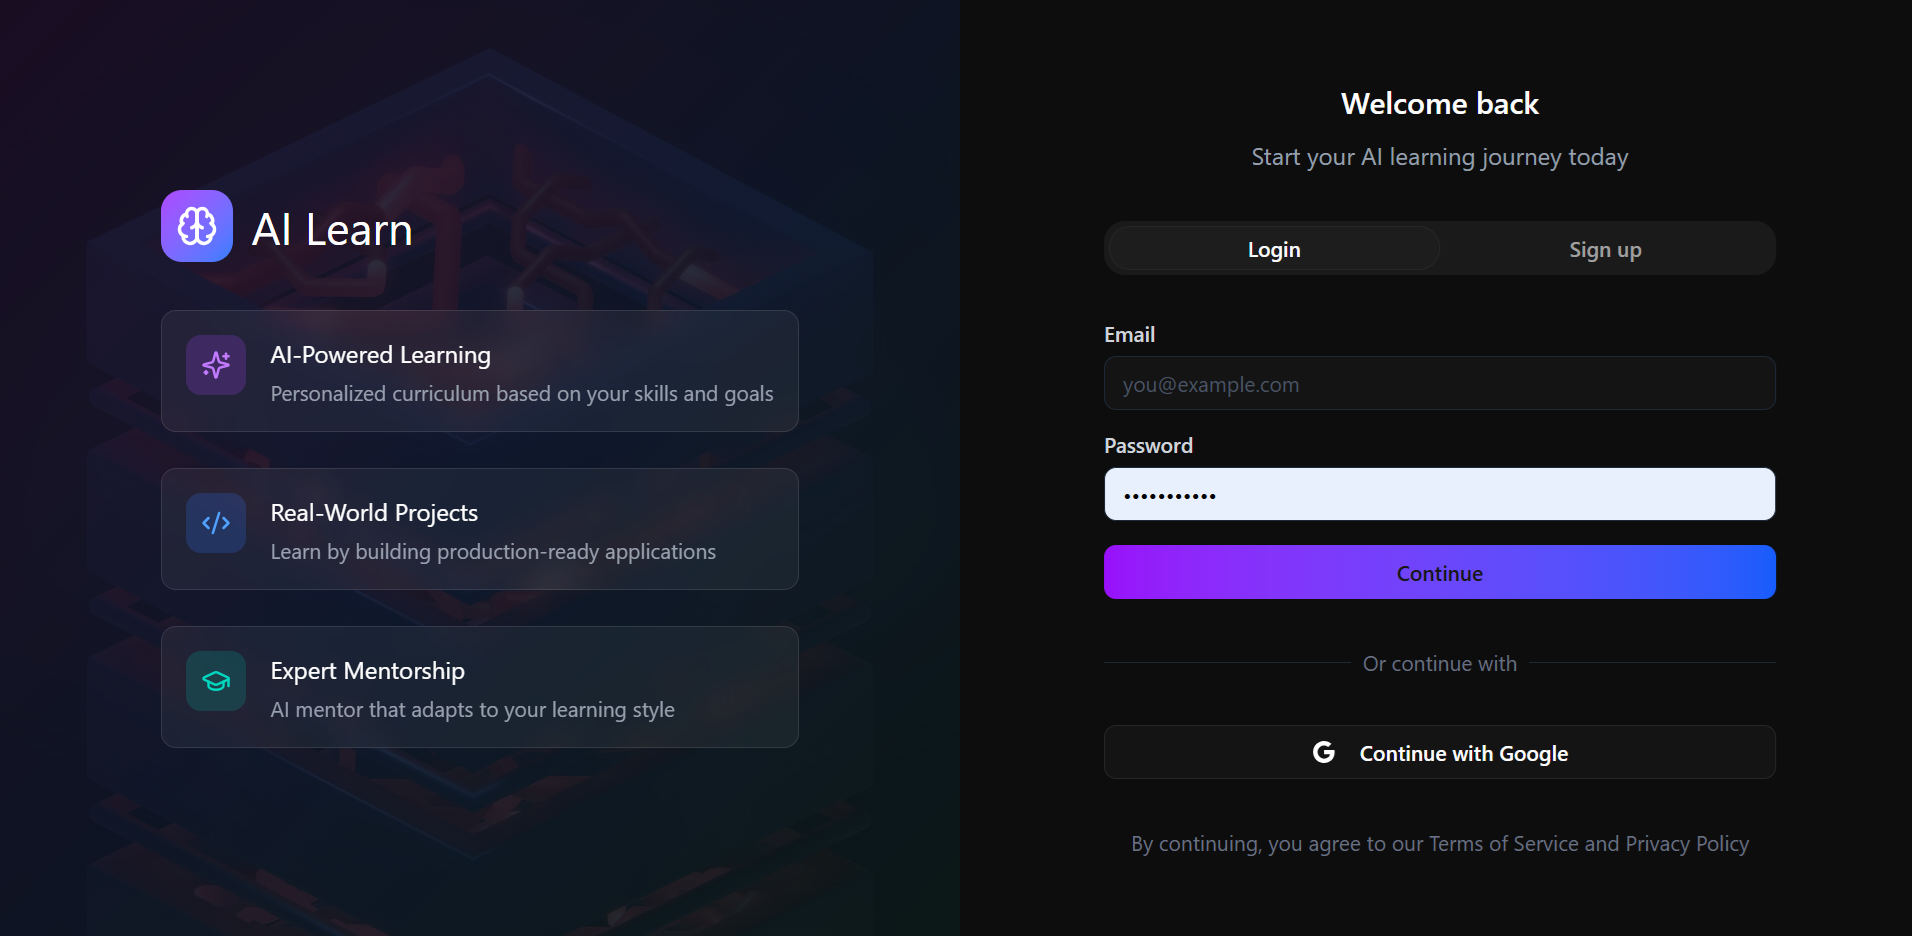
\includegraphics[width=0.9\textwidth]{Figures/login.png}
  \caption{Login screen for users to enter credentials and access the system.}
  \label{fig:login}
\end{figure}

\begin{figure}[H]
    \centering
    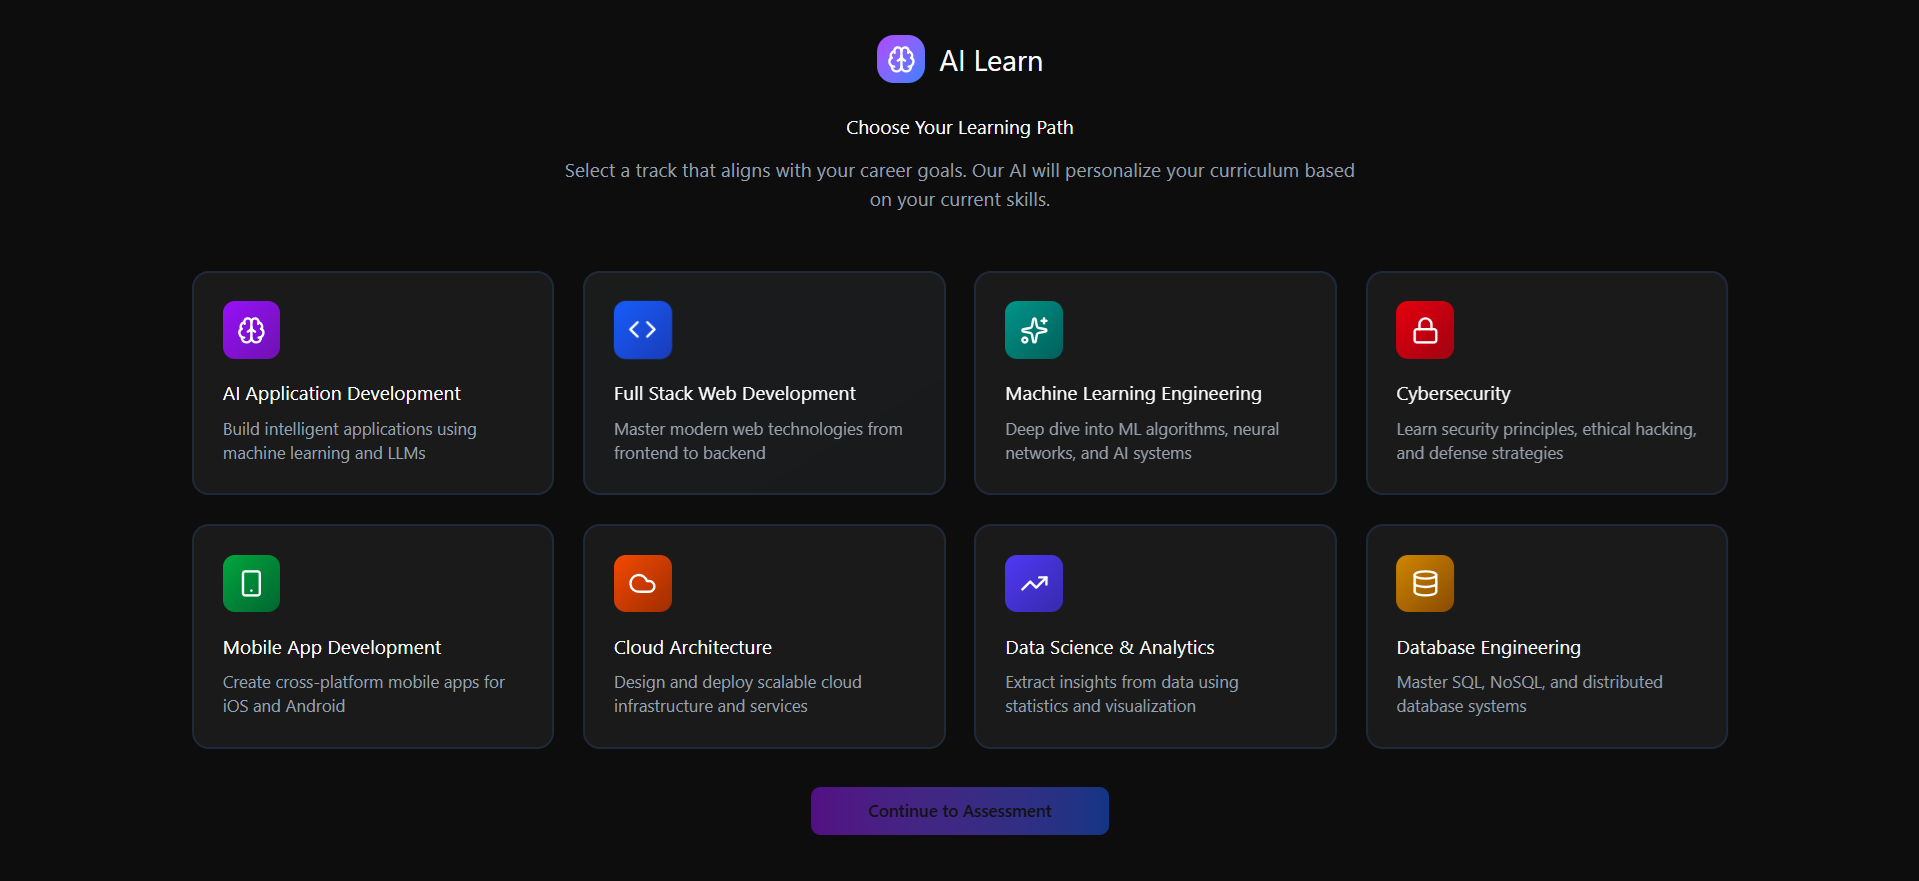
\includegraphics[width=0.9\textwidth]{Figures/Choose Path.png}
    \caption{Track selection screen where users choose their learning path.}
    \label{fig:choose_path}
\end{figure}

\begin{figure}[H]
    \centering
    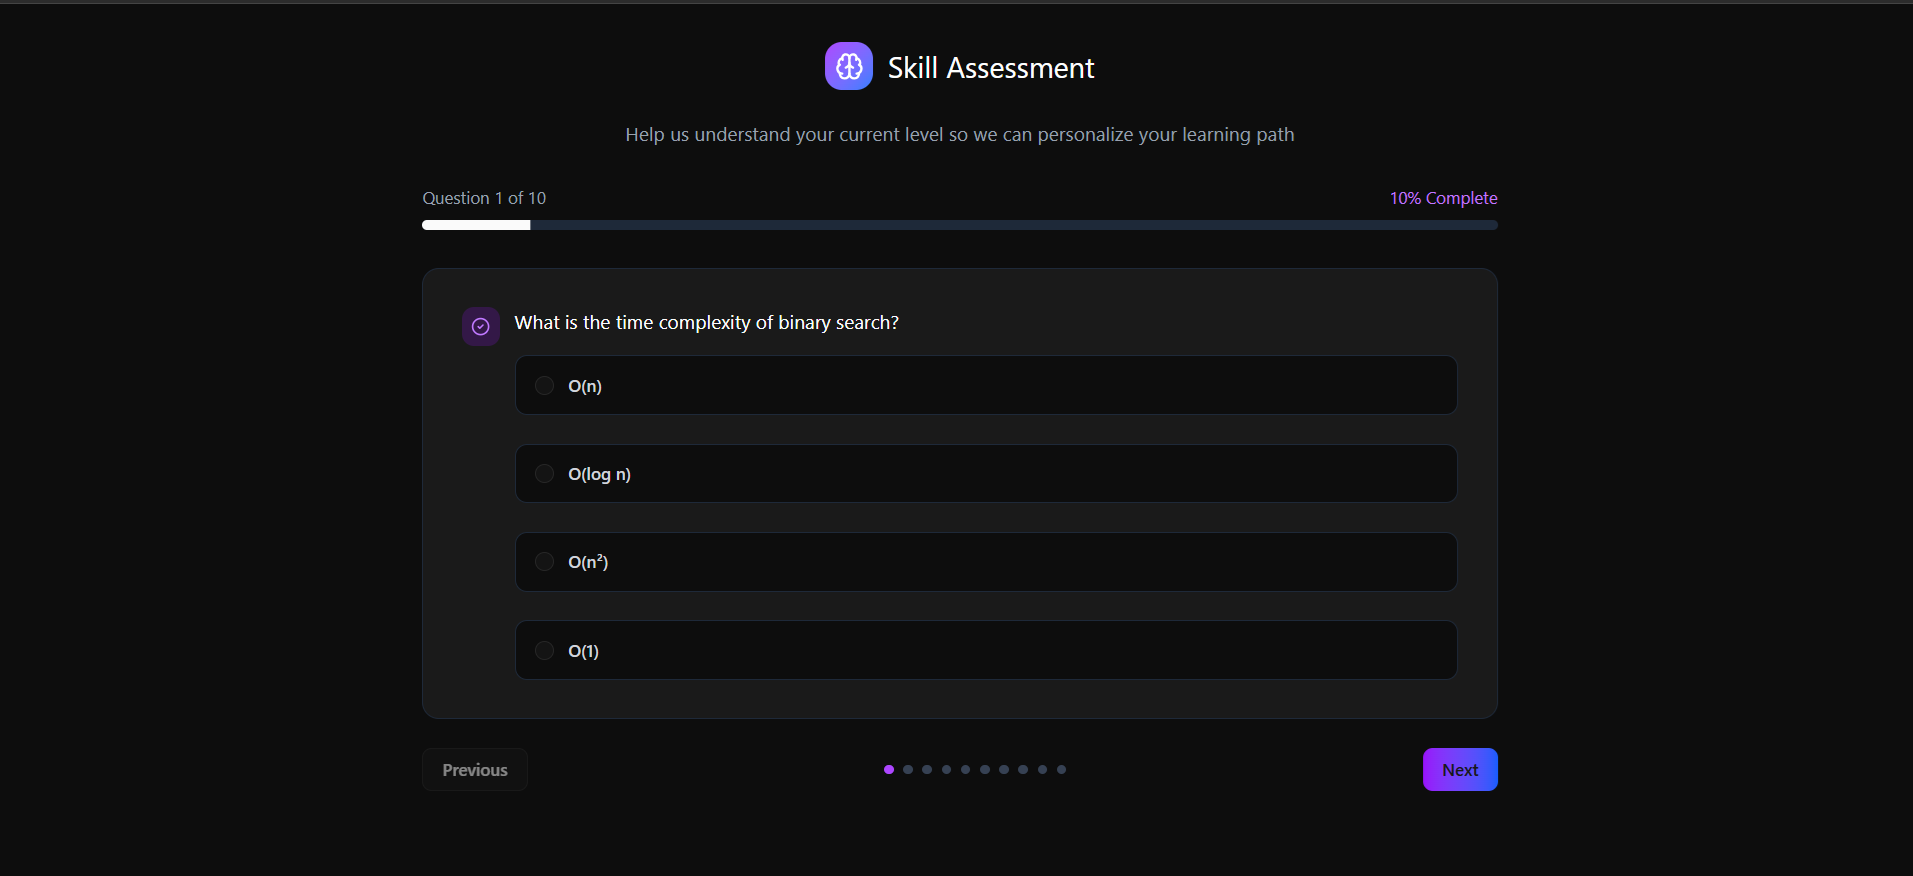
\includegraphics[width=0.9\textwidth]{Figures/skill assesment.png}
    \caption{Skill assessment page for evaluating users’ technical and problem-solving abilities.}
    \label{fig:skill_assessment}
\end{figure}

\begin{figure}[H]
    \centering
    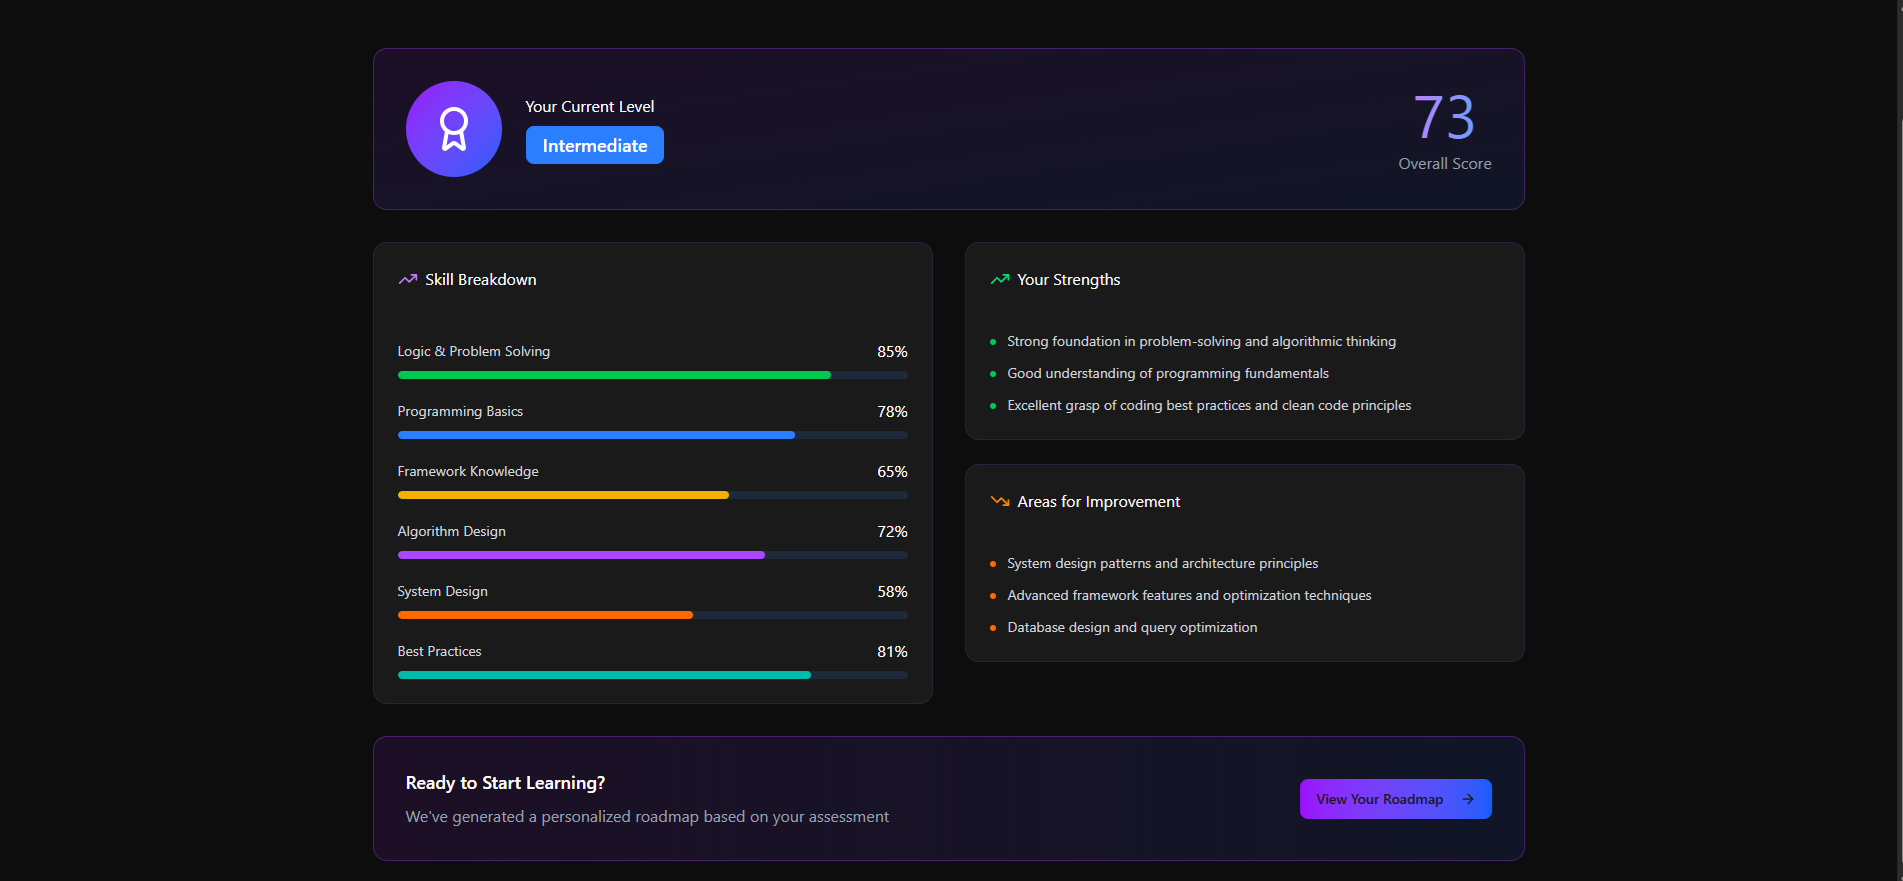
\includegraphics[width=0.9\textwidth]{Figures/Assesment report.png}
    \caption{Assessment report showing the user’s skill level and performance summary.}
    \label{fig:assessment_report}
\end{figure}

\begin{figure}[H]
    \centering
    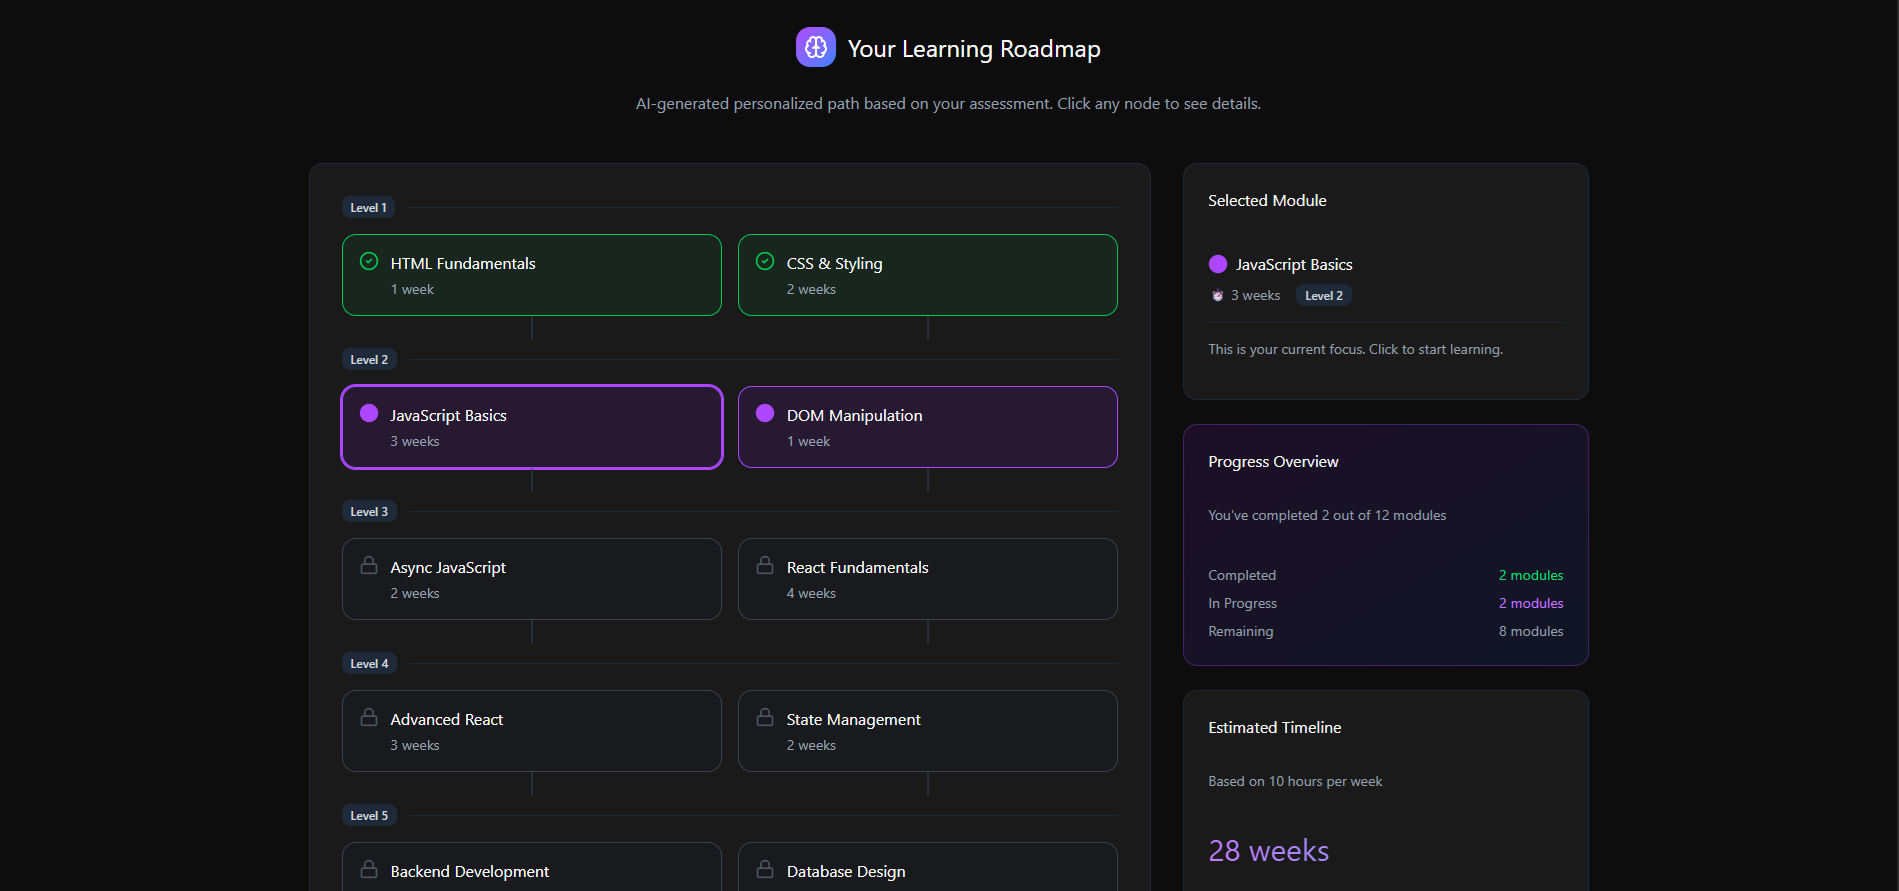
\includegraphics[width=0.9\textwidth]{Figures/roadmap.png}
    \caption{Personalized roadmap showing the AI-generated learning journey and module sequence.}
    \label{fig:roadmap}
\end{figure}

\begin{figure}[H]
    \centering
    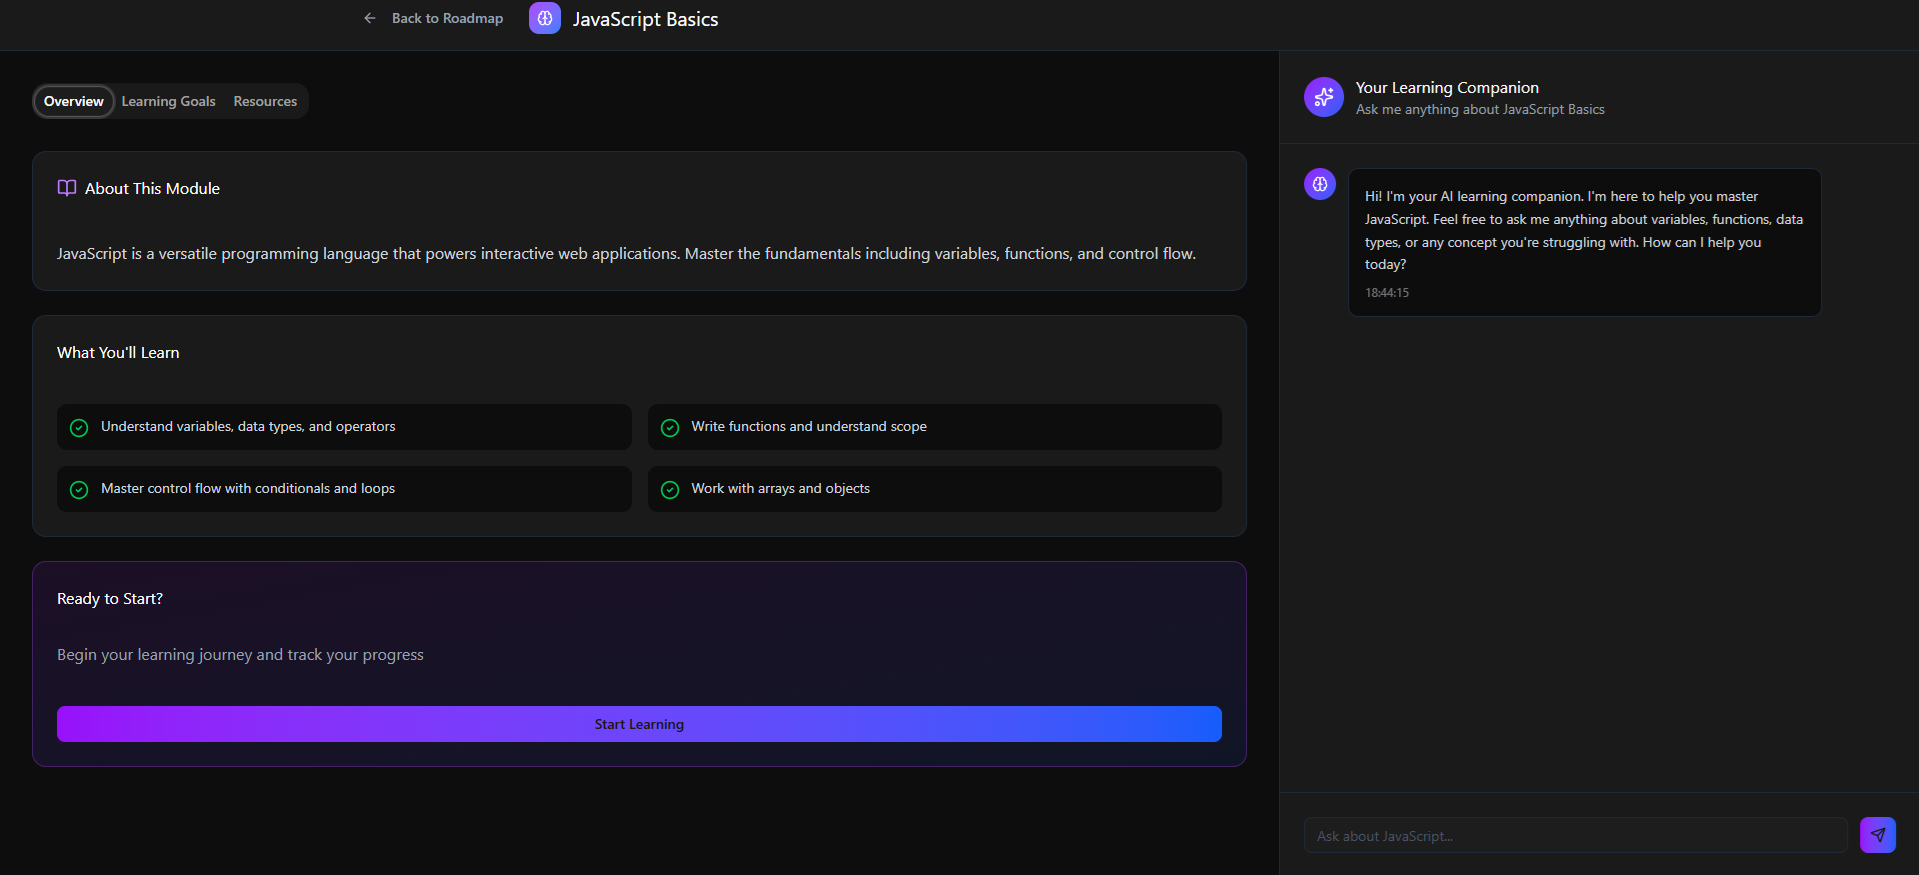
\includegraphics[width=0.9\textwidth]{Figures/module_rag.png}
    \caption{Learning module interface with study content and an integrated AI chatbot.}
    \label{fig:module_rag}
\end{figure}

\begin{figure}[H]
    \centering
    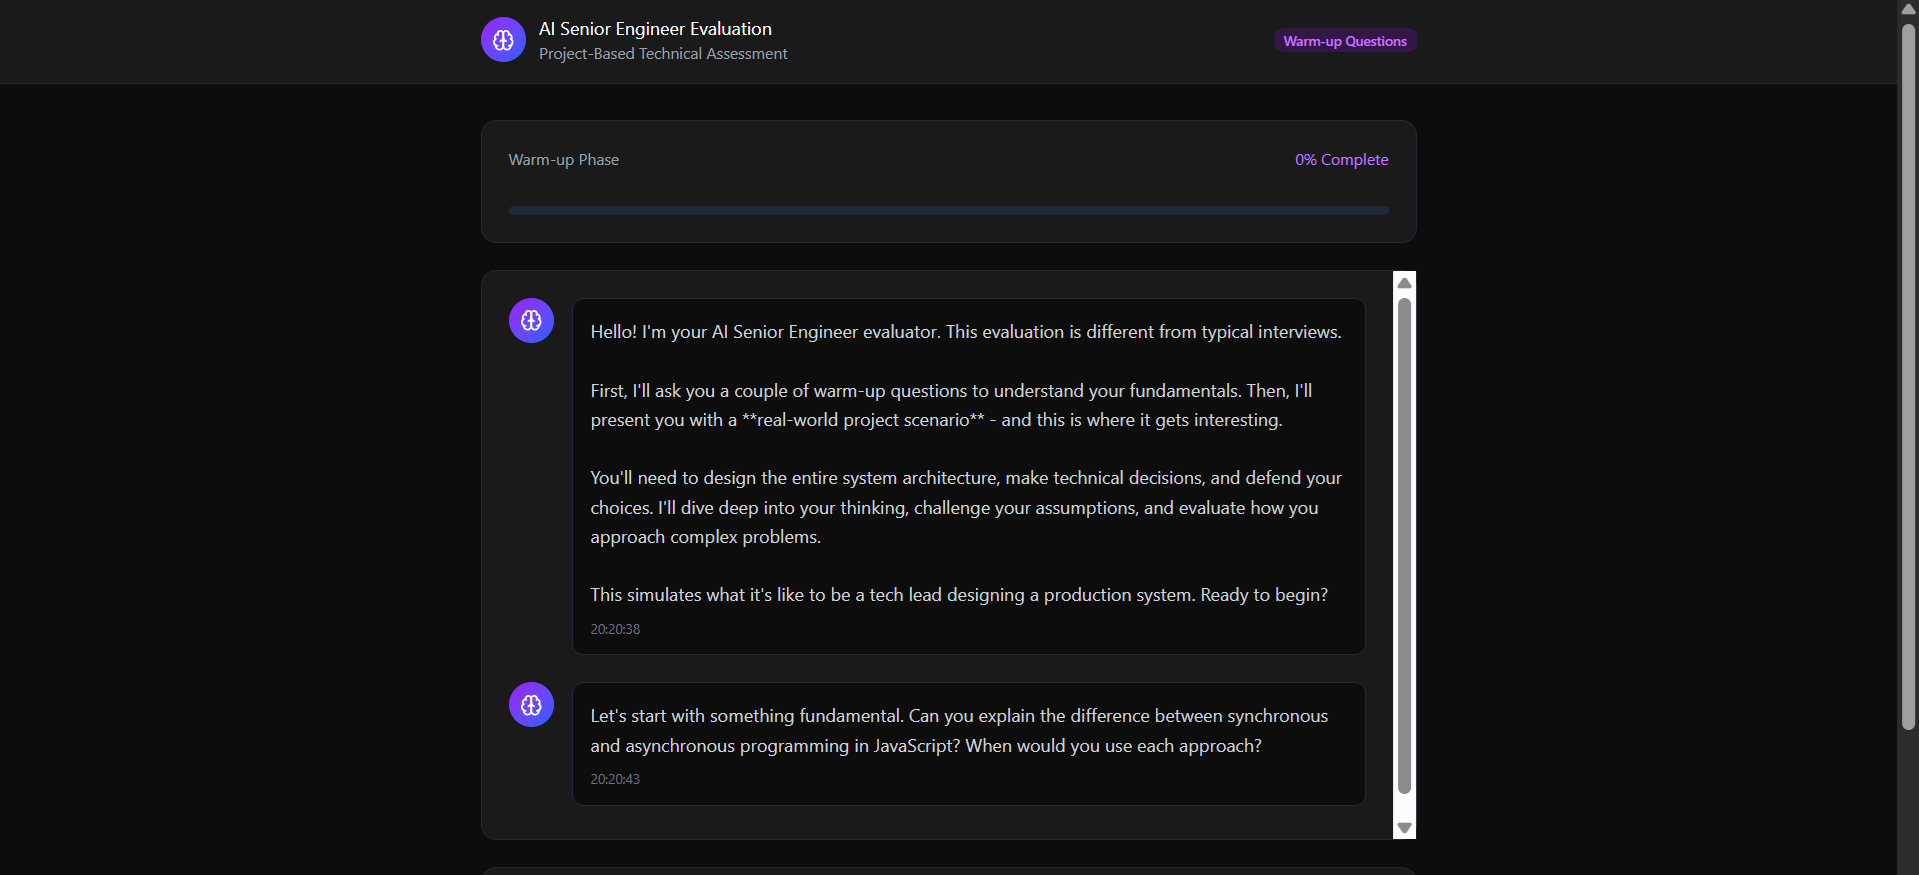
\includegraphics[width=0.9\textwidth]{Figures/Ai Software engineer.png}
    \caption{AI software engineer screen that assigns projects and evaluates user responses.}
    \label{fig:ai_engineer}
\end{figure}

\begin{figure}[H]
    \centering
    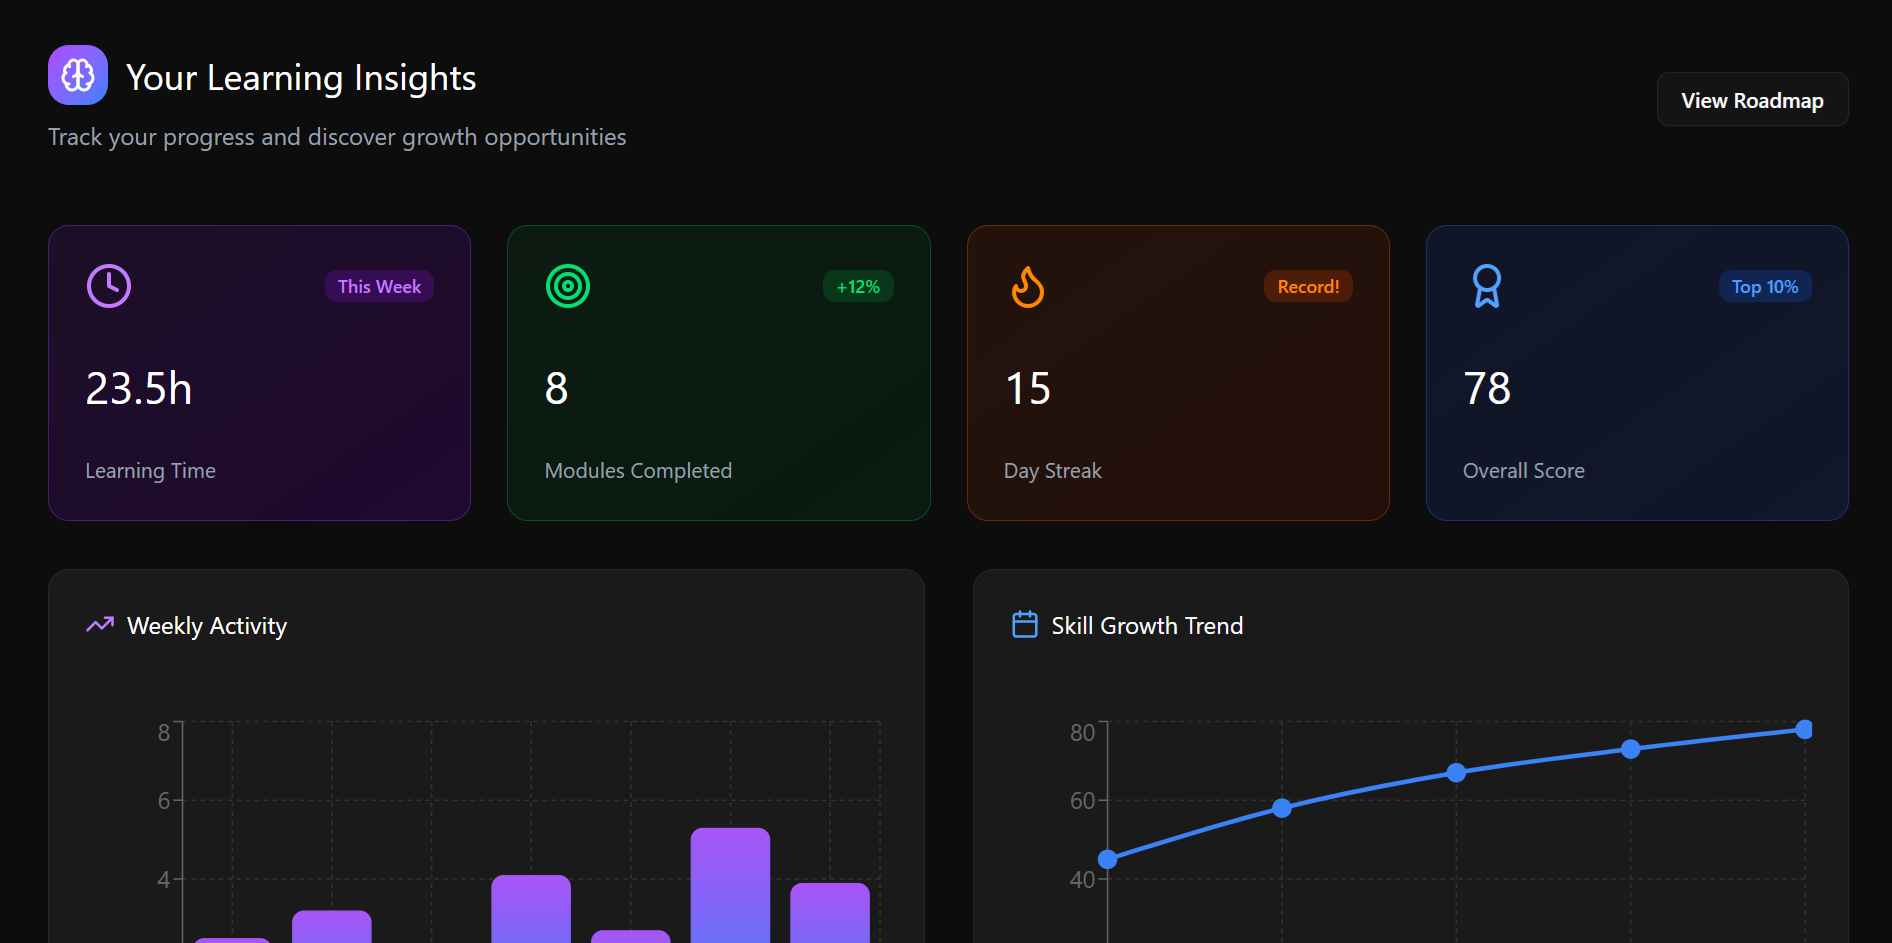
\includegraphics[width=0.9\textwidth]{Figures/Insights.png}
    \caption{Insights dashboard with user progress analytics.}
    \label{fig:insights}
\end{figure}

\begin{figure}[H]
    \centering
    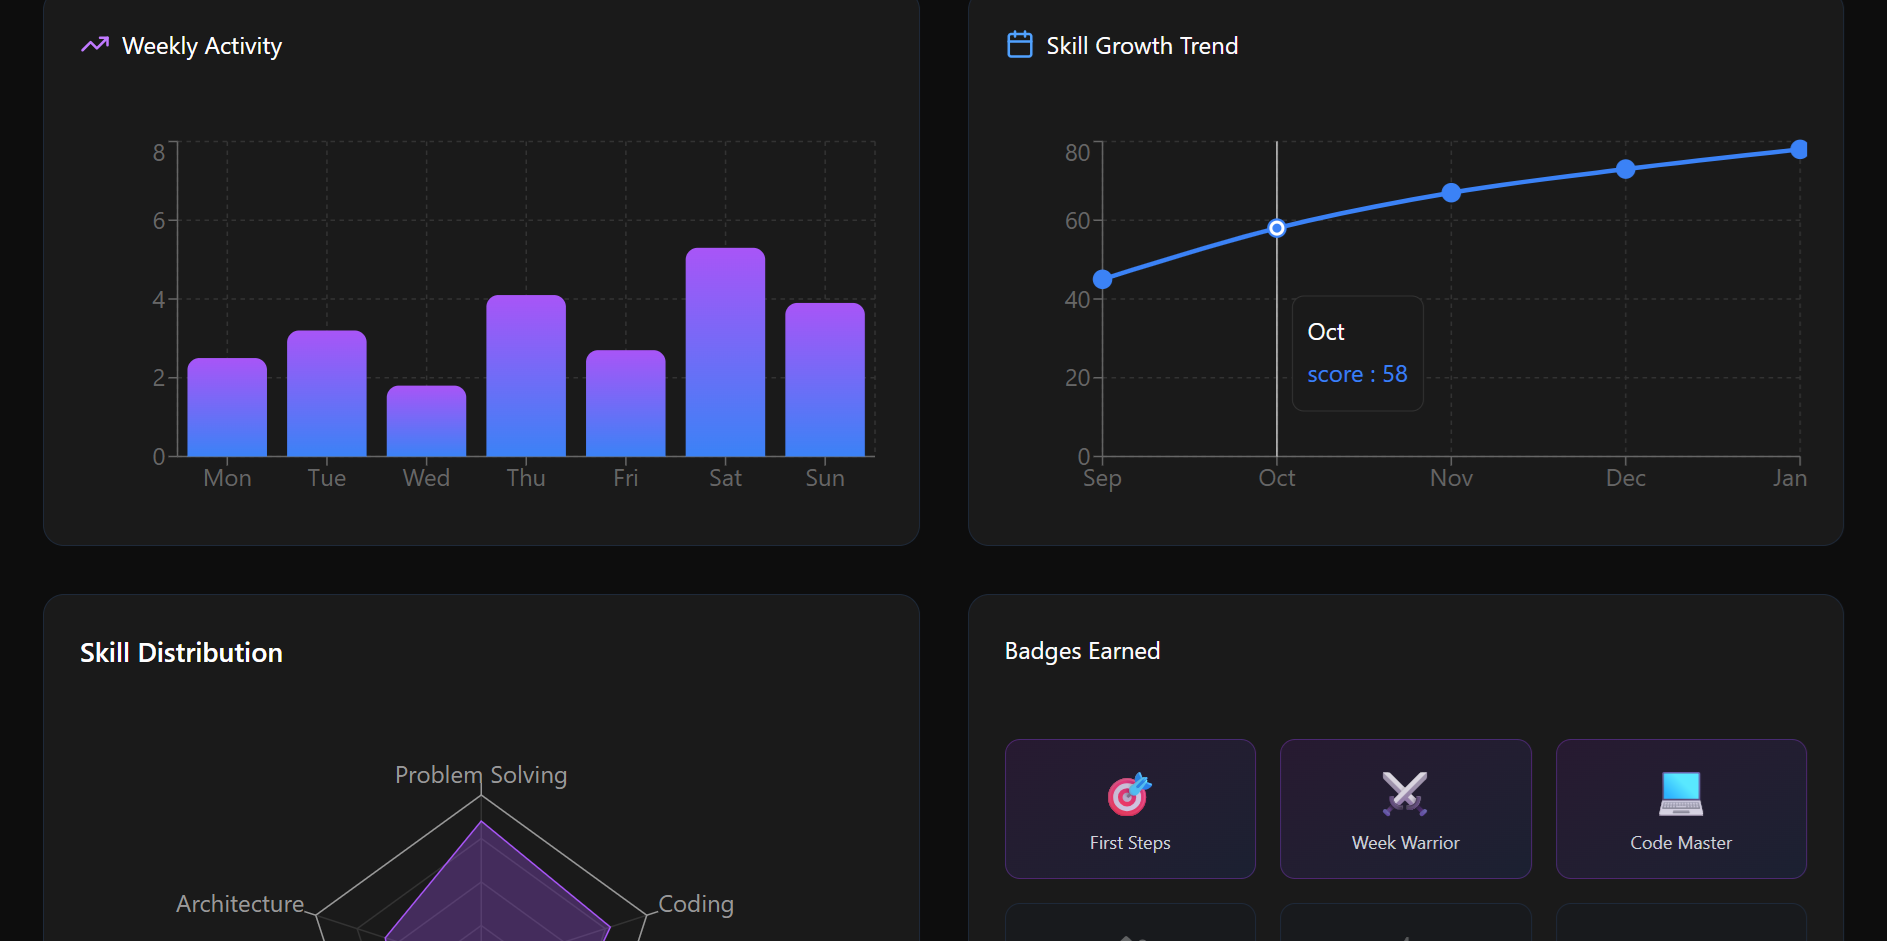
\includegraphics[width=0.9\textwidth]{Figures/Insigth2.png}
    \caption{Advanced insights with AI evaluation and performance graphs.}
    \label{fig:insight2}
\end{figure}

\noindent


\section{Database Design (if required; this means if you are using noSQL, you will not provide ER but the other design element and data dictonary should still be there. Explain and elaborate your DB design)}
\subsection{ER Diagram}

GrowWise runs on PostgreSQL through Supabase as the main relational database. We use the pgvector extension to store and retrieve the embeddings the RAG mentor depends on. The schema follows a normalized relational model organized into four functional modules: user management and authentication, the learning track system, progress and assessment with AI services, and the project workflow and evaluation pipeline.

The entity-relationship diagram below shows the complete schema, including all entities, their attributes, primary and foreign keys, and cardinality constraints. The design keeps data consistent through normalization, supports concurrent users, and can handle the complex queries needed for generating personal learning paths and AI-driven insights.

We structured the schema to support three complementary PlantUML views. View 1 covers the user journey and progress tracking. View 2 focuses on AI services and knowledge management. View 3 covers project workflow and evaluation. The PlantUML files (growwise\_view1\_user\_journey.puml, growwise\_view2\_ai\_services.puml, and growwise\_view3\_projects.puml) give visual representations of the database from each of these perspectives.

\begin{figure}[H]
    \centering
    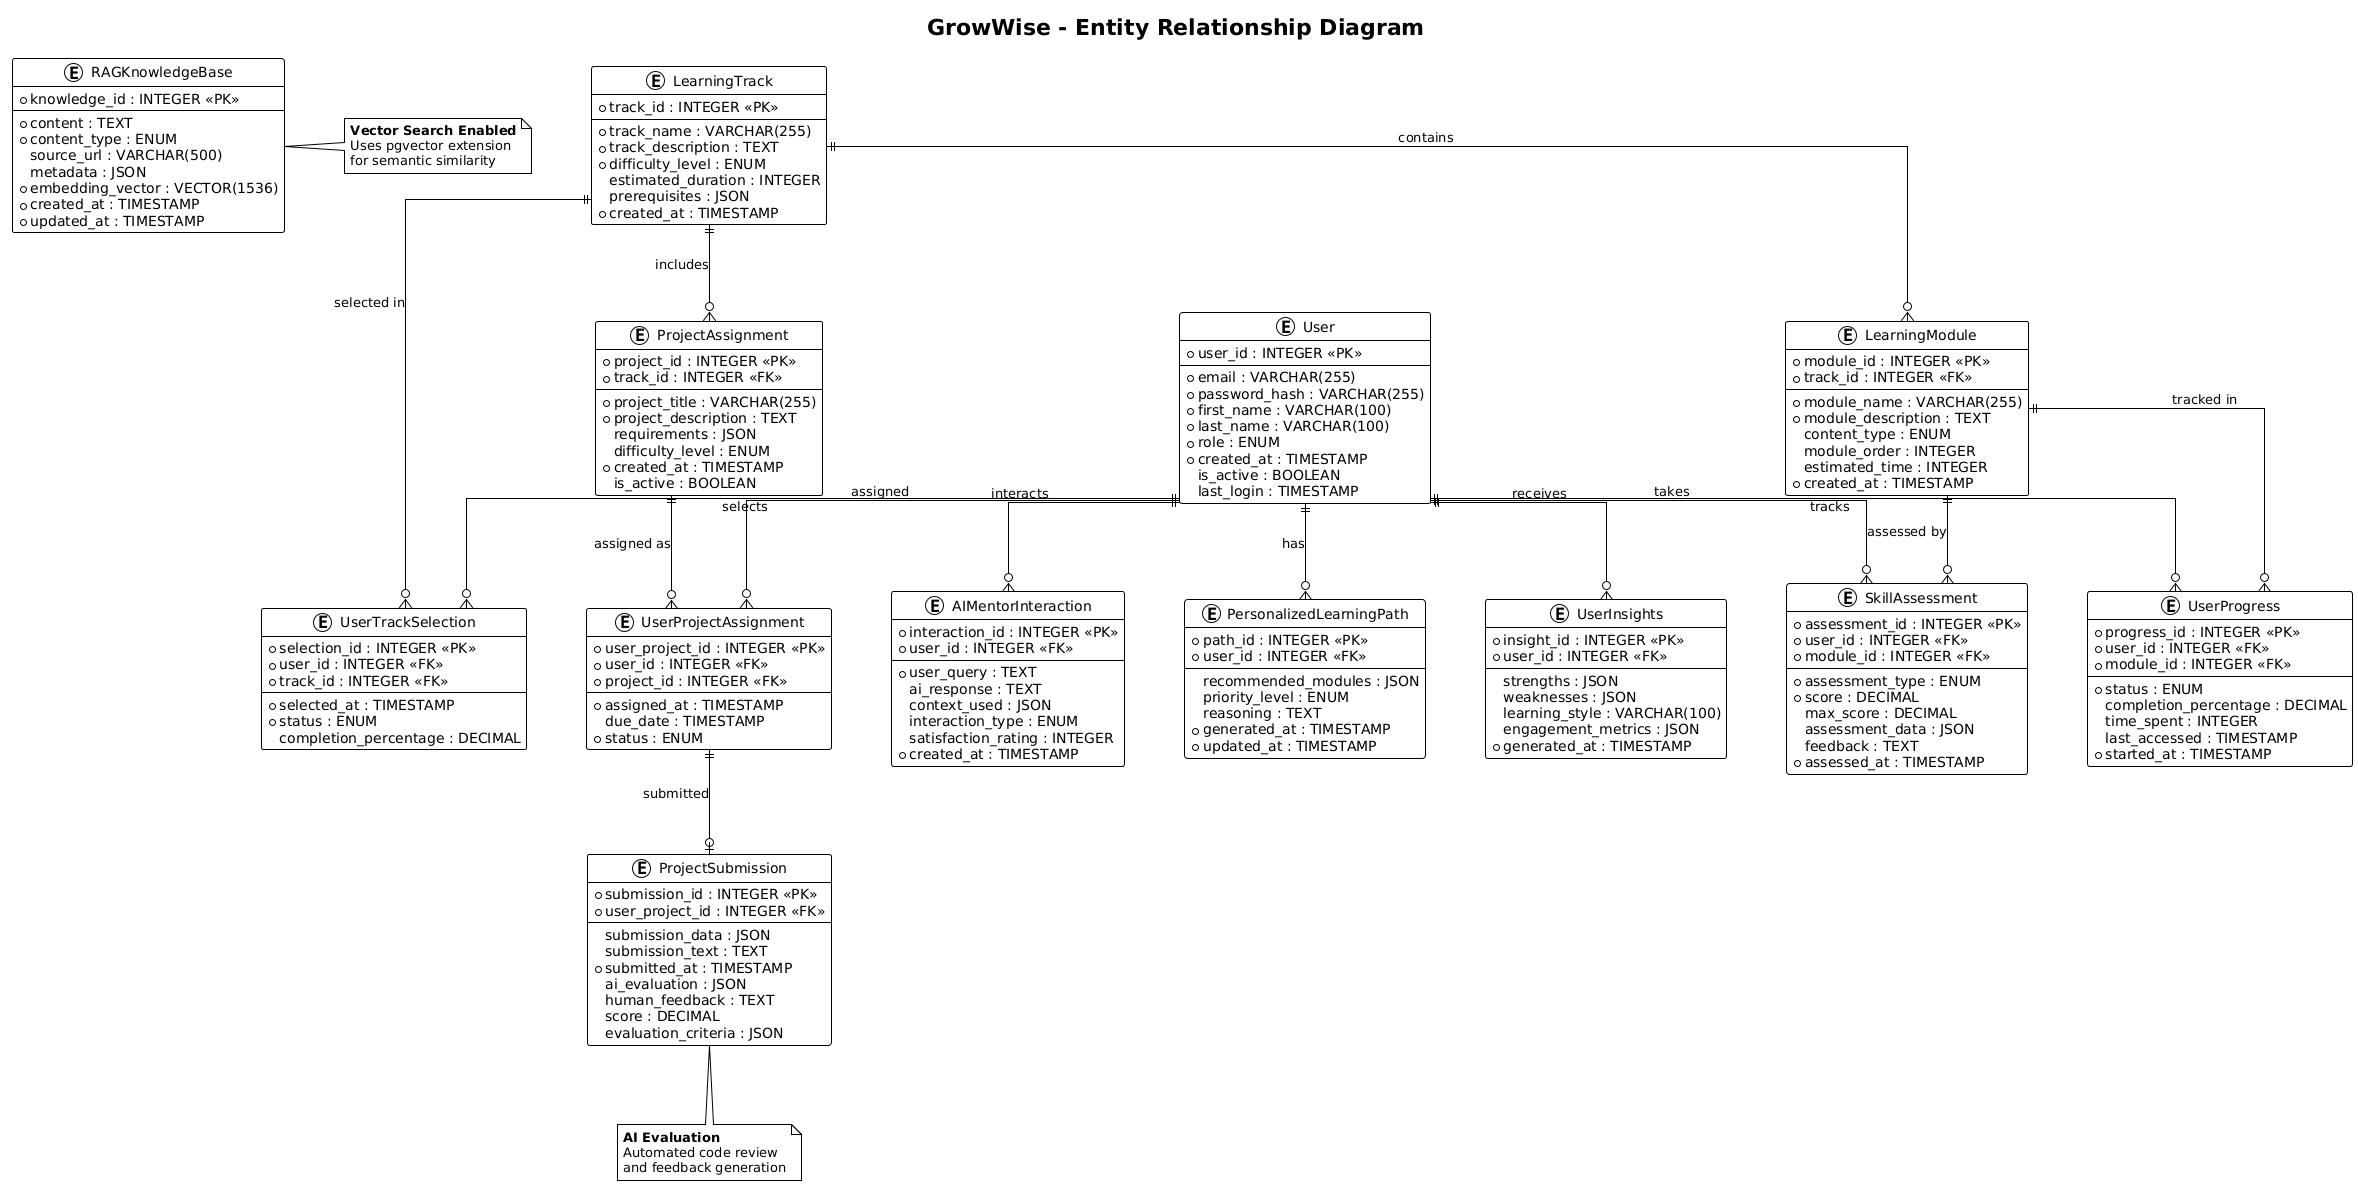
\includegraphics[width=\textwidth]{Figures/ER.png}
    \caption{GrowWise Entity-Relationship Diagram with all entities, keys, and relationships.}
    \label{fig:er_diagram}
\end{figure}

Key database entities and relationships:

\begin{itemize}
    \item User management: The \textit{User} entity is the central anchor. It has one-to-many relationships with UserTrackSelection, UserProgress, SkillAssessment, PersonalizedLearningPath, UserInsights, AIMentorInteraction, and UserProjectAssignment.

    \item Learning content structure: The \textit{LearningTrack} entity has a composition relationship with \textit{LearningModule} (one-to-many). Each track contains multiple ordered modules. Tracks also relate to UserTrackSelection, SkillAssessment, PersonalizedLearningPath, and ProjectAssignment.

    \item Progress tracking: \textit{UserProgress} connects users to specific modules and records completion status and progress percentages. \textit{SkillAssessment} ties users and tracks together to measure proficiency, which then feeds the generation of personalized learning paths.

    \item AI services: \textit{RAGKnowledgeBase} stores module-specific content along with vector embeddings for semantic search. It supports the \textit{AIMentorInteraction} entity, which logs every Q\&A exchange with the AI mentor. \textit{PersonalizedLearningPath} holds the AI-generated module sequences built from assessment results.

    \item Project management: \textit{ProjectAssignment} defines reusable project templates that tie to tracks. \textit{UserProjectAssignment} creates individual project instances for each user. \textit{ProjectSubmission} stores the submitted work along with both AI and human evaluation data.
\end{itemize}

The complete ER diagram, showing every entity, attribute, primary key, foreign key, and cardinality, is rendered through the three PlantUML diagrams referenced above. Together they give a full picture of the GrowWise database.

\subsection{Data Dictionary}

The data dictionary documents every table, its columns, data types, constraints, and purpose. This section captures the full schema for the GrowWise platform, grouped by functional module for easier navigation and maintenance. Each entry lists the column name, its data type, applicable constraints such as primary keys, foreign keys, uniqueness, and null rules, along with a short description of what the column represents.



\begin{samepage}


\begin{table}[H]
\footnotesize
\centering
\caption{Test case for User}
\begin{tabular}{|p{3cm}|p{2.3cm}|p{3.8cm}|p{4.4cm}|}
\hline
Attribute Name & Data Type & Constraints & Description \\ \hline
user\_id & INTEGER & PK, AUTO\newline INCREMENT,\newline NOT NULL & Unique identifier for each user \\ \hline
email & VARCHAR(255) & UNIQUE,\newline NOT NULL & User's email address for login and communication \\ \hline
password\_hash & VARCHAR(255) & NOT NULL & Hashed password for secure authentication \\ \hline
first\_name & VARCHAR(100) & NOT NULL & User's first name \\ \hline
last\_name & VARCHAR(100) & NOT NULL & User's last name \\ \hline
user\_type & ENUM('learner', 'admin') & NOT NULL,\newline DEFAULT 'learner' & Role-based user classification \\ \hline
created\_at & TIMESTAMP & NOT NULL,\newline DEFAULT\newline CURRENT\_TIMESTAMP & Account creation timestamp \\ \hline
is\_active & BOOLEAN & NOT NULL,\newline DEFAULT TRUE & Account status flag \\ \hline
\end{tabular}
\end{table}
\end{samepage}



\begin{samepage}


\begin{table}[H]
\footnotesize
\centering
\caption{Test case for LearningTrack}
\begin{tabular}{|p{3cm}|p{2.3cm}|p{3.8cm}|p{4.4cm}|}
\hline
Attribute Name & Data Type & Constraints & Description \\ \hline
track\_id & INTEGER & PK, AUTO\newline INCREMENT,\newline NOT NULL & Unique identifier for each learning track \\ \hline
track\_name & VARCHAR(200) & NOT NULL & Name of the learning track (e.g., "Web Development", "AI/ML") \\ \hline
description & TEXT & NULL & Detailed description of track goals and curriculum \\ \hline
difficulty\_level & ENUM('beginner', 'intermediate', 'advanced') & NOT NULL & Overall difficulty rating of the track \\ \hline
estimated\_duration\_hours & INTEGER & NOT NULL & Approximate time required to complete the track \\ \hline
\end{tabular}
\end{table}
\end{samepage}

\begin{samepage}


\begin{table}[H]
\footnotesize
\centering
\caption{Test case for LearningModule}
\begin{tabular}{|p{3cm}|p{2.3cm}|p{3.8cm}|p{4.4cm}|}
\hline
Attribute Name & Data Type & Constraints & Description \\ \hline
module\_id & INTEGER & PK, AUTO\newline INCREMENT,\newline NOT NULL & Unique identifier for each module \\ \hline
track\_id & INTEGER & FK(LearningTrack),\newline NOT NULL & Reference to parent learning track \\ \hline
module\_name & VARCHAR(200) & NOT NULL & Name of the learning module \\ \hline
module\_order & INTEGER & NOT NULL & Sequence position within the track \\ \hline
content\_type & ENUM('video', 'text', 'interactive', 'quiz') & NOT NULL & Type of learning content \\ \hline
estimated\_duration\_minutes & INTEGER & NOT NULL & Expected completion time for this module \\ \hline
learning\_objectives & TEXT & NULL & Specific learning goals for this module \\ \hline
\end{tabular}
\end{table}
\end{samepage}

\begin{samepage}


\begin{table}[H]
\footnotesize
\centering
\caption{Test case for UserTrackSelection}
\begin{tabular}{|p{3cm}|p{2.3cm}|p{3.8cm}|p{4.4cm}|}
\hline
Attribute Name & Data Type & Constraints & Description \\ \hline
selection\_id & INTEGER & PK, AUTO\newline INCREMENT,\newline NOT NULL & Unique identifier for each selection \\ \hline
user\_id & INTEGER & FK(User),\newline NOT NULL & Reference to the user making the selection \\ \hline
track\_id & INTEGER & FK(LearningTrack),\newline NOT NULL & Reference to the selected track \\ \hline
selected\_at & TIMESTAMP & NOT NULL,\newline DEFAULT\newline CURRENT\_TIMESTAMP & When the track was selected \\ \hline
is\_active & BOOLEAN & NOT NULL,\newline DEFAULT TRUE & Whether this selection is currently active \\ \hline
\end{tabular}
\end{table}
\end{samepage}



\begin{samepage}


\begin{table}[H]
\footnotesize
\centering
\caption{Test case for UserProgress}
\begin{tabular}{|p{3cm}|p{2.3cm}|p{3.8cm}|p{4.4cm}|}
\hline
Attribute Name & Data Type & Constraints & Description \\ \hline
progress\_id & INTEGER & PK, AUTO\newline INCREMENT,\newline NOT NULL & Unique identifier for each progress record \\ \hline
user\_id & INTEGER & FK(User),\newline NOT NULL & Reference to the user \\ \hline
module\_id & INTEGER & FK(LearningModule),\newline NOT NULL & Reference to the learning module \\ \hline
status & ENUM('not\_started', 'in\_progress', 'completed') & NOT NULL,\newline DEFAULT\newline 'not\_started' & Current completion status \\ \hline
started\_at & TIMESTAMP & NULL & When the user began this module \\ \hline
completed\_at & TIMESTAMP & NULL & When the user completed this module \\ \hline
progress\_percentage & DECIMAL(5,2) & NOT NULL,\newline DEFAULT 0.00 & Percentage of module completed (0-100) \\ \hline
\end{tabular}
\end{table}
\end{samepage}

\begin{samepage}


\begin{table}[H]
\footnotesize
\centering
\caption{Test case for SkillAssessment}
\begin{tabular}{|p{3cm}|p{2.3cm}|p{3.8cm}|p{4.4cm}|}
\hline
Attribute Name & Data Type & Constraints & Description \\ \hline
assessment\_id & INTEGER & PK, AUTO\newline INCREMENT,\newline NOT NULL & Unique identifier for each assessment \\ \hline
user\_id & INTEGER & FK(User),\newline NOT NULL & Reference to the assessed user \\ \hline
track\_id & INTEGER & FK(LearningTrack),\newline NOT NULL & Track being assessed \\ \hline
total\_questions & INTEGER & NOT NULL & Total number of assessment questions \\ \hline
score\_percentage & DECIMAL(5,2) & NOT NULL & User's score (0-100) \\ \hline
assessment\_data & JSON & NULL & Detailed question-by-question results \\ \hline
completed\_at & TIMESTAMP & NOT NULL,\newline DEFAULT\newline CURRENT\_TIMESTAMP & Assessment completion time \\ \hline
\end{tabular}
\end{table}
\end{samepage}

\begin{samepage}


\begin{table}[H]
\footnotesize
\centering
\caption{Test case for PersonalizedLearningPath}
\begin{tabular}{|p{3cm}|p{2.3cm}|p{3.8cm}|p{4.4cm}|}
\hline
Attribute Name & Data Type & Constraints & Description \\ \hline
path\_id & INTEGER & PK, AUTO\newline INCREMENT,\newline NOT NULL & Unique identifier for each learning path \\ \hline
user\_id & INTEGER & FK(User),\newline NOT NULL & Reference to the user \\ \hline
track\_id & INTEGER & FK(LearningTrack),\newline NOT NULL & Reference to the learning track \\ \hline
assessment\_id & INTEGER & FK(SkillAssessment),\newline NULL & Assessment that generated this path \\ \hline
path\_data & JSON & NOT NULL & AI-generated sequence of modules and milestones \\ \hline
status & ENUM('active', 'completed', 'archived') & NOT NULL,\newline DEFAULT 'active' & Current path status \\ \hline
created\_at & TIMESTAMP & NOT NULL,\newline DEFAULT\newline CURRENT\_TIMESTAMP & Path generation timestamp \\ \hline
\end{tabular}
\end{table}
\end{samepage}

\begin{samepage}


\begin{table}[H]
\footnotesize
\centering
\caption{Test case for UserInsights}
\begin{tabular}{|p{3cm}|p{2.3cm}|p{3.8cm}|p{4.4cm}|}
\hline
Attribute Name & Data Type & Constraints & Description \\ \hline
insight\_id & INTEGER & PK, AUTO\newline INCREMENT,\newline NOT NULL & Unique identifier for each insight \\ \hline
user\_id & INTEGER & FK(User),\newline NOT NULL & Reference to the user \\ \hline
insight\_type & ENUM('strength', 'weakness', 'recommendation', 'milestone') & NOT NULL & Category of insight \\ \hline
insight\_data & JSON & NOT NULL & Detailed insight content and metrics \\ \hline
priority & ENUM('low', 'medium', 'high') & NOT NULL,\newline DEFAULT 'medium' & Importance level of the insight \\ \hline
created\_at & TIMESTAMP & NOT NULL,\newline DEFAULT\newline CURRENT\_TIMESTAMP & Insight generation timestamp \\ \hline
\end{tabular}
\end{table}
\end{samepage}



\begin{samepage}


\begin{table}[H]
\footnotesize
\centering
\caption{Test case for RAGKnowledgeBase}
\begin{tabular}{|p{3cm}|p{2.3cm}|p{3.8cm}|p{4.4cm}|}
\hline
Attribute Name & Data Type & Constraints & Description \\ \hline
knowledge\_id & INTEGER & PK, AUTO\newline INCREMENT,\newline NOT NULL & Unique identifier for each knowledge entry \\ \hline
module\_id & INTEGER & FK(LearningModule),\newline NULL & Associated learning module \\ \hline
content\_type & ENUM('documentation', 'example', 'explanation', 'reference') & NOT NULL & Type of knowledge content \\ \hline
title & VARCHAR(300) & NOT NULL & Title or heading of the knowledge entry \\ \hline
content & TEXT & NOT NULL & Full text content for retrieval \\ \hline
metadata & JSON & NULL & Additional structured information \\ \hline
embedding\_vector & VECTOR(1536) & NOT NULL & Vector embedding for semantic search (pgvector) \\ \hline
is\_active & BOOLEAN & NOT NULL,\newline DEFAULT TRUE & Whether this entry is currently searchable \\ \hline
created\_at & TIMESTAMP & NOT NULL,\newline DEFAULT\newline CURRENT\_TIMESTAMP & Entry creation timestamp \\ \hline
\end{tabular}
\end{table}
\end{samepage}

\begin{samepage}


\begin{table}[H]
\footnotesize
\centering
\caption{Test case for AIMentorInteraction}
\begin{tabular}{|p{3cm}|p{2.3cm}|p{3.8cm}|p{4.4cm}|}
\hline
Attribute Name & Data Type & Constraints & Description \\ \hline
interaction\_id & INTEGER & PK, AUTO\newline INCREMENT,\newline NOT NULL & Unique identifier for each interaction \\ \hline
user\_id & INTEGER & FK(User),\newline NOT NULL & Reference to the user asking the question \\ \hline
module\_id & INTEGER & FK(LearningModule),\newline NULL & Context module if applicable \\ \hline
user\_question & TEXT & NOT NULL & User's original question \\ \hline
ai\_response & TEXT & NOT NULL & AI-generated response \\ \hline
context\_data & JSON & NULL & Retrieved RAG context and sources \\ \hline
response\_time\_ms & INTEGER & NULL & Response generation time in milliseconds \\ \hline
feedback\_rating & INTEGER & NULL, CHECK\newline (feedback\_rating\newline BETWEEN 1\newline AND 5) & User satisfaction rating (1-5) \\ \hline
created\_at & TIMESTAMP & NOT NULL,\newline DEFAULT\newline CURRENT\_TIMESTAMP & Interaction timestamp \\ \hline
\end{tabular}
\end{table}
\end{samepage}



\begin{samepage}


\begin{table}[H]
\footnotesize
\centering
\caption{Test case for ProjectAssignment}
\begin{tabular}{|p{3cm}|p{2.3cm}|p{3.8cm}|p{4.4cm}|}
\hline
Attribute Name & Data Type & Constraints & Description \\ \hline
project\_id & INTEGER & PK, AUTO\newline INCREMENT,\newline NOT NULL & Unique identifier for each project template \\ \hline
track\_id & INTEGER & FK(LearningTrack),\newline NOT NULL & Associated learning track \\ \hline
project\_title & VARCHAR(300) & NOT NULL & Name of the project \\ \hline
project\_description & TEXT & NOT NULL & Detailed project requirements and objectives \\ \hline
requirements & JSON & NOT NULL & Technical and functional requirements \\ \hline
difficulty\_level & ENUM('beginner', 'intermediate', 'advanced') & NOT NULL & Project complexity level \\ \hline
created\_at & TIMESTAMP & NOT NULL,\newline DEFAULT\newline CURRENT\_TIMESTAMP & Project creation timestamp \\ \hline
is\_active & BOOLEAN & NOT NULL,\newline DEFAULT TRUE & Whether project is currently assignable \\ \hline
\end{tabular}
\end{table}
\end{samepage}

\begin{samepage}


\begin{table}[H]
\footnotesize
\centering
\caption{Test case for UserProjectAssignment}
\begin{tabular}{|p{3cm}|p{2.3cm}|p{3.8cm}|p{4.4cm}|}
\hline
Attribute Name & Data Type & Constraints & Description \\ \hline
user\_project\_id & INTEGER & PK, AUTO\newline INCREMENT,\newline NOT NULL & Unique identifier for each user assignment \\ \hline
user\_id & INTEGER & FK(User),\newline NOT NULL & Reference to the assigned user \\ \hline
project\_id & INTEGER & FK(ProjectAssignment),\newline NOT NULL & Reference to the project template \\ \hline
assigned\_at & TIMESTAMP & NOT NULL,\newline DEFAULT\newline CURRENT\_TIMESTAMP & Assignment timestamp \\ \hline
due\_date & TIMESTAMP & NULL & Project deadline \\ \hline
status & ENUM('assigned', 'in\_progress', 'submitted', 'evaluated') & NOT NULL,\newline DEFAULT\newline 'assigned' & Current project status \\ \hline
\end{tabular}
\end{table}
\end{samepage}

\begin{samepage}


\begin{table}[H]
\footnotesize
\centering
\caption{Test case for ProjectSubmission}
\begin{tabular}{|p{3cm}|p{2.3cm}|p{3.8cm}|p{4.4cm}|}
\hline
Attribute Name & Data Type & Constraints & Description \\ \hline
submission\_id & INTEGER & PK, AUTO\newline INCREMENT,\newline NOT NULL & Unique identifier for each submission \\ \hline
user\_project\_id & INTEGER & FK(UserProjectAssignment),\newline NOT NULL & Reference to the user's project assignment \\ \hline
submission\_data & JSON & NOT NULL & Project files, links, and deliverables \\ \hline
submission\_text & TEXT & NULL & User's written explanation or documentation \\ \hline
submitted\_at & TIMESTAMP & NOT NULL,\newline DEFAULT\newline CURRENT\_TIMESTAMP & Submission timestamp \\ \hline
ai\_evaluation & JSON & NULL & AI-generated evaluation results and feedback \\ \hline
human\_feedback & TEXT & NULL & Optional instructor or admin feedback \\ \hline
score & DECIMAL(5,2) & NULL & Final project score (0-100) \\ \hline
evaluation\_criteria & JSON & NULL & Rubric and evaluation breakdown \\ \hline
\end{tabular}
\end{table}
\end{samepage}

\section{Risk Analysis}

This section covers potential project risks and how we plan to address them.

\subsection{Technical Risks}

The platform can run into bugs, server outages, or incorrect AI responses. The OpenAI and Gemini APIs can also change without much warning or go down entirely. We mitigate this through thorough testing and a fallback plan that can switch providers if needed.

\subsection{Business Risks}

The online learning space is crowded, so gaining users is difficult. API and infrastructure costs can climb quickly. We believe the platform's personalization and project-based evaluation set it apart, and we monitor costs closely to keep the model sustainable.

A second risk is content quality. The AI can produce incorrect or outdated information, and sometimes adds unnecessary details. We plan to review and refine the content regularly to keep it accurate.

\subsection{User Risks}

Some users might find the platform difficult or lose motivation along the way. We address this with a clean, approachable design and an AI mentor that guides learners step by step.

\subsection{Security Risks}

Users log in and share personal information. Weak security can lead to data loss or exposure. We mitigate this through secure hosting, strong password policies, and protective measures across all user data.

\section*{Conclusion}

This chapter covered the core specifications for GrowWise. It described what the system does, how users and admins interact with it, and how the components fit together. The functional and non-functional requirements are carefully defined so the platform stays fast, reliable, and easy to use. We discussed quality attributes such as performance, usability, and scalability, which all feed into the user experience. The chapter also covered assumptions, hardware and software needs, and likely development risks. On top of that, the use cases, UI designs, and database structure show how modules fit together and how the system operates end to end. Together, these specifications give us a clear plan for building, testing, and improving the platform.

\chapter{High-Level and Low-Level Design}

This chapter tell high level and low level design of our project.

\section{System Overview}

GrowWise is smart AI learning app that make study personal for developer. It check learner skill now, make special path for them, and give smart help with Agentic RAG teacher inside. The system care about teach how to think and do real project to make good problem solving skill.

\subsection{Learning Management and Modules}

GrowWise put content in small interactive lesson call learning node. Got clear goal, example and real task to do. User go step by step on AI make roadmap. Got check if you ready before next and auto track how you do.

\subsection{Personalized Learning Paths}

AI planner look your first test and what track you pick. Then make special roadmap only for you. When you study it change path auto from how fast you learn, what you good at and what need more time. So you not study same thing again or jump to too hard too quick.

\subsection{Agentic RAG Mentor (Context-Aware Assistance)}

You got smart AI teacher inside app. It find best resource for your lesson now and give easy explain right when you need. You ask anything it answer question, give clear tip and show helpful thing that match what you do now and what you did before.

\subsection{Assessment and AI Software Engineer Evaluation}

You do quiz, small task and real project challenge. One fake AI engineer check your work same like senior boss. It look your choice, good bad thing and code quality. Then give clear feedback with idea how to better.

\subsection{Progress Insights and Feedback}

Your own dashboard show how you do: how fast you go, what you good at and what still bad. This help you work on weak part, tell next step and make your plan fit you perfect.

\subsection{High-Level Technology View}

App build with new clean tool: Next.js for nice front look, FastAPI for quick back end, special AI part with LLM and RAG, and PostgreSQL from Supabase for save all thing. All service in Docker box and run on AWS server. Got good login and power control for safe.
\section{Design Considerations}

This part talk about main assume, limit and rule that make GrowWise design choice.

\subsection{Assumptions and Dependencies}

\paragraph{Related software and hardware}

\begin{itemize}
  \item AI service: We depend on good LLM API like OpenAI or Gemini and embedding for RAG. Got normal speed and use limit.
  \item Data layer: PostgreSQL from Supabase with vector add for search. Plus place for file and picture.
  \item Hosting: AWS VPS Linux x86-64 with Docker box. No GPU now but maybe later local think.
  \item Client: New browser like Chrome Firefox Safari with JavaScript on.
\end{itemize}

\paragraph{Operating systems}

\begin{itemize}
  \item Server: Linux for real use. CI/CD run in Linux box.
  \item Developer computer: Windows 10 or 11, macOS or Linux. All got Docker Desktop.
  \item Runtime base: Python 3.10 or more, Node.js 18 or more, PostgreSQL 14 or more.
\end{itemize}

\paragraph{End-user characteristics}

\begin{itemize}
  \item Main people: Junior developer who know little code and read English easy.
  \item Many user got slow or bad internet. App work no internet when can and start again no problem.
  \item Easy use for all: Keyboard move, good color, screen reader ok.
\end{itemize}

\paragraph{Possible and probable changes in functionality}

\begin{itemize}
  \item Maybe change AI company or model. So system got plug adapter and smart try again.
  \item New lesson and stuff add later. So database and tool made easy to grow.
  \item Test rule and feedback change time time. So check pipe got version.
\end{itemize}
\subsection{General Constraints}

\begin{itemize}
    \item Hardware or Software Environment:
    App run on small cloud server like AWS or Render. Got only little CPU and RAM so we make everything light and quick.
    Database and vector place can handle normal amount content and embedding.
    No GPU in our place. All AI call go to outside like OpenAI or Gemini.

    \item End-User Environment:
    Work in any new browser on computer laptop or phone.
    Still ok on slow internet or little stop. Progress save by itself.
    Design change for every screen size. Look nice feel good everywhere.

    \item Standards Compliance:
    We do good privacy. Only keep what need and make it safe.
    Make for everyone can use: good color, easy read font, keyboard work all.
    Security follow OWASP rule for login and API key.

    \item Interface / Protocol Requirements:
    Everything talk with HTTPS and clean JSON REST API.
    Session use safe JWT token.
    Call to outside API got time limit and try again if fail.

    \item Security Requirements:
    All data encrypt from start to end with HTTPS.
    Password and token hash good and protect.
    Admin and student got different power with role control.

    \item Performance Requirements:
    Database search fast for many user same time.
    AI thing like make plan or check scale good when more student come.
\end{itemize}
\subsection{Goals and Guidelines}

\begin{itemize}
  \item KISS (Keep It Simple): Make everything easy and not complicated. Less hard thing mean we build fast and got less bug.
  \item Easy-to-Use, Friendly Interface: App must feel simple and nice. Learner can use it without much help. Make them happy to keep going.
\end{itemize}

\subsection{Development Methods}

We build GrowWise with small part and agile way. This make system can change easy, grow big and easy fix.

\begin{itemize}
    \item Modular Architecture: We cut everything to small alone piece. Like user login, make learning plan, AI check grade, and RAG helper. Each one we build test and fix alone.
    \item Agile Methodology (Scrum-inspired): We do short work time, show demo often, get feedback quick and always make small better.
    \item Backend Infrastructure: FastAPI make clean big REST back end. It talk easy with OpenAI, Gemini and other service.
    \item Frontend Implementation: Next.js + React make fast nice interface. Work good on phone computer everything.
    \item Data Persistence: PostgreSQL for normal data. Plus vector thing for smart search and RAG help.
    \item Version Management: GitHub (or GitLab) for work together, make branch and auto CI/CD pipe.
    \item Methodological Rationale: All this give us can change easy, keep long time and grow when AI or learning need change.
\end{itemize}

\section{System Architecture}
This section describes both the internal architecture of the modules and the external architecture of the system with other systems. A diagrammatic architecture is provided to illustrate the system's structure and interactions.

\begin{figure}[!h]
    \centering
    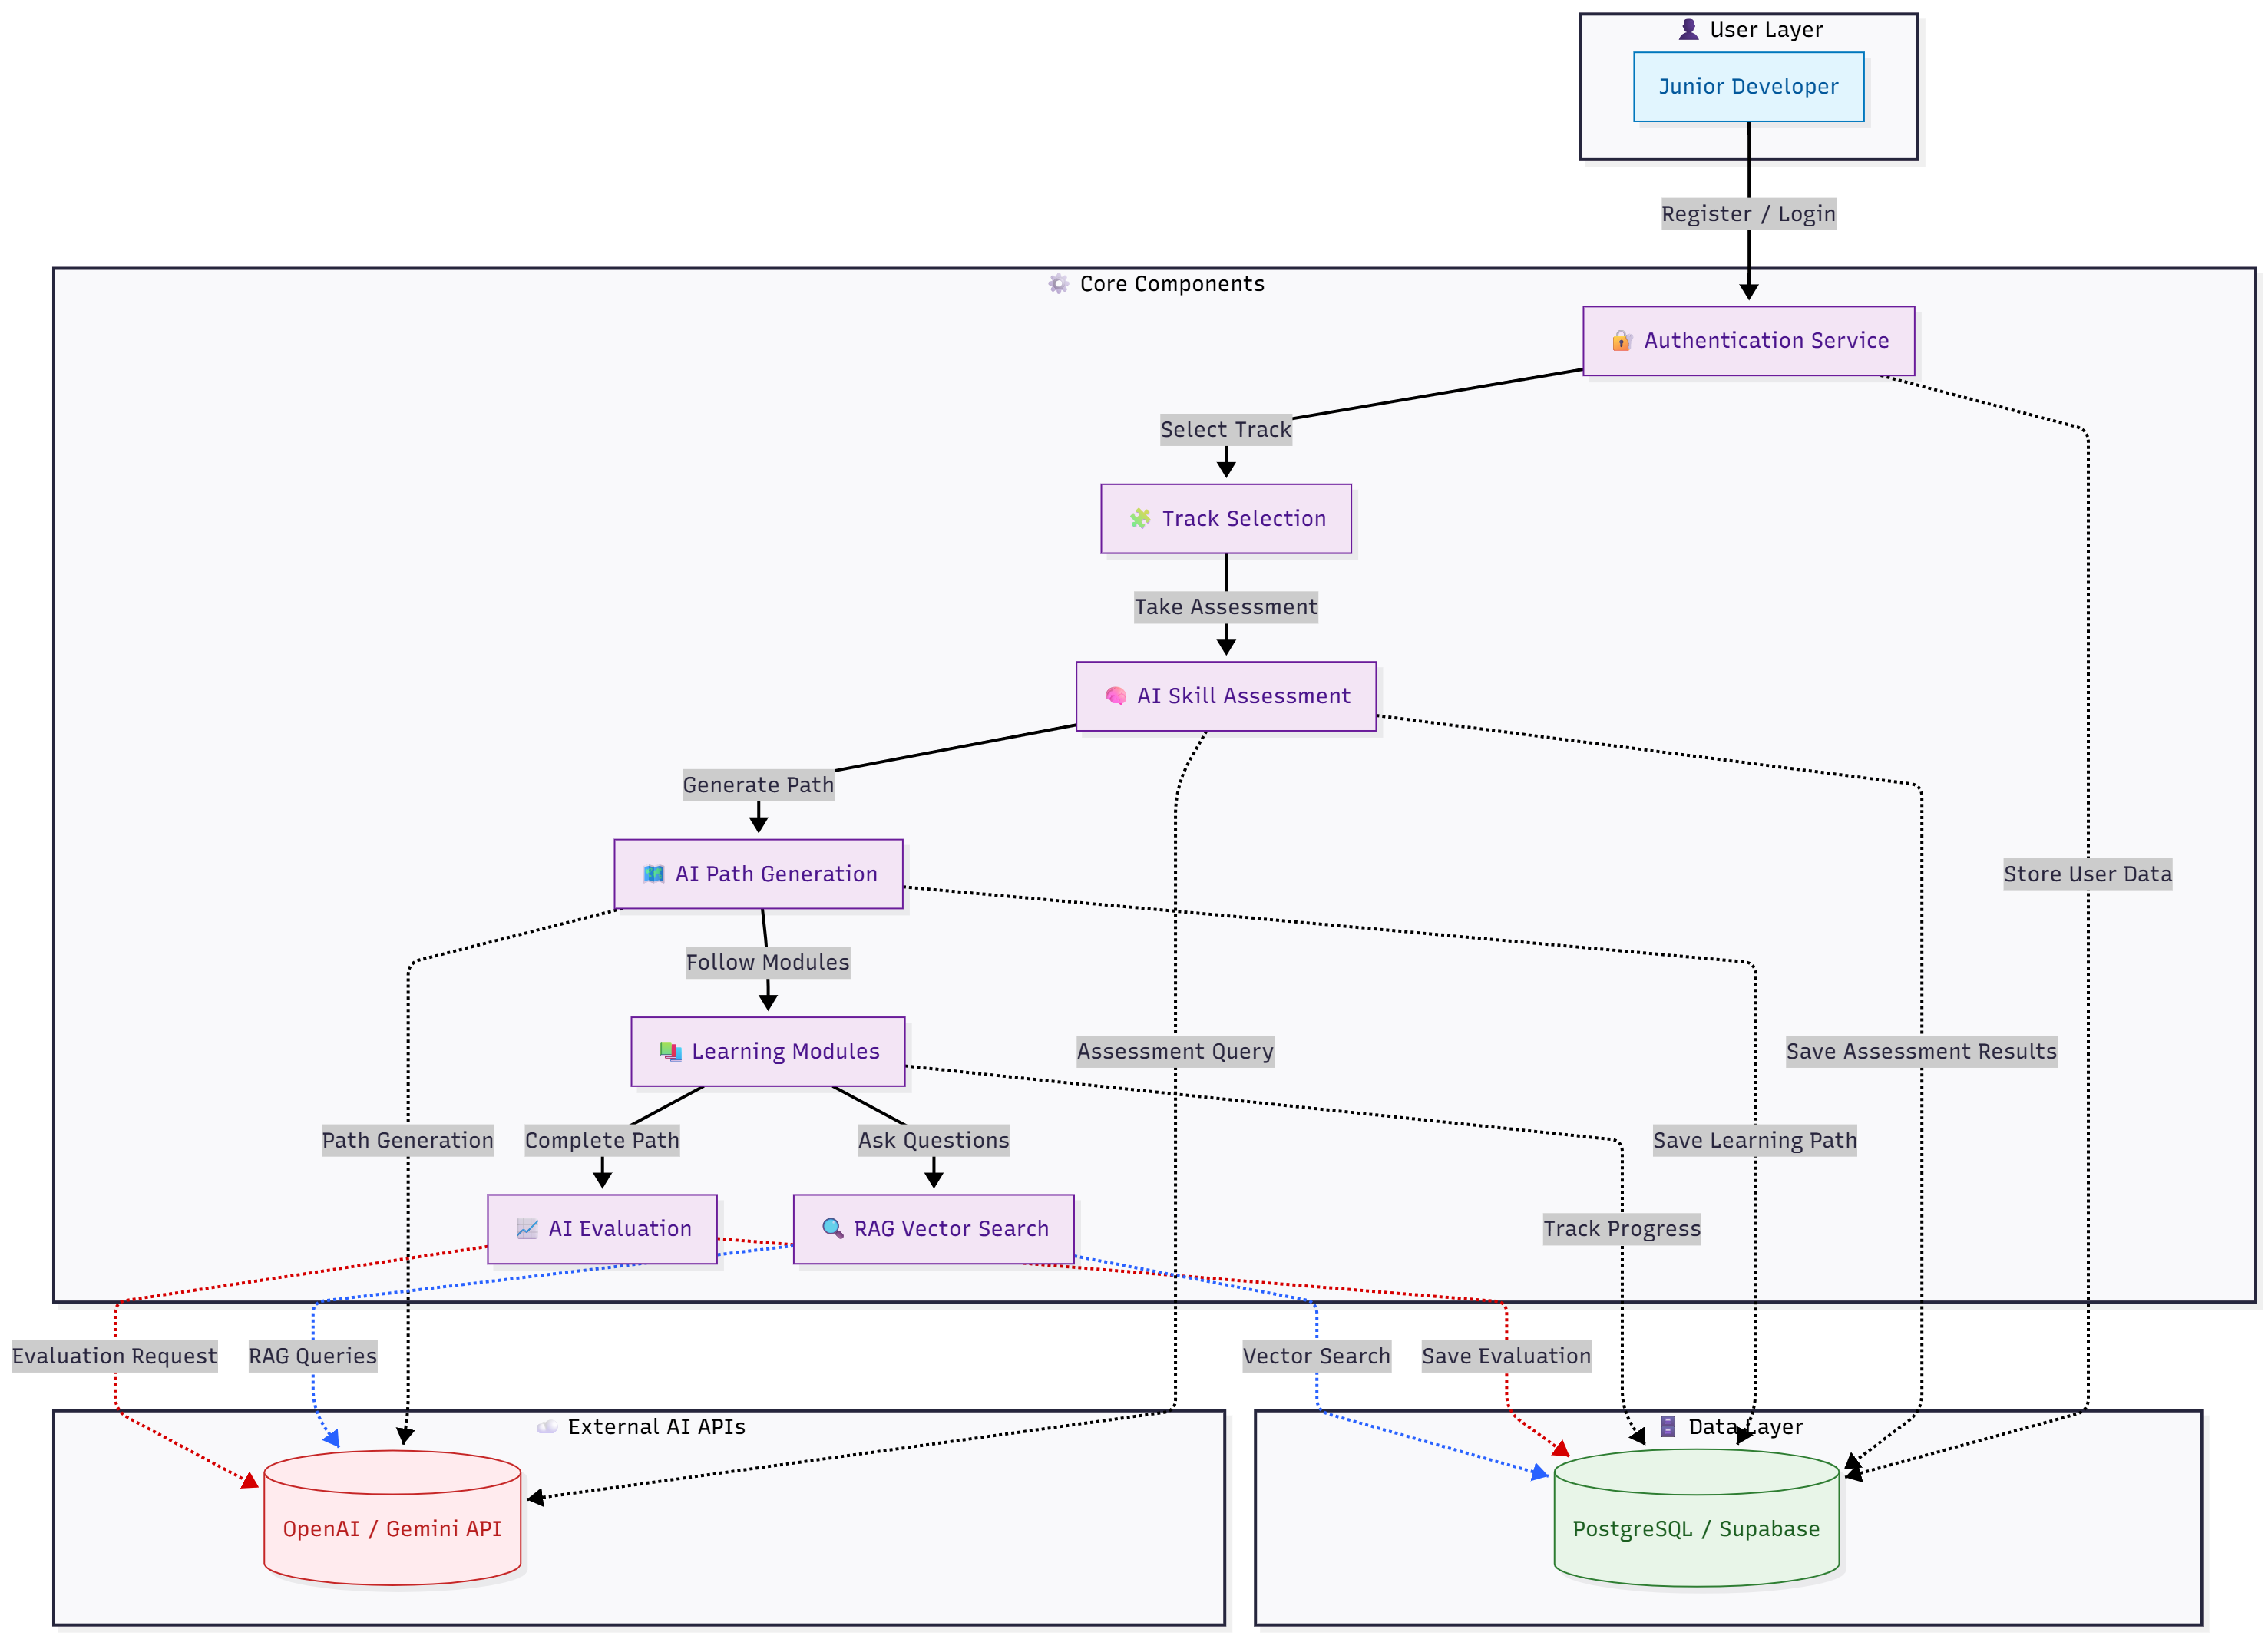
\includegraphics[width=0.95\textwidth]{Figures/arthitectural_structure.png}
    \caption{GrowWise architecture overview—showing interaction between frontend, backend, AI services, and database.}
    \label{fig:architecture}
\end{figure}


\subsection{High-Level System Decomposition}
The GrowWise platform breaks down into four main parts, each handling its own tasks:
\begin{itemize}
    \item User Interface Layer: Takes care of all interactions with users and offers an easy-to-use web interface
    \item Application Services Layer: Holds the main business rules and guides user activities
    \item AI Services Layer: Deals with all AI features like testing skills, creating learning plans, and checking progress
    \item Data Persistence Layer: Manages storing, getting, and organizing data
\end{itemize}
\subsection{Major System Responsibilities}
The software system needs to handle these main jobs:
\begin{enumerate}
    \item User Management: Safe login, profile handling, and keeping track of sessions
    \item Adaptive Learning: Checking user skills on the fly and making custom learning plans
    \item Content Delivery: Showing interactive lessons with built-in AI help
    \item Intelligent Evaluation: Using AI to review user progress and project work
    \item Progress Tracking: Keeping a full record and reports on how users are doing
    \item Administrative Control: Managing lesson content, paths, and system settings
\end{enumerate}
\subsection{Component Roles and Responsibilities}
\subsubsection{User Interface Layer}
\begin{itemize}
    \item Authentication Module: Handles logging in, signing up, and managing sessions
    \item Track Selection Interface: Lets users pick their area of focus for learning
    \item Assessment Interface: Shows tests for skill checks and gathers answers
    \item Learning Dashboard: Displays custom learning plans and tracks progress
    \item Module Interface: Offers an interactive space for learning with an AI chat built in
    \item Evaluation Interface: Allows submitting projects and showing feedback
\end{itemize}
\subsubsection{Application Services Layer}
\begin{itemize}
    \item User Service: Manages user accounts and login rules
    \item Assessment Service: Handles skill tests and scoring
    \item Path Generation Service: Builds custom learning maps
    \item Module Service: Takes care of delivering lessons and tracking progress
    \item Evaluation Service: Organizes AI reviews for projects
    \item Admin Service: Gives tools for admins to manage content
\end{itemize}
\subsubsection{AI Services Layer}
\begin{itemize}
    \item LLM Integration Service: Connects to outside AI services like OpenAI or Gemini
    \item RAG System: Uses retrieval to add context for better AI help
    \item Vector Database: Keeps and searches embeddings of learning materials
    \item Assessment AI: Reviews answers and gives skill scores
    \item Path Planning AI: Makes flexible learning plans based on user info
    \item Evaluation AI: Gives feedback like a senior engineer on projects
\end{itemize}
\subsubsection{Data Persistence Layer}
\begin{itemize}
    \item User Database: Stores user info, login details, and preferences
    \item Content Database: Handles lessons, paths, and learning resources
    \item Progress Database: Tracks how users are advancing, what's done, and performance
    \item Vector Store: Holds embeddings for quick content searches
    \item Session Storage: Manages short-term data and user sessions
\end{itemize}

\subsection{Component Collaboration and Data Flow}
The system components collaborate through well-defined interfaces and data flows:

\begin{enumerate}
    \item User Authentication Flow: Interface Layer → User Service → Database
    \item Assessment Process: Interface Layer → Assessment Service → AI Services → Database
    \item Path Generation: Assessment Service → Path Planning AI → Module Service
    \item Learning Process: Module Service → RAG System → Vector Database → AI Services
    \item Evaluation Process: Evaluation Service → Assessment AI → Database
\end{enumerate}

\subsection{Architectural Rationale}
This decomposition was chosen over alternative approaches for the following reasons:

\begin{itemize}
    \item Layered Architecture: Provides clear separation of concerns and maintainability
    \item Microservices Pattern: Enables independent scaling and deployment of AI services
    \item API-First Design: Facilitates integration with external AI providers and future extensions
    \item Stateless Services: Ensures scalability and fault tolerance
    \item Modular AI Integration: Allows easy switching between AI providers and models
\end{itemize}

Alternative monolithic approaches were rejected due to scalability limitations and tight coupling between AI and business logic components.

\subsection{External System Integration}
The system integrates with the following external services:

\begin{itemize}
    \item OpenAI/Gemini APIs: For LLM-based AI functionality
    \item AWS VPS: For hosting and infrastructure services
    \item Supabase: For database and authentication services
    \item Vector Database Services: For embedding storage and retrieval
\end{itemize}


\subsection{Subsystem Architecture}
The AI Services Layer is main part of system. It handle all smart AI thing by connect to outside API. It got many small part that work together make good learning.

\subsubsection{AI Assessment Module}
This module check user skill use outside AI API. It make question from path user choose and send answer to external AI check. It get back score and weak spot then save in database for make plan. All depend on external AI for make question and grade.

\subsubsection{AI Path Generation Module}
This module make special plan for every user with help from outside AI. It take test result and send to external API with user path. AI think and send back lesson order with step and goal. Then save plan in database so system can use.

\subsubsection{Learning Module with RAG}
This module give real learning with AI help from outside API. When user ask question or need help it send to external AI with lesson info. AI answer with good explain and tip. It also watch user progress and what they finish.

\subsubsection{AI Evaluation Module}
This module check user project use outside AI API. It send work and answer to external AI for look. AI give deep feedback, score and how to better. Like senior engineer talk, all from external AI.

\subsubsection{External API Integration}
All AI in system come from outside like OpenAI and Gemini. System call these API for test, plan, RAG help and project check. Every part handle own API talk, make request right, get answer and fix error. These API make system smart and fun.

\subsubsection{Data Flow}
User info go through AI layer, outside API do every step. Test answer go to API for score, plan request go to AI, help question in learning go to RAG external, project check by outside AI. All result save in local database for later and make system good.

\section{Architectural Strategies}
This part tell key choice we make for GrowWise design.

\subsection{Using External AI APIs}
We use outside AI like OpenAI and Gemini not make own AI. This way we get new AI easy no train hard. No need fix model or update ourself. Pay only when use so money save.
Make own model too expensive and hard. Use external let us focus on learning app not AI.

\subsection{Using RAG for Smart Help}
We use RAG mean Retrieval-Augmented Generation for give learner good help. It take info from database and mix with AI for answer. This keep help new and right, no need update hand.
Old fix page too boring and hard maintain. RAG give what need right time.

\subsection{Choosing Modern Technology}
We pick new tool like Next.js for front, FastAPI for back, PostgreSQL for data. These good with AI and easy use. Make platform fast and strong.
Old tech slow and hard connect AI. New choice make build quick.

\subsection{Using Microservices}
We make system small separate service that talk each other. This let us change one without break all. If one problem other still work.
Make system strong and easy handle.

\subsection{API-First Design}
We build everything with API first. This easy connect outside AI and add new thing later. Can make mobile app or connect other system.
This way platform can change and ready for future.

\section{Domain Model/Class Diagram}
The domain model and class diagram show full how GrowWise build. It show main part, what they have, what they do and how connect. Setup split three view that help each other, each look different side how system work.
View 1: User Journey \& Progress talk how learner go through system. From sign up pick path, check skill, make plan, track progress and get report. This show user flow and how system change from result.
View 2: AI Services \& Knowledge Management show smart part for personal learning. Got RAG knowledge with vector, AI mentor for talk, path maker for plan change, RAG helper for lesson help.
View 3: Project Workflow \& Evaluation tell process for task and check. Show how project give to user, how submit and check by AI like engineer, feedback help better. This stress learn by real way and solve true problem.
All view together show full GrowWise, how data move, user do, and AI fit good for personal learning.

\begin{figure}[!h]
    \centering
    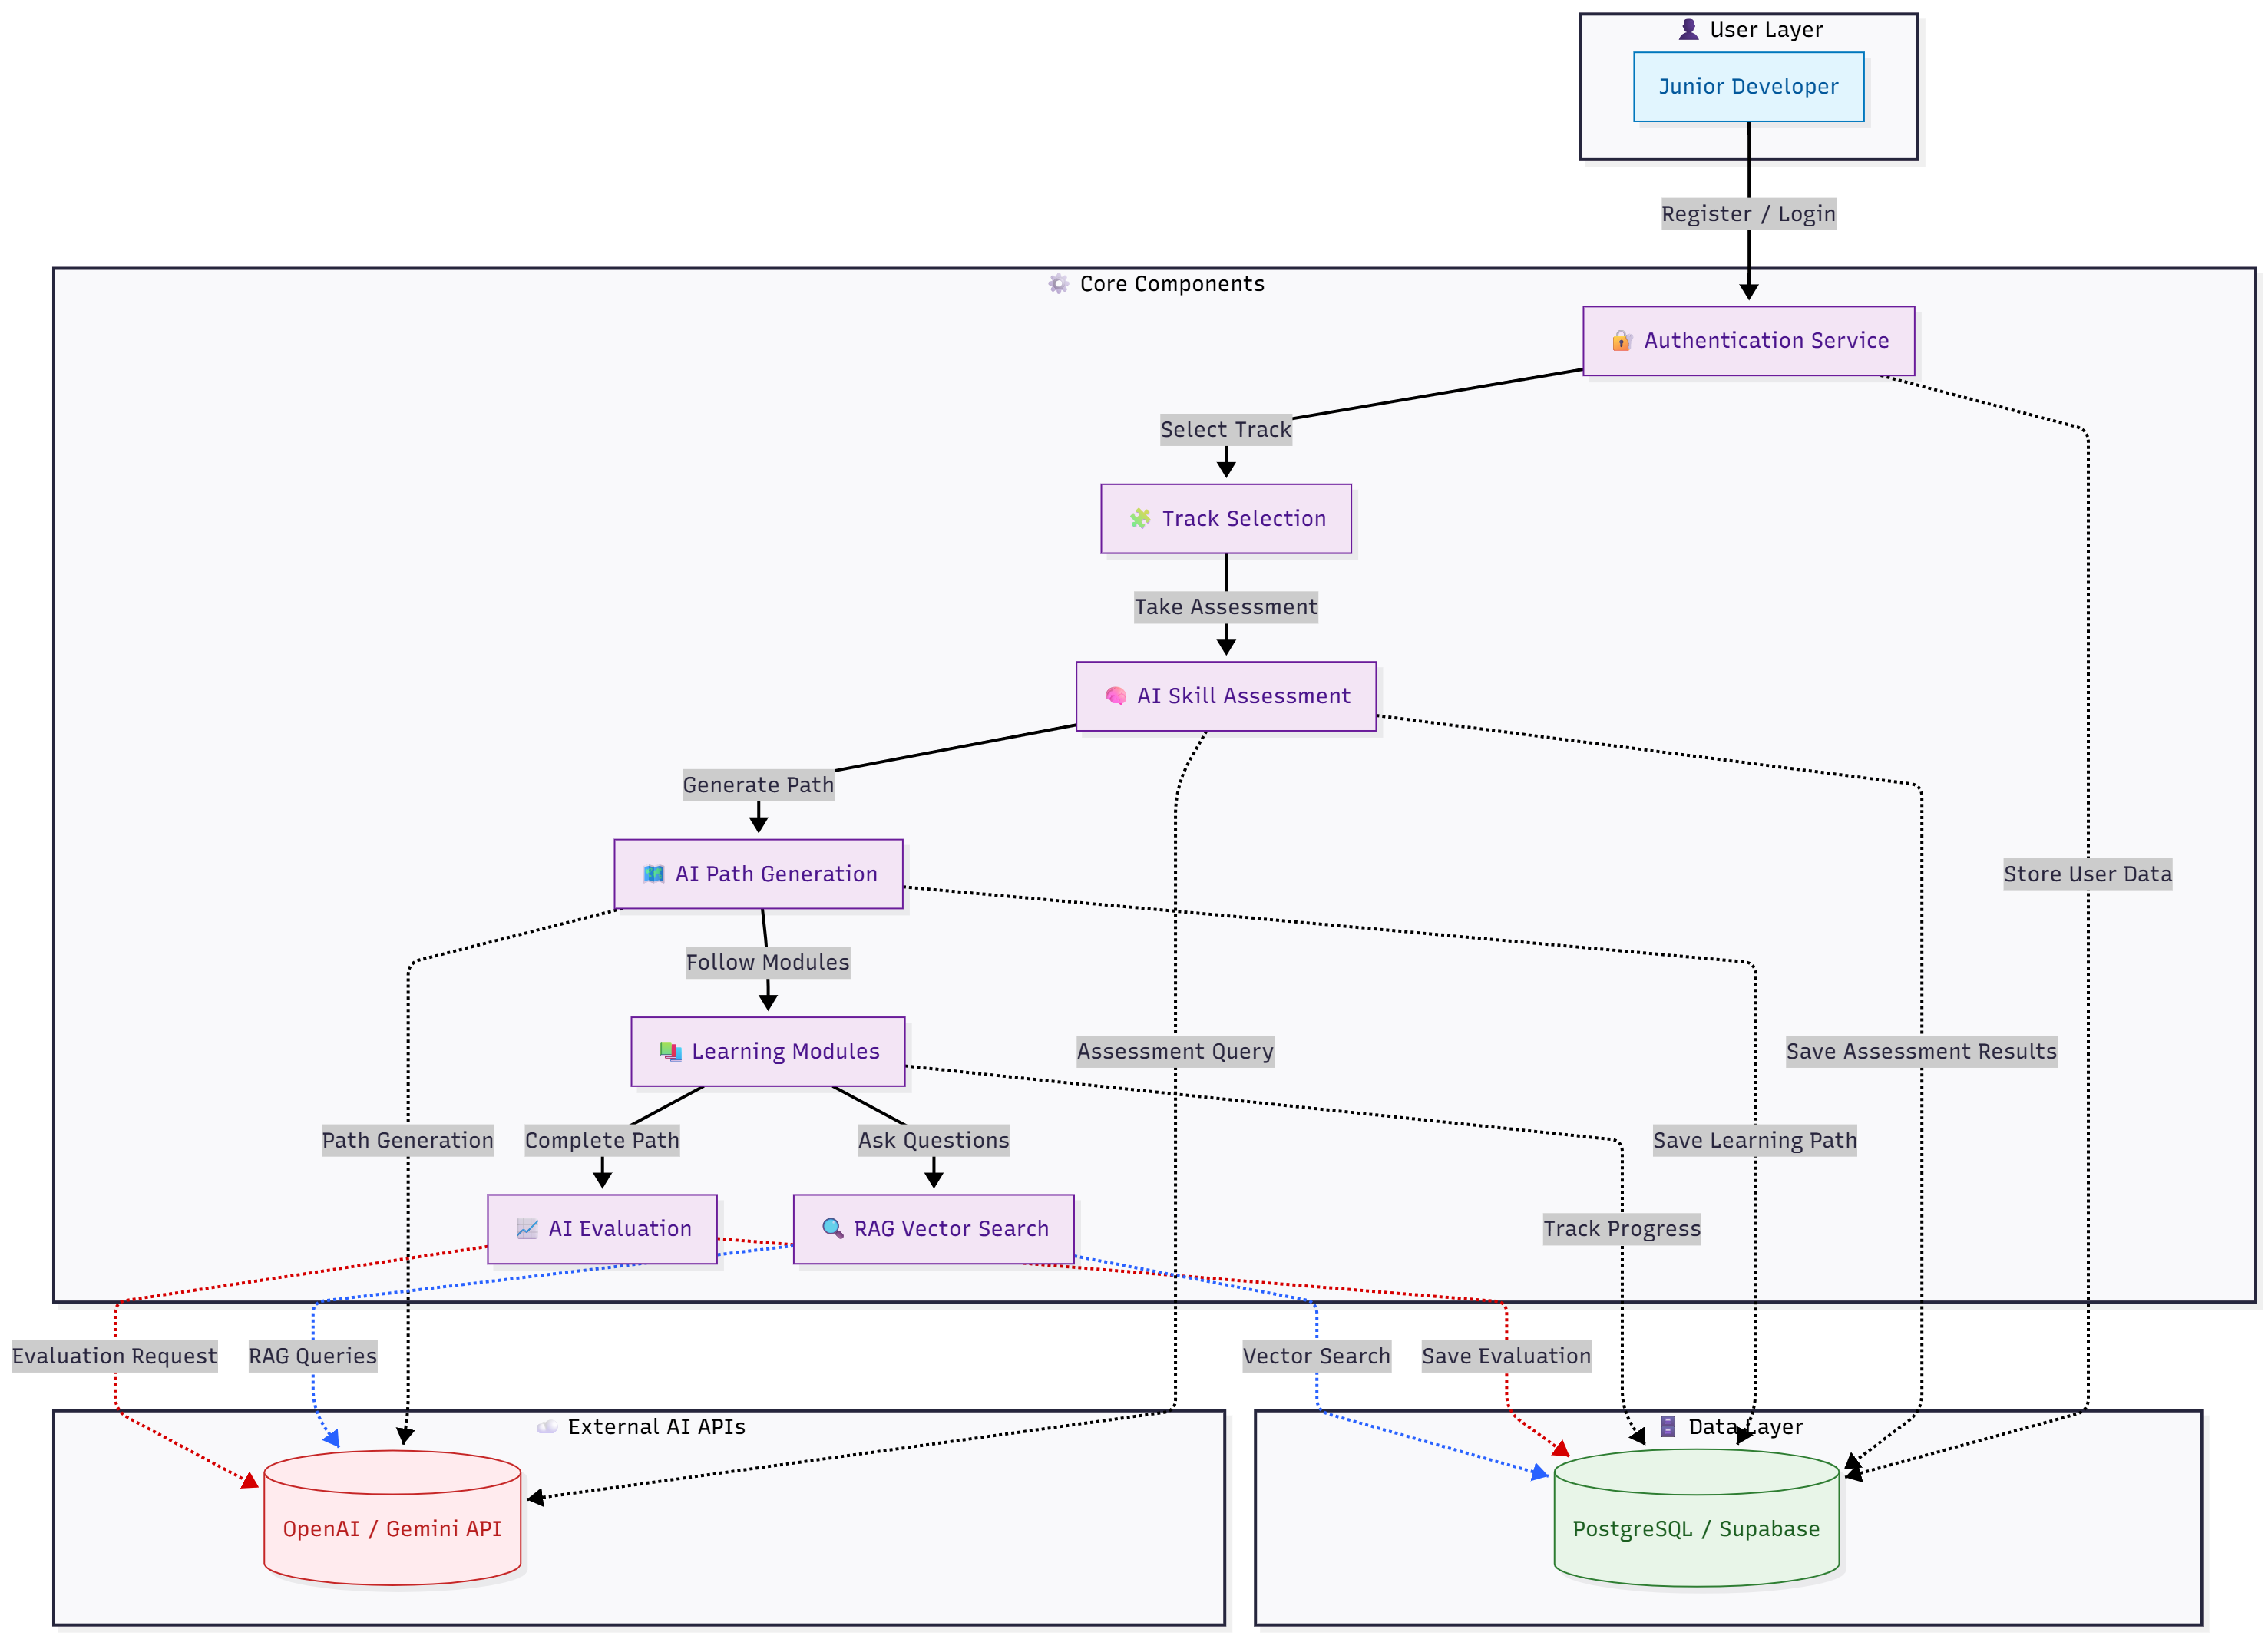
\includegraphics[width=0.95\textwidth]{Figures/arthitectural_structure.png}
    \caption{GrowWise system architecture: frontend, backend, AI, and database.}
    \label{fig:architecture}
\end{figure}

\begin{figure}[H]
    \centering
    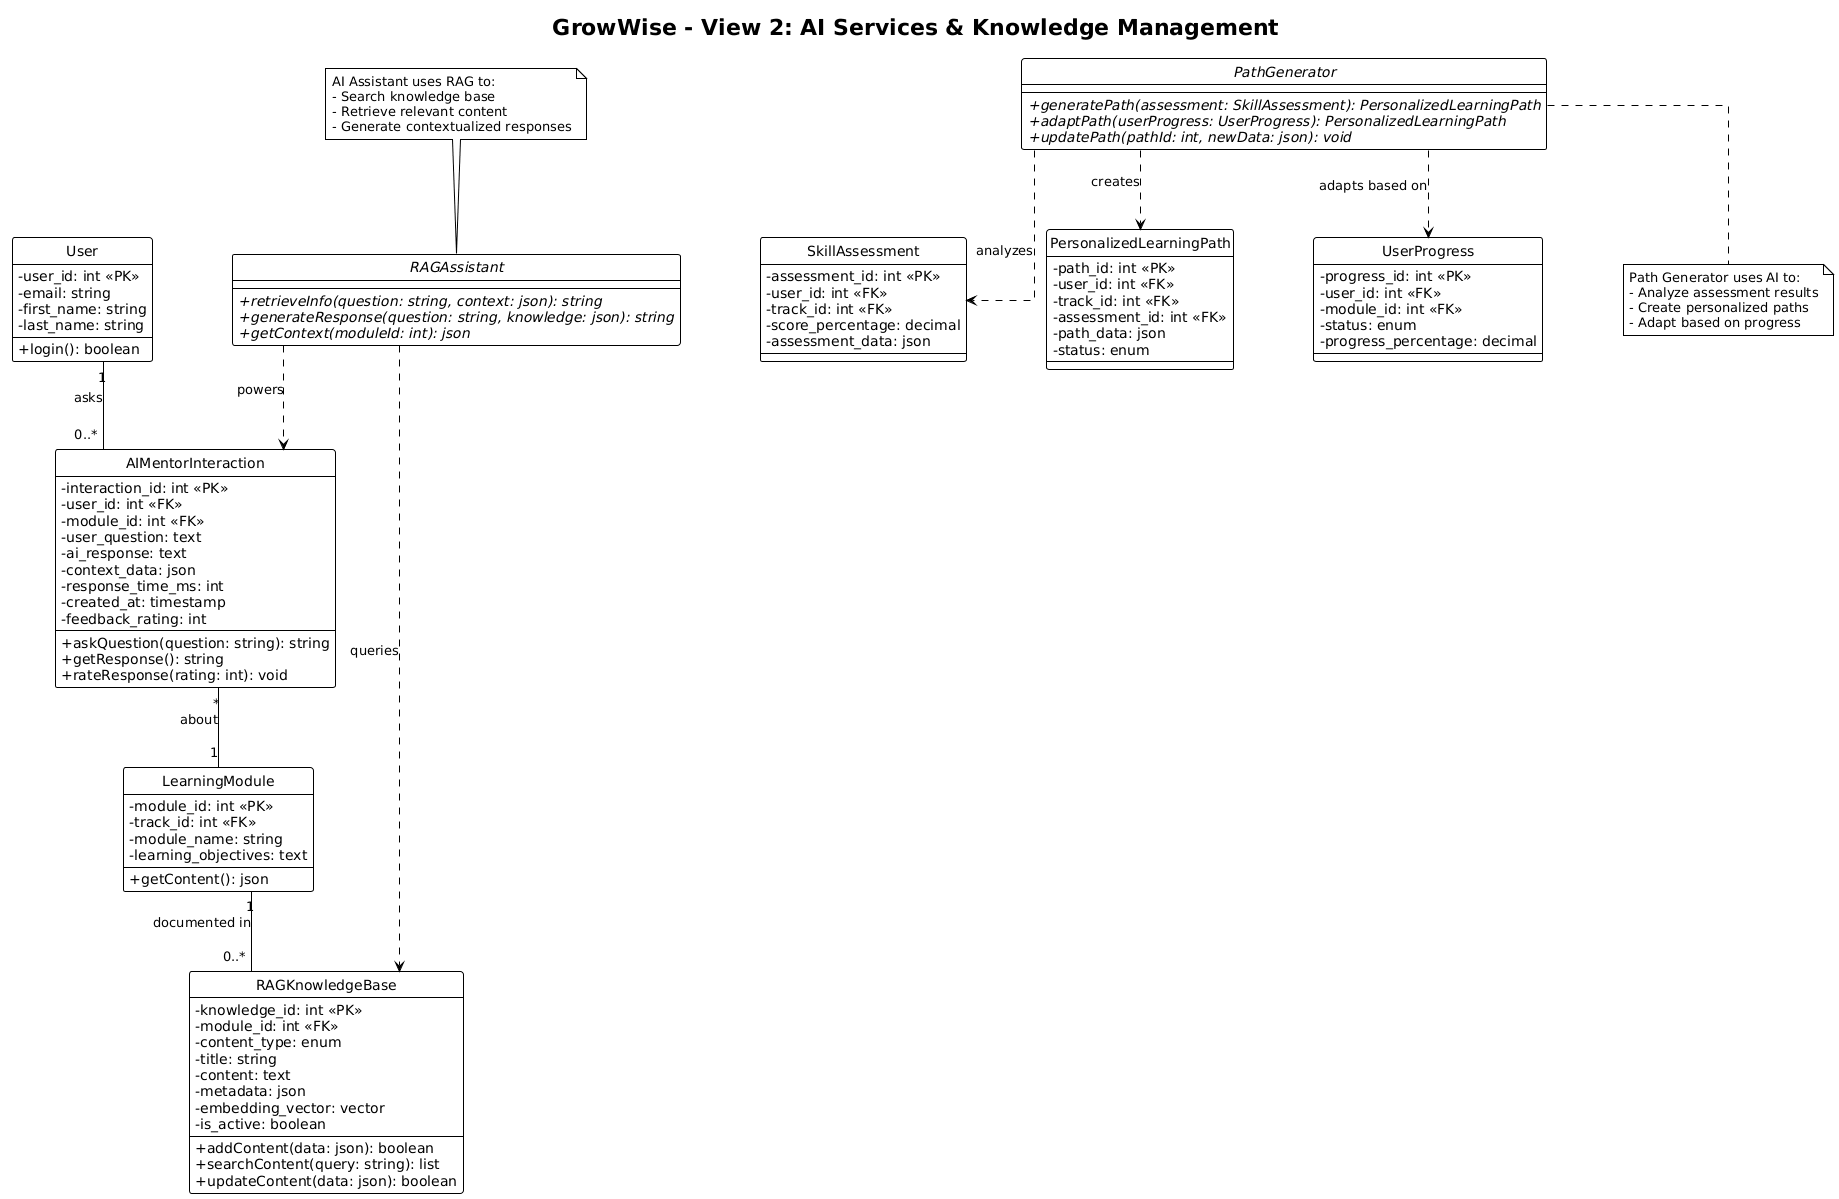
\includegraphics[width=\textwidth]{Figures/Diagram2.png}
    \caption{GrowWise – View 2: AI Services \& Knowledge Management, highlighting components like the RAG knowledge base, contextual assistant, path generator, and AI mentor for adaptive, context-aware learning.}
    \label{fig:class_diagram_view2}
\end{figure}

\begin{figure}[H]
    \centering
    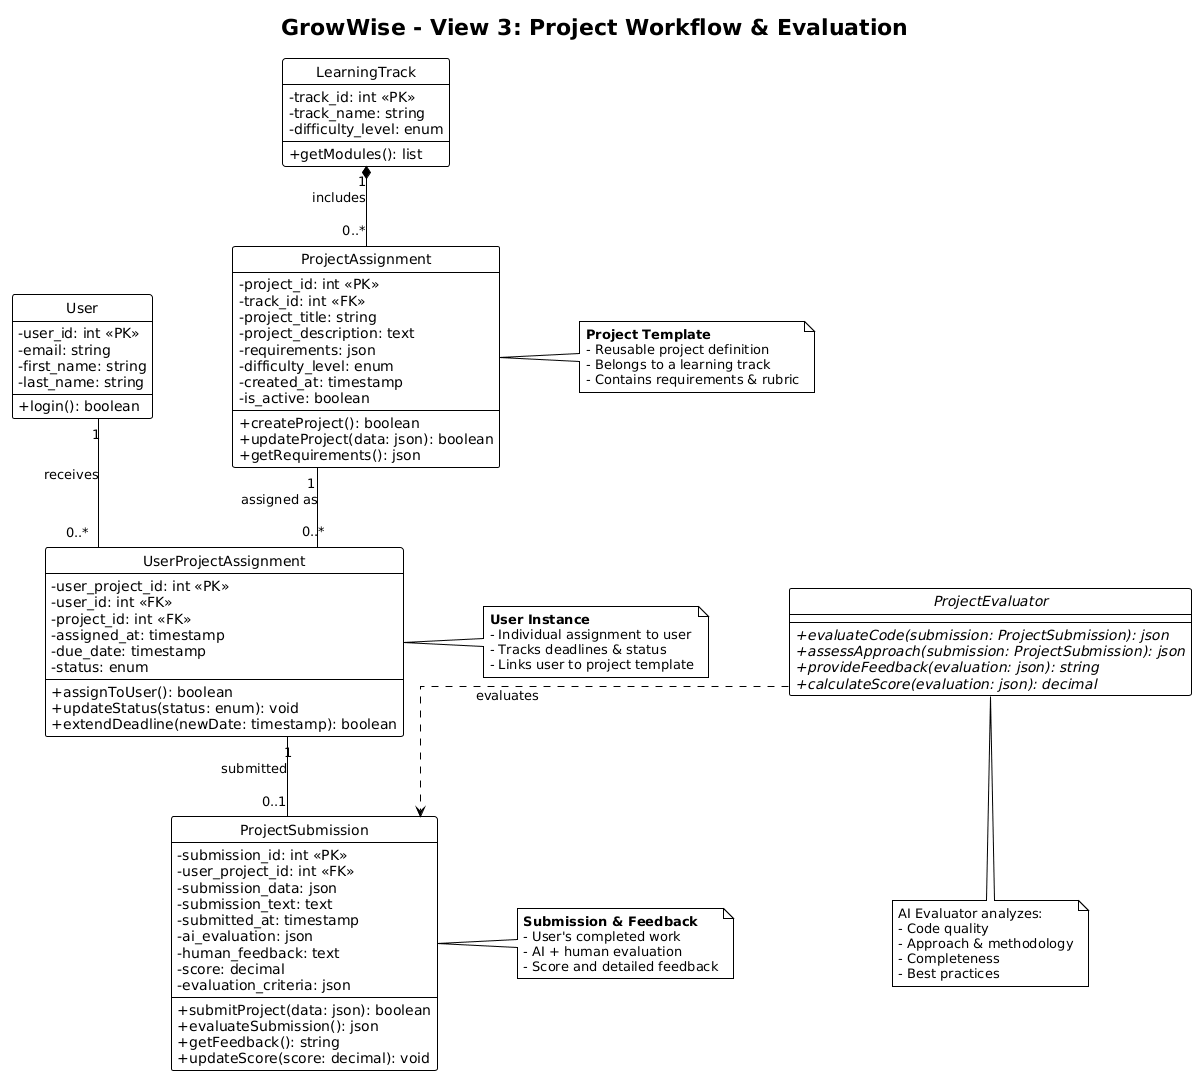
\includegraphics[width=\textwidth]{Figures/Diagram3.png}
    \caption{GrowWise – View 3: Project Workflow \& Evaluation, showing how projects are assigned, submitted, and AI-evaluated with scoring and feedback.}
    \label{fig:class_diagram_view3}
\end{figure}

\section{Policies and Tactics}
This section explains the exact design decisions and the implementation aspects that influence the work of the system.
\subsection{Codebase Organization}
Our code is well-organised in a simple folder structure. The primary project is divided into three major folders: frontend that contains the user-facing aspects, backend which contains server-related aspects, and shared which contains code which is shared between the two ends.
We put similar files together just in the same folder. Similar, all of the code relating to logins in a single location, all lesson module code in a different location. In this manner, it is easy to locate things and update them.
We use a regular name of folders and files. Folders are small case with the use of underscores and files are similar to that. It assists in all getting the layout quickly.
\subsection{Development Tools}
We select specific instruments in constructing the application. VS Code is the primary choice of everyone because it is compatible with our languages. The version tracking is done by Git and the code is stored in GitHub.
Docker deploys the app on local computers and in live environments to ensure that environments remain similar. The APIs are tested by Postman and the front end is debugged using Chrome DevTools.
We also record everything so that new members can be on their feet fast. And automatic install and set up scripts.
\subsection{Coding Guidelines}
We possess simple coding regulations. Code must be well maintained and understandable. Instruments auto-make it appear homogenous.
Classes and functions are assigned meaningful names. We add notes for tricky parts. In Python, type hints are used to explain things.
Code before merge is auto checked to be compliant to rules.
\subsection{Testing Strategies}
There are various ways of testing code. Unit tests are analyzed of individual functions, the integration tests of how components are linked together and end-to-end tests of the complete user paths.
Tests are made of new features and fixes. They have to die before they can unite. We monitor the extent of code tests and are ambitious.
Automated applications will perform tests on all the changes and this will ensure that things are always working and that any problems are identified early.
\subsection{Documentation Practices}
We document everything well. The APIs receive clear definitions on the uses and how they work. Complex bits have code notes.
We maintain platform user guides and dev guides of the code. In addition, deployment instructions and troubleshooting manuals.
We update documentations with the changes and go through them regularly to ensure that they are accurate and useful.
\section{Conclusion}
This chapter provided a complete design specification of the GrowWise AI-based adaptive learning platform, including overall decisions and construction plans. It began with an in-depth analysis of what the system requires and constrains which resulted in a scalable, expandable structure that addresses the difficulties in teaching developers. The proposed architecture consists of the latest technologies, such as Next.js as the front, FastAPI as the back-end services, PostgreSQL as the database, and AI APIs, as the intelligent path generator, and verification. It is based on learning approaches, where path making on the fly, AI guidance in real-time (through RAG) knowledge pulls, and complete checks analysing the skills as well as problem-solving methods are considered. The decisions are made according to growth, ease of maintenance and user feel and address security, speed and access needs. The modular design enables the part of the building and testing to be made in isolation, which can be improved and added easily. The comprehensive documentation, including class schema, system connections, and construction architecture provide a good groundwork to develop on. The design addresses the primary objectives of a bespoke, flexible platform that transcends predetermined courses in order to provide dynamic systems that are conscious and tailored to the requirements and learning styles of every developer.
\chapter{Implementation and Testing}
The chapter addresses the process of creating and testing the GrowWise prototype. It contains the technology selections, determining the particulars of the keybuilds of the parts, the connections with AI, data archives, test arrangement, and test results, launch, and present constraints.
\section{Implementation}
The following are the construction specifications of the components and procedures of the plan.
\subsection{Learning Track and Module System}
The Learning Track and Module System establishes the framework of the simple system of GrowWise, with lessons arranged into definite sequences. Big tech areas are referred to as tracks and modules are the units within the tracks.
To begin with, we have created a flexible database structure consisting of multitrack and ordered modules. The back end is a FastAPI SQLAlchemy based implementation of LearningTrack and LearningModule items. Songs are listed on a table named, described, difficulty, and time estimate. Tracks are interconnected through a key to a module and order exists.
The next.js and React front end display tracks in cards which contain information such as description, difficulty, and time. The selection of a track stores a UserTrackSelection link. The module view presents information sequentially with text, videos, coding assignments, and quizzes. It verifies requirements to maintain the appropriate sequence.
Modules are loaded depending on the user spot in the path. UserProgress in progress tracks including status, time and percent. Admins have the ability to revise content without discontinuing progress, quality versions.
\subsection{AI-Powered Skill Assessment Module}
The AI-Powered Skill Assessment Module tests to determine user knowledge and problem-solving to identify the optimal start. It combines smart grading with AI generated questions.
The track is made by using outside AI APIs such as OpenAI or Gemini to make questions. The back end receives track information, constructs a prompt that the AI will use to generate questions on knowledge and methods. It establishes types, problems and coverage.
There are questions that have options of facts, reasoning questions, and practice questions in terms of their coding. Every save has its track, difficulty and criteria. We retain a bank to be reused, and make others to personal checks.
In grading, questions and answers are submitted to the AI using back end with the prompt to verify the correctness, reasoning and understanding. It identifies areas of weaknesses, strengths, and provides feedback on techniques.
Scores, JSON, and time of results are stored in SkillAssessment. AI information informs the decisions of making a path, closing holes, and creating strengths.
\subsection{AI Learning Path Generation Module}
The AI Learning Path Generation Module creates personalized road maps based on the assessments and creates the order of the best modules. It encompasses information analysis and artificial intelligence design.
It starts after assessment. Results such as scores, gaps, strengths and track are obtained through back end. This passes on to AI with module data, requirements, challenges, and objectives.
AI is the planner based on immediate information on the user, modules, connections and regulations. It tracks a route using systematized modules, areas of focus, times and milestones.
Path It is a JSON containing module IDs, positions, prerequisites, times and objectives. It consists of adaptive features such as reviews, additional practice and advanced options.
It Stores the PersonalizedLearningPath as a flexible JSON file. UserProgress System watches move forward in the path, performance check, and makes the path refined with AI when necessary.
It monitors progress, speed and problem areas. Massive alterations cause path updates to align with actual learning.
Path is displayed as interactive map on front end where the nodes represent modules and display the status. It has used percent, time remaining and milestones. Position, links, and module details are displayed to the users.

\subsection{RAG Implementation for Integrated Learning Sources Context}
The Retrieval-Augmented Generation (RAG) system is developed on the lines of the smart system that retrieves learning materials to form a knowledge base rich in context. This allows the AI mentor to offer precise and useful guidance in terms of well-selected educational content. This was constructed in a stepwise fashion that manages materials, constructs semantic embeddings, and mining out pertinent content intelligently.
It begins with content importation, during which we collect information such as documentation, tutorials, code snippets, explanations and documentation and prepare it. The back end contains uploading file, picking type and linking to modules administrative tool. It works with PDF, markdown, text and JSON.
The processing is a breaking down of docs into meaningful pieces. We cut smartly, but we still keep structure structured such as paragraphs, headers, code, sentences, etc. as opposed to cutting by size.
Every work is converted to embeddings with the models of OpenAI such as text-embedding-ada-002 to obtain vectors that encode the meaning. This facilitates the process of locating the related concepts, not only the identical words.
To enable us to find the vectors quickly in the database, we use PostgreSQL and pgvector. The pieces are stored in the RAGKnowledgeBase with their vectors, source information, type, link to a module, and some time. Indexes also enable rapid searches with large quantities of data.
Retrieval combines semantic search and filters. In the case of user query, we embed the query, and find similar vectors by cosine. We are able to narrow down to the module or type.
We prioritize the best pieces, take the most few such as 3-5 and submit them along with the question to the LLM. The prompt will direct the AI to apply that information to give precise and cordial responses such as a mentor.
We made our adjustments towards enhanced speed and precision. Caching is the records of frequent questions and descriptions so as to reduce the number of calls and accelerate the process and time-outs are used to refresh it. We extend queries with module background and user history also.
All the mentor chats are logged in AIMentorInteraction, including the question, chunks, response, time and feedback. This assists in identifying patterns, missing knowledge and enhancing retrieval.
Each module of the front end possesses a smooth chat that displays history, indicates natural questions and clear responses. It proposes questions, displays content that is referred to, and allows users to rate responses.
\subsection{AI Evaluation Module}
After successfully going through each module and its content, we implemented a Gemini-based chatbot AI evaluator. It has complete context about the track, user journey, and the educational content the user has consumed and studied.After that, the AI works like a reverse ChatGPT, asking the user questions through a chatbot. Once the session ends, it provides a complete progress report to the end user. In this report, it clearly shows the user’s level when they started and what their current level is now.



\section{Test case Design and description}

This section presents the test cases designed and executed for each major functional module of the GrowWise platform. Common shared attributes across all test cases are: a modern web browser with JavaScript enabled, the FastAPI backend running on the configured port, a PostgreSQL database connected, and internet access for AI API calls. Each test case follows the standardised format and was verified against the fully implemented system.

% ----------------------------------------------------------------
% TC-AUTH-01
% ----------------------------------------------------------------
\begin{table}[H]
\footnotesize
\centering
\caption{Test Case TC-AUTH-01: User Login Authentication}
\label{tab:tcauth}
\begin{tabular}{|p{2.5cm}|p{4cm}|p{2.5cm}|p{4.5cm}|}
\hline
\multicolumn{4}{|c|}{\textbf{Authentication \& Account Security Module}} \\ \hline
\multicolumn{4}{|c|}{\textbf{GrowWise v1.0 -- server/app/routers/auth.py}} \\ \hline
\textbf{Test Case ID:} & TC-AUTH-01 & \textbf{QA Test Engineer:} & M. Umair Imran \\ \hline
\textbf{Test case Version:} & 1.0 & \textbf{Reviewed By:} & Maryam Nasim \\ \hline
\textbf{Test Date:} & 10/03/2026 & \textbf{Use Case Ref:} & UC-01 User Login \\ \hline
\textbf{Revision History:} & \multicolumn{3}{p{11cm}|}{No prior revision history.} \\ \hline
\textbf{Objective:} & \multicolumn{3}{p{11cm}|}{Verify a registered user can log in with valid credentials and receive a JWT access token.} \\ \hline
\textbf{Product/Ver/ Module:} & \multicolumn{3}{p{11cm}|}{GrowWise v1.0 / Authentication Module} \\ \hline
\textbf{Environment:} & \multicolumn{3}{p{11cm}|}{Web browser, FastAPI backend, PostgreSQL, Python 3.10+, Node.js 18+} \\ \hline
\textbf{Assumptions:} & \multicolumn{3}{p{11cm}|}{User account exists in the database. Backend server is running.} \\ \hline
\textbf{Pre-Requisite:} & \multicolumn{3}{p{11cm}|}{A registered user account with a valid email and password must exist.} \\ \hline
\textbf{Step No.} & \textbf{Execution Description} & \multicolumn{2}{p{7cm}|}{\textbf{Procedure Result}} \\ \hline
1 & User navigates to the login page. & \multicolumn{2}{p{7cm}|}{Login form displays email and password input fields.} \\ \hline
2 & User enters valid credentials and clicks Submit. & \multicolumn{2}{p{7cm}|}{System validates credentials and issues JWT access and refresh tokens.} \\ \hline
3 & System redirects user to the dashboard. & \multicolumn{2}{p{7cm}|}{Dashboard loads with the authenticated user profile data.} \\ \hline
3-A & User enters an incorrect password. & \multicolumn{2}{p{7cm}|}{System shows ``Incorrect email or password'' error message.} \\ \hline
\multicolumn{4}{|p{13.5cm}|}{\textbf{Comments:} Both valid and invalid credential flows tested and verified.} \\ \hline
\multicolumn{4}{|c|}{\underline{\textbf{Passed}} \quad\quad\quad Failed \quad\quad\quad Not Executed} \\ \hline
\end{tabular}
\end{table}

\vspace{0.5em}

% ----------------------------------------------------------------
% TC-TRACK-01
% ----------------------------------------------------------------
\begin{table}[H]
\footnotesize
\centering
\caption{Test Case TC-TRACK-01: Learning Track Selection}
\label{tab:tctrack}
\begin{tabular}{|p{2.5cm}|p{4cm}|p{2.5cm}|p{4.5cm}|}
\hline
\multicolumn{4}{|c|}{\textbf{Track Selection Module}} \\ \hline
\multicolumn{4}{|c|}{\textbf{GrowWise v1.0 -- server/app/routers/tracks.py}} \\ \hline
\textbf{Test Case ID:} & TC-TRACK-01 & \textbf{QA Test Engineer:} & M. Shahzad Waris \\ \hline
\textbf{Test case Version:} & 1.0 & \textbf{Reviewed By:} & Maryam Nasim \\ \hline
\textbf{Test Date:} & 10/03/2026 & \textbf{Use Case Ref:} & UC-02 Track Selection \\ \hline
\textbf{Revision History:} & \multicolumn{3}{p{11cm}|}{No prior revision history.} \\ \hline
\textbf{Objective:} & \multicolumn{3}{p{11cm}|}{Verify user can browse available learning tracks and select one to begin personalized learning.} \\ \hline
\textbf{Product/Ver/ Module:} & \multicolumn{3}{p{11cm}|}{GrowWise v1.0 / Track Selection Module} \\ \hline
\textbf{Environment:} & \multicolumn{3}{p{11cm}|}{Web browser, FastAPI backend, PostgreSQL database, Python 3.10+} \\ \hline
\textbf{Assumptions:} & \multicolumn{3}{p{11cm}|}{User is authenticated. At least one learning track exists in the database.} \\ \hline
\textbf{Pre-Requisite:} & \multicolumn{3}{p{11cm}|}{User must be logged in. Tracks must be available in the system.} \\ \hline
\textbf{Step No.} & \textbf{Execution Description} & \multicolumn{2}{p{7cm}|}{\textbf{Procedure Result}} \\ \hline
1 & User navigates to the track selection page. & \multicolumn{2}{p{7cm}|}{Available learning tracks displayed as selectable cards.} \\ \hline
2 & User selects a learning track (e.g., Web Dev). & \multicolumn{2}{p{7cm}|}{Track saved to UserTrackSelection table. Confirmation displayed.} \\ \hline
3 & System redirects to the skill assessment. & \multicolumn{2}{p{7cm}|}{User routed to assessment page for the chosen track.} \\ \hline
3-A & User proceeds without selecting any track. & \multicolumn{2}{p{7cm}|}{System prompts: ``Please select a track to continue''.} \\ \hline
\multicolumn{4}{|p{13.5cm}|}{\textbf{Comments:} Correct track saved to database and assessment session correctly initiated.} \\ \hline
\multicolumn{4}{|c|}{\underline{\textbf{Passed}} \quad\quad\quad Failed \quad\quad\quad Not Executed} \\ \hline
\end{tabular}
\end{table}

\vspace{0.5em}

% ----------------------------------------------------------------
% TC-ASSESS-01
% ----------------------------------------------------------------
\begin{table}[H]
\footnotesize
\centering
\caption{Test Case TC-ASSESS-01: AI Skill Assessment}
\label{tab:tcassess}
\begin{tabular}{|p{2.5cm}|p{4cm}|p{2.5cm}|p{4.5cm}|}
\hline
\multicolumn{4}{|c|}{\textbf{AI Skill Assessment Module}} \\ \hline
\multicolumn{4}{|c|}{\textbf{GrowWise v1.0 -- server/app/routers/assessment.py}} \\ \hline
\textbf{Test Case ID:} & TC-ASSESS-01 & \textbf{QA Test Engineer:} & Ameer Tufail \\ \hline
\textbf{Test case Version:} & 1.0 & \textbf{Reviewed By:} & Maryam Nasim \\ \hline
\textbf{Test Date:} & 11/03/2026 & \textbf{Use Case Ref:} & UC-03 Skill Assessment \\ \hline
\textbf{Revision History:} & \multicolumn{3}{p{11cm}|}{No prior revision history.} \\ \hline
\textbf{Objective:} & \multicolumn{3}{p{11cm}|}{Verify AI generates track-specific questions and evaluates answers to produce a skill score and learning path.} \\ \hline
\textbf{Product/Ver/ Module:} & \multicolumn{3}{p{11cm}|}{GrowWise v1.0 / AI Skill Assessment Module} \\ \hline
\textbf{Environment:} & \multicolumn{3}{p{11cm}|}{Web browser, FastAPI, Gemini/OpenAI API, PostgreSQL database} \\ \hline
\textbf{Assumptions:} & \multicolumn{3}{p{11cm}|}{Learning track is selected. AI API is accessible. Mock AI flag is disabled.} \\ \hline
\textbf{Pre-Requisite:} & \multicolumn{3}{p{11cm}|}{User must have a selected learning track before starting the assessment.} \\ \hline
\textbf{Step No.} & \textbf{Execution Description} & \multicolumn{2}{p{7cm}|}{\textbf{Procedure Result}} \\ \hline
1 & System creates an assessment session. & \multicolumn{2}{p{7cm}|}{10 AI-generated questions returned and displayed to the user.} \\ \hline
2 & User answers all questions and submits. & \multicolumn{2}{p{7cm}|}{Answers saved to the assessment responses table in the database.} \\ \hline
3 & User clicks Complete Assessment. & \multicolumn{2}{p{7cm}|}{AI batch-evaluates; skill score, report, and learning path generated.} \\ \hline
3-A & User attempts to complete with unanswered questions. & \multicolumn{2}{p{7cm}|}{System prompts user to answer all remaining questions first.} \\ \hline
\multicolumn{4}{|p{13.5cm}|}{\textbf{Comments:} AI response quality and mock fallback mode both tested and verified.} \\ \hline
\multicolumn{4}{|c|}{\underline{\textbf{Passed}} \quad\quad\quad Failed \quad\quad\quad Not Executed} \\ \hline
\end{tabular}
\end{table}

\vspace{0.5em}

% ----------------------------------------------------------------
% TC-LPATH-01
% ----------------------------------------------------------------
\begin{table}[H]
\footnotesize
\centering
\caption{Test Case TC-LPATH-01: AI Learning Path Generation}
\label{tab:tclpath}
\begin{tabular}{|p{2.5cm}|p{4cm}|p{2.5cm}|p{4.5cm}|}
\hline
\multicolumn{4}{|c|}{\textbf{AI Learning Path \& Stage Management Module}} \\ \hline
\multicolumn{4}{|c|}{\textbf{GrowWise v1.0 -- server/app/routers/learning.py}} \\ \hline
\textbf{Test Case ID:} & TC-LPATH-01 & \textbf{QA Test Engineer:} & M. Umair Imran \\ \hline
\textbf{Test case Version:} & 1.0 & \textbf{Reviewed By:} & Maryam Nasim \\ \hline
\textbf{Test Date:} & 11/03/2026 & \textbf{Use Case Ref:} & UC-04 Path Generation \\ \hline
\textbf{Revision History:} & \multicolumn{3}{p{11cm}|}{No prior revision history.} \\ \hline
\textbf{Objective:} & \multicolumn{3}{p{11cm}|}{Verify AI generates a personalized ordered stage-based learning path after assessment completion.} \\ \hline
\textbf{Product/Ver/ Module:} & \multicolumn{3}{p{11cm}|}{GrowWise v1.0 / AI Learning Path Module} \\ \hline
\textbf{Environment:} & \multicolumn{3}{p{11cm}|}{FastAPI backend, Gemini/OpenAI API, PostgreSQL, Next.js frontend} \\ \hline
\textbf{Assumptions:} & \multicolumn{3}{p{11cm}|}{Assessment is completed and result is stored in the database. AI API is accessible.} \\ \hline
\textbf{Pre-Requisite:} & \multicolumn{3}{p{11cm}|}{Skill assessment must be completed; result stored in SkillAssessment table.} \\ \hline
\textbf{Step No.} & \textbf{Execution Description} & \multicolumn{2}{p{7cm}|}{\textbf{Procedure Result}} \\ \hline
1 & Assessment completion triggers path generation. & \multicolumn{2}{p{7cm}|}{AI receives user score, skill gaps, strengths, and track data.} \\ \hline
2 & AI generates an ordered list of learning stages. & \multicolumn{2}{p{7cm}|}{Path saved as JSON in PersonalizedLearningPath table.} \\ \hline
3 & User views roadmap on the dashboard. & \multicolumn{2}{p{7cm}|}{Stages shown in correct order with status and progress indicators.} \\ \hline
3-A & Path generation fails due to AI API error. & \multicolumn{2}{p{7cm}|}{System shows ``Try assessment again or contact support''.} \\ \hline
\multicolumn{4}{|p{13.5cm}|}{\textbf{Comments:} Path verified to target weak areas identified during assessment.} \\ \hline
\multicolumn{4}{|c|}{\underline{\textbf{Passed}} \quad\quad\quad Failed \quad\quad\quad Not Executed} \\ \hline
\end{tabular}
\end{table}

\vspace{0.5em}

% ----------------------------------------------------------------
% TC-CONTENT-01
% ----------------------------------------------------------------
\begin{table}[H]
\footnotesize
\centering
\caption{Test Case TC-CONTENT-01: Stage Content Generation and Progress Tracking}
\label{tab:tccontent}
\begin{tabular}{|p{2.5cm}|p{4cm}|p{2.5cm}|p{4.5cm}|}
\hline
\multicolumn{4}{|c|}{\textbf{Learning Content Generation \& Progress Module}} \\ \hline
\multicolumn{4}{|c|}{\textbf{GrowWise v1.0 -- server/app/routers/content.py}} \\ \hline
\textbf{Test Case ID:} & TC-CONTENT-01 & \textbf{QA Test Engineer:} & M. Shahzad Waris \\ \hline
\textbf{Test case Version:} & 1.0 & \textbf{Reviewed By:} & Maryam Nasim \\ \hline
\textbf{Test Date:} & 12/03/2026 & \textbf{Use Case Ref:} & UC-11 Module Access \\ \hline
\textbf{Revision History:} & \multicolumn{3}{p{11cm}|}{No prior revision history.} \\ \hline
\textbf{Objective:} & \multicolumn{3}{p{11cm}|}{Verify AI generates structured stage content and user progress is tracked correctly upon completion.} \\ \hline
\textbf{Product/Ver/ Module:} & \multicolumn{3}{p{11cm}|}{GrowWise v1.0 / Content Generation \& Progress Module} \\ \hline
\textbf{Environment:} & \multicolumn{3}{p{11cm}|}{FastAPI, Gemini API with Google Search grounding, PostgreSQL} \\ \hline
\textbf{Assumptions:} & \multicolumn{3}{p{11cm}|}{Learning path exists and the target stage is unlocked for the user.} \\ \hline
\textbf{Pre-Requisite:} & \multicolumn{3}{p{11cm}|}{Personalized learning path must be generated; user must be on an active stage.} \\ \hline
\textbf{Step No.} & \textbf{Execution Description} & \multicolumn{2}{p{7cm}|}{\textbf{Procedure Result}} \\ \hline
1 & User opens a learning stage. & \multicolumn{2}{p{7cm}|}{Content generation request sent; AI fetches and structures the content.} \\ \hline
2 & AI generates content using search-grounded results. & \multicolumn{2}{p{7cm}|}{Structured content saved to stage content table and displayed.} \\ \hline
3 & User marks the stage as complete. & \multicolumn{2}{p{7cm}|}{User progress updated to 100\%. Next stage unlocked automatically.} \\ \hline
3-A & User accesses a stage with an invalid ID. & \multicolumn{2}{p{7cm}|}{System returns a 404 error with a descriptive error message.} \\ \hline
\multicolumn{4}{|p{13.5cm}|}{\textbf{Comments:} Content quality verified. Progress persists correctly on page refresh.} \\ \hline
\multicolumn{4}{|c|}{\underline{\textbf{Passed}} \quad\quad\quad Failed \quad\quad\quad Not Executed} \\ \hline
\end{tabular}
\end{table}

\vspace{0.5em}

% ----------------------------------------------------------------
% TC-RAG-01
% ----------------------------------------------------------------
\begin{table}[H]
\footnotesize
\centering
\caption{Test Case TC-RAG-01: RAG Mentor Chat Interaction}
\label{tab:tcrag}
\begin{tabular}{|p{2.5cm}|p{4cm}|p{2.5cm}|p{4.5cm}|}
\hline
\multicolumn{4}{|c|}{\textbf{RAG Mentor Chat Module}} \\ \hline
\multicolumn{4}{|c|}{\textbf{GrowWise v1.0 -- server/app/routers/chat.py}} \\ \hline
\textbf{Test Case ID:} & TC-RAG-01 & \textbf{QA Test Engineer:} & Ameer Tufail \\ \hline
\textbf{Test case Version:} & 1.0 & \textbf{Reviewed By:} & Maryam Nasim \\ \hline
\textbf{Test Date:} & 12/03/2026 & \textbf{Use Case Ref:} & UC-05 RAG Assistance \\ \hline
\textbf{Revision History:} & \multicolumn{3}{p{11cm}|}{No prior revision history.} \\ \hline
\textbf{Objective:} & \multicolumn{3}{p{11cm}|}{Verify AI mentor provides context-aware answers by retrieving knowledge base content via the RAG pipeline.} \\ \hline
\textbf{Product/Ver/ Module:} & \multicolumn{3}{p{11cm}|}{GrowWise v1.0 / RAG Mentor Chat Module} \\ \hline
\textbf{Environment:} & \multicolumn{3}{p{11cm}|}{FastAPI, external RAG API, Gemini/OpenAI, PostgreSQL with pgvector} \\ \hline
\textbf{Assumptions:} & \multicolumn{3}{p{11cm}|}{User is in an active learning stage. External RAG API is accessible.} \\ \hline
\textbf{Pre-Requisite:} & \multicolumn{3}{p{11cm}|}{Active learning stage must exist. Knowledge base must have entries for the track.} \\ \hline
\textbf{Step No.} & \textbf{Execution Description} & \multicolumn{2}{p{7cm}|}{\textbf{Procedure Result}} \\ \hline
1 & User opens mentor chat for current stage. & \multicolumn{2}{p{7cm}|}{Chat session created and scoped to the current stage context.} \\ \hline
2 & User sends a question about the topic. & \multicolumn{2}{p{7cm}|}{Query sent to RAG system; semantic retrieval performed on knowledge base.} \\ \hline
3 & RAG returns top matching knowledge chunks. & \multicolumn{2}{p{7cm}|}{AI generates and displays a context-aware answer to the user.} \\ \hline
3-A & External RAG API is unavailable. & \multicolumn{2}{p{7cm}|}{System falls back to a base AI response without RAG context.} \\ \hline
\multicolumn{4}{|p{13.5cm}|}{\textbf{Comments:} Retrieval verified to return correct module-relevant content chunks.} \\ \hline
\multicolumn{4}{|c|}{\underline{\textbf{Passed}} \quad\quad\quad Failed \quad\quad\quad Not Executed} \\ \hline
\end{tabular}
\end{table}

\vspace{0.5em}

% ----------------------------------------------------------------
% TC-EVAL-01
% ----------------------------------------------------------------
\begin{table}[H]
\footnotesize
\centering
\caption{Test Case TC-EVAL-01: AI Evaluation Validator Interview}
\label{tab:tceval}
\begin{tabular}{|p{2.5cm}|p{4cm}|p{2.5cm}|p{4.5cm}|}
\hline
\multicolumn{4}{|c|}{\textbf{AI Evaluation Module -- Validator Interview}} \\ \hline
\multicolumn{4}{|c|}{\textbf{GrowWise v1.0 -- server/app/routers/evaluation.py}} \\ \hline
\textbf{Test Case ID:} & TC-EVAL-01 & \textbf{QA Test Engineer:} & M. Umair Imran \\ \hline
\textbf{Test case Version:} & 1.0 & \textbf{Reviewed By:} & Maryam Nasim \\ \hline
\textbf{Test Date:} & 13/03/2026 & \textbf{Use Case Ref:} & UC-06 Project Assignment \\ \hline
\textbf{Revision History:} & \multicolumn{3}{p{11cm}|}{No prior revision history.} \\ \hline
\textbf{Objective:} & \multicolumn{3}{p{11cm}|}{Verify AI conducts a structured interview and produces a scored report on reasoning, problem-solving, and job readiness.} \\ \hline
\textbf{Product/Ver/ Module:} & \multicolumn{3}{p{11cm}|}{GrowWise v1.0 / AI Evaluation Module} \\ \hline
\textbf{Environment:} & \multicolumn{3}{p{11cm}|}{FastAPI, Gemini API, PostgreSQL, React frontend (Validator page)} \\ \hline
\textbf{Assumptions:} & \multicolumn{3}{p{11cm}|}{Required learning modules are completed. AI API is available and responding.} \\ \hline
\textbf{Pre-Requisite:} & \multicolumn{3}{p{11cm}|}{Required modules must be completed. No active evaluation session must already exist.} \\ \hline
\textbf{Step No.} & \textbf{Execution Description} & \multicolumn{2}{p{7cm}|}{\textbf{Procedure Result}} \\ \hline
1 & User starts an evaluation session. & \multicolumn{2}{p{7cm}|}{AI sends introductory question with full track and path context.} \\ \hline
2 & User completes minimum required dialogue turns. & \multicolumn{2}{p{7cm}|}{Each exchange logged; AI asks contextual follow-up questions.} \\ \hline
3 & User clicks Complete Evaluation. & \multicolumn{2}{p{7cm}|}{AI scores reasoning and job readiness; evaluation report generated.} \\ \hline
3-A & User tries to complete before minimum dialogues. & \multicolumn{2}{p{7cm}|}{Complete button stays disabled until minimum threshold is met.} \\ \hline
\multicolumn{4}{|p{13.5cm}|}{\textbf{Comments:} Minimum dialogue enforcement and evaluation scoring quality verified.} \\ \hline
\multicolumn{4}{|c|}{\underline{\textbf{Passed}} \quad\quad\quad Failed \quad\quad\quad Not Executed} \\ \hline
\end{tabular}
\end{table}

\vspace{0.5em}

% ----------------------------------------------------------------
% TC-PROGRESS-01
% ----------------------------------------------------------------
\begin{table}[H]
\footnotesize
\centering
\caption{Test Case TC-PROGRESS-01: Progress Insights and Improvement Analysis}
\label{tab:tcprogress}
\begin{tabular}{|p{2.5cm}|p{4cm}|p{2.5cm}|p{4.5cm}|}
\hline
\multicolumn{4}{|c|}{\textbf{Progress Insights, Reports \& Improvement Analysis Module}} \\ \hline
\multicolumn{4}{|c|}{\textbf{GrowWise v1.0 -- server/app/routers/progress.py}} \\ \hline
\textbf{Test Case ID:} & TC-PROGRESS-01 & \textbf{QA Test Engineer:} & Ameer Tufail \\ \hline
\textbf{Test case Version:} & 1.0 & \textbf{Reviewed By:} & Maryam Nasim \\ \hline
\textbf{Test Date:} & 13/03/2026 & \textbf{Use Case Ref:} & UC-10 User Progress \\ \hline
\textbf{Revision History:} & \multicolumn{3}{p{11cm}|}{No prior revision history.} \\ \hline
\textbf{Objective:} & \multicolumn{3}{p{11cm}|}{Verify dashboard shows accurate progress metrics and improvement analysis displays correct before-vs-after skill comparison.} \\ \hline
\textbf{Product/Ver/ Module:} & \multicolumn{3}{p{11cm}|}{GrowWise v1.0 / Progress \& Insights Module} \\ \hline
\textbf{Environment:} & \multicolumn{3}{p{11cm}|}{FastAPI, PostgreSQL, React with Recharts, Gemini API for analysis} \\ \hline
\textbf{Assumptions:} & \multicolumn{3}{p{11cm}|}{User has completed at least one assessment and one evaluation session.} \\ \hline
\textbf{Pre-Requisite:} & \multicolumn{3}{p{11cm}|}{Path completion report and evaluation result must exist in the database.} \\ \hline
\textbf{Step No.} & \textbf{Execution Description} & \multicolumn{2}{p{7cm}|}{\textbf{Procedure Result}} \\ \hline
1 & User opens the dashboard. & \multicolumn{2}{p{7cm}|}{Progress charts, completion percentage, and key metrics displayed.} \\ \hline
2 & User requests improvement analysis. & \multicolumn{2}{p{7cm}|}{AI generates before-vs-after skill comparison with structured data.} \\ \hline
3 & Report displayed with cards, charts, and tips. & \multicolumn{2}{p{7cm}|}{Data matches stored assessment and evaluation scores in the database.} \\ \hline
3-A & No progress data exists for the user. & \multicolumn{2}{p{7cm}|}{System shows an empty state with a helpful guidance message.} \\ \hline
\multicolumn{4}{|p{13.5cm}|}{\textbf{Comments:} Chart values verified against raw database scores. Empty state handled correctly.} \\ \hline
\multicolumn{4}{|c|}{\underline{\textbf{Passed}} \quad\quad\quad Failed \quad\quad\quad Not Executed} \\ \hline
\end{tabular}
\end{table}

\FloatBarrier

\section{Test Metrics}

This section summarizes the quantitative metrics for all test cases executed across the GrowWise platform. Three views are provided: an overall summary, a module-wise execution breakdown, and a requirements traceability matrix.

\subsection{Test Metric No.1: Overall Test Summary}

\begin{table}[H]
\footnotesize
\centering
\caption{Overall Test Metrics Summary}
\label{tab:metric01}
\begin{tabular}{|p{5cm}|p{2.5cm}|p{5.5cm}|}
\hline
\textbf{Metric} & \textbf{Value} & \textbf{Description} \\ \hline
Total Test Cases Designed & 8 & One test case designed per major system module \\ \hline
Total Test Cases Executed & 8 & All designed test cases were executed \\ \hline
Number of Test Cases Passed & 8 & All test cases produced the expected results \\ \hline
Number of Test Cases Failed & 0 & No test cases failed after final system testing \\ \hline
Test Cases Not Executed & 0 & All designed cases were fully executed \\ \hline
Pass Rate & 100\% & (Passed $\div$ Executed) $\times$ 100 = (8/8) $\times$ 100 \\ \hline
Test Case Defect Density & 0\% & (Failed $\div$ Executed) $\times$ 100 = (0/8) $\times$ 100 \\ \hline
Test Case Effectiveness & 100\% & All defects found during testing were detected by the test cases \\ \hline
Requirement Coverage & 100\% & All 8 functional requirement areas covered by at least one test case \\ \hline
Traceability Matrix & Covered & Each requirement has a corresponding test case (see Metric No.3) \\ \hline
\end{tabular}
\end{table}

\subsection{Test Metric No.2: Module-Wise Test Execution Results}

\begin{table}[H]
\footnotesize
\centering
\caption{Module-Wise Test Execution Results}
\label{tab:metric02}
\begin{tabular}{|p{4.3cm}|p{1.5cm}|p{1.5cm}|p{1.5cm}|p{1.5cm}|p{1.5cm}|}
\hline
\textbf{Module Name} & \textbf{Designed} & \textbf{Executed} & \textbf{Passed} & \textbf{Failed} & \textbf{Pass \%} \\ \hline
Authentication \& Account Security & 1 & 1 & 1 & 0 & 100\% \\ \hline
Track Selection & 1 & 1 & 1 & 0 & 100\% \\ \hline
AI Skill Assessment & 1 & 1 & 1 & 0 & 100\% \\ \hline
AI Learning Path Generation & 1 & 1 & 1 & 0 & 100\% \\ \hline
Content Generation \& Progress & 1 & 1 & 1 & 0 & 100\% \\ \hline
RAG Mentor Chat & 1 & 1 & 1 & 0 & 100\% \\ \hline
AI Evaluation (Validator) & 1 & 1 & 1 & 0 & 100\% \\ \hline
Progress Insights \& Analysis & 1 & 1 & 1 & 0 & 100\% \\ \hline
\textbf{Total} & \textbf{8} & \textbf{8} & \textbf{8} & \textbf{0} & \textbf{100\%} \\ \hline
\end{tabular}
\end{table}

\subsection{Test Metric No.3: Requirements Traceability Matrix}

\begin{table}[H]
\footnotesize
\centering
\caption{Requirements Traceability Matrix}
\label{tab:metric03}
\begin{tabular}{|p{2.8cm}|p{5cm}|p{2.3cm}|p{2.5cm}|}
\hline
\textbf{Requirement ID} & \textbf{Functional Requirement} & \textbf{Test Case} & \textbf{Status} \\ \hline
FR-AUTH-01 & User login and JWT token issuance & TC-AUTH-01 & Covered \\ \hline
FR-TRACK-01 & Learning track selection and storage & TC-TRACK-01 & Covered \\ \hline
FR-ASSESS-01 & AI question generation and batch scoring & TC-ASSESS-01 & Covered \\ \hline
FR-LPATH-01 & Personalized learning path generation & TC-LPATH-01 & Covered \\ \hline
FR-CONTENT-01 & AI stage content generation and progress tracking & TC-CONTENT-01 & Covered \\ \hline
FR-RAG-01 & RAG-based context-aware mentor chat responses & TC-RAG-01 & Covered \\ \hline
FR-EVAL-01 & AI evaluation interview and scored report & TC-EVAL-01 & Covered \\ \hline
FR-PROGRESS-01 & Progress dashboard and improvement analysis & TC-PROGRESS-01 & Covered \\ \hline
\end{tabular}
\end{table}

\subsection{Conclusion}
This chapter covered build decisions and tested how it works on various levels. The results demonstrate that a flexible learning flow supported by AI is achievable and preconditions further construction and development.


\chapter{User Manual}

\section{Introduction}

This chapter provides a complete step-by-step guide for using the GrowWise AI-powered adaptive learning platform. It covers every feature of the application from account creation to completing a full personalized learning journey. Any user, whether a beginner or an experienced developer, can follow this manual to navigate and use the platform without prior knowledge of its internals.

\section{System Requirements}

Before accessing GrowWise, ensure the following are in place:

\begin{itemize}
    \item A modern web browser: Google Chrome, Mozilla Firefox, Microsoft Edge, or Safari (latest stable version recommended).
    \item JavaScript must be enabled in the browser.
    \item A stable internet connection is required at all times, as the platform relies on live AI API calls.
    \item No additional software installation is needed. The platform runs entirely in the browser.
\end{itemize}

\section{Accessing the Platform}

Open your web browser and navigate to the GrowWise application URL. You will be presented with the Home page. From here you can:

\begin{itemize}
    \item Click \textbf{Take Free Assessment} or \textbf{Get Started} to begin. This will take you to the Sign Up page if you do not have an account.
    \item Click \textbf{Go to Dashboard} if you are already logged in.
    \item Click \textbf{Blog} in the footer to read platform articles.
\end{itemize}

\section{Sign Up}

To create a new GrowWise account, follow these steps:

\begin{enumerate}
    \item From the Home page, click \textbf{Take Free Assessment} or navigate directly to \texttt{/signup}.
    \item The Sign Up page will load with the heading \textit{Join Grow Wise}.
    \item Fill in the following fields:
        \begin{itemize}
            \item \textbf{Full Name}: your complete name.
            \item \textbf{Email}: a valid email address (used for login and password reset).
            \item \textbf{Password}: minimum 8 characters.
        \end{itemize}
    \item Tick the \textbf{Terms and Conditions} checkbox. The \textbf{Create Account} button will remain disabled until this box is checked.
    \item Click \textbf{Create Account}. The button will show a loading state while the request is processed.
    \item On success, you will be automatically logged in and redirected to the Home page. A toast notification will appear: \textit{"Account ready, \{your name\}"}.
    \item If automatic login fails after registration, a success screen will appear with a \textbf{Proceed to Login} button. Click it to log in manually.
\end{enumerate}

\section{Login}

To log in to an existing GrowWise account:

\begin{enumerate}
    \item Navigate to \texttt{/login} or click \textbf{Log in} from the Sign Up page.
    \item Enter your registered \textbf{Email} and \textbf{Password}.
    \item Click \textbf{Log In}. The button shows a loading indicator while verifying credentials.
    \item On success, you are redirected to the Home page with a toast notification: \textit{"Welcome back, \{your name\}"}.
\end{enumerate}

As shown in Figure \ref{fig:login}, the login screen displays the email and password fields clearly.

\subsection{Forgot Password}

If you have forgotten your password:

\begin{enumerate}
    \item On the Login page, click \textbf{Forgot your password? Reset it}.
    \item Enter your registered \textbf{Email} address.
    \item Click \textbf{Send reset instructions}.
    \item A message will appear: \textit{"If an account exists for this email, a reset link has been sent."}
    \item Check your email inbox for the reset token.
\end{enumerate}

\subsection{Reset Password}

Once you have received a reset token by email:

\begin{enumerate}
    \item Navigate to \texttt{/reset-password} or click \textbf{Already have a reset token?} on the Forgot Password page.
    \item Paste your \textbf{Reset token} into the token field.
    \item Enter your \textbf{New password} (minimum 8 characters).
    \item Re-enter the same password in \textbf{Confirm new password}.
    \item Click \textbf{Reset password}.
    \item On success: \textit{"Password reset complete. You can now sign in with the new password."} Return to the Login page and sign in with your new password.
\end{enumerate}

\section{Selecting a Learning Track}

After logging in, the first step in your learning journey is choosing a track.

\begin{enumerate}
    \item Click \textbf{Take Free Assessment} on the Home page, or click \textbf{Choose Track} from any page in the top bar.
    \item The \textbf{Select Your Track} page loads, showing all available learning tracks as cards (e.g., Web Development, AI/ML, Cybersecurity).
    \item Each card displays the track name and a short description.
    \item Click \textbf{Start Assessment} on the track you want to begin.
    \item A full-screen overlay will appear: \textit{"Generating Your Assessment\ldots"} The system is creating your personalised skill test.
    \item You will be automatically redirected to the Assessment page once the questions are ready.
\end{enumerate}

\noindent\textbf{Notes:}
\begin{itemize}
    \item You can only start one assessment at a time; other track buttons are disabled while one is loading.
    \item If tracks fail to load, a \textbf{Retry} button is shown. Click it to reload.
\end{itemize}

As shown in Figure \ref{fig:choose_path}, the track selection screen presents all available tracks clearly.

\section{Skill Assessment}

The skill assessment measures your current knowledge and problem-solving ability for the chosen track. It is used to generate a personalised learning path.

\begin{enumerate}
    \item The assessment page loads with up to \textbf{10 questions} generated by AI for your selected track.
    \item A \textbf{50-minute countdown} timer appears in the top-right corner.
    \item The current question number and a dot-progress bar are shown at the top.
    \item Each question displays:
        \begin{itemize}
            \item A \textbf{difficulty badge} and \textbf{question type badge}.
            \item The question text (rendered with markdown formatting).
        \end{itemize}
    \item Answering questions:
        \begin{itemize}
            \item \textbf{Multiple choice (MCQ):} Click one of the option buttons (A, B, C, D). Clicking an option submits it automatically and moves to the next question.
            \item \textbf{Written answer:} Type your answer in the text box and click \textbf{Submit Answer}. The button is disabled until you type something.
        \end{itemize}
    \item After the last question is answered, the assessment is submitted automatically. A full-screen overlay shows \textit{"Finalizing assessment\ldots"}.
    \item The timer reaching zero also triggers automatic submission.
    \item On completion, you are redirected to the \textbf{Dashboard} and a toast notification confirms the assessment is complete.
\end{enumerate}

\noindent\textbf{Quitting early:}
\begin{itemize}
    \item Click \textbf{Quit} (top-right) to open a modal.
    \item Choose \textbf{Resume} to continue or \textbf{Exit} to leave. Unanswered questions will not be submitted if you exit early.
\end{itemize}

As shown in Figure \ref{fig:skill_assessment}, the assessment interface presents questions with a timer and progress tracker.

\section{Dashboard}

The Dashboard is your central hub for tracking progress, reviewing assessments, and navigating to your learning path. It is accessible from the left sidebar under \textbf{Overview}.

\begin{figure}[H]
    \centering
    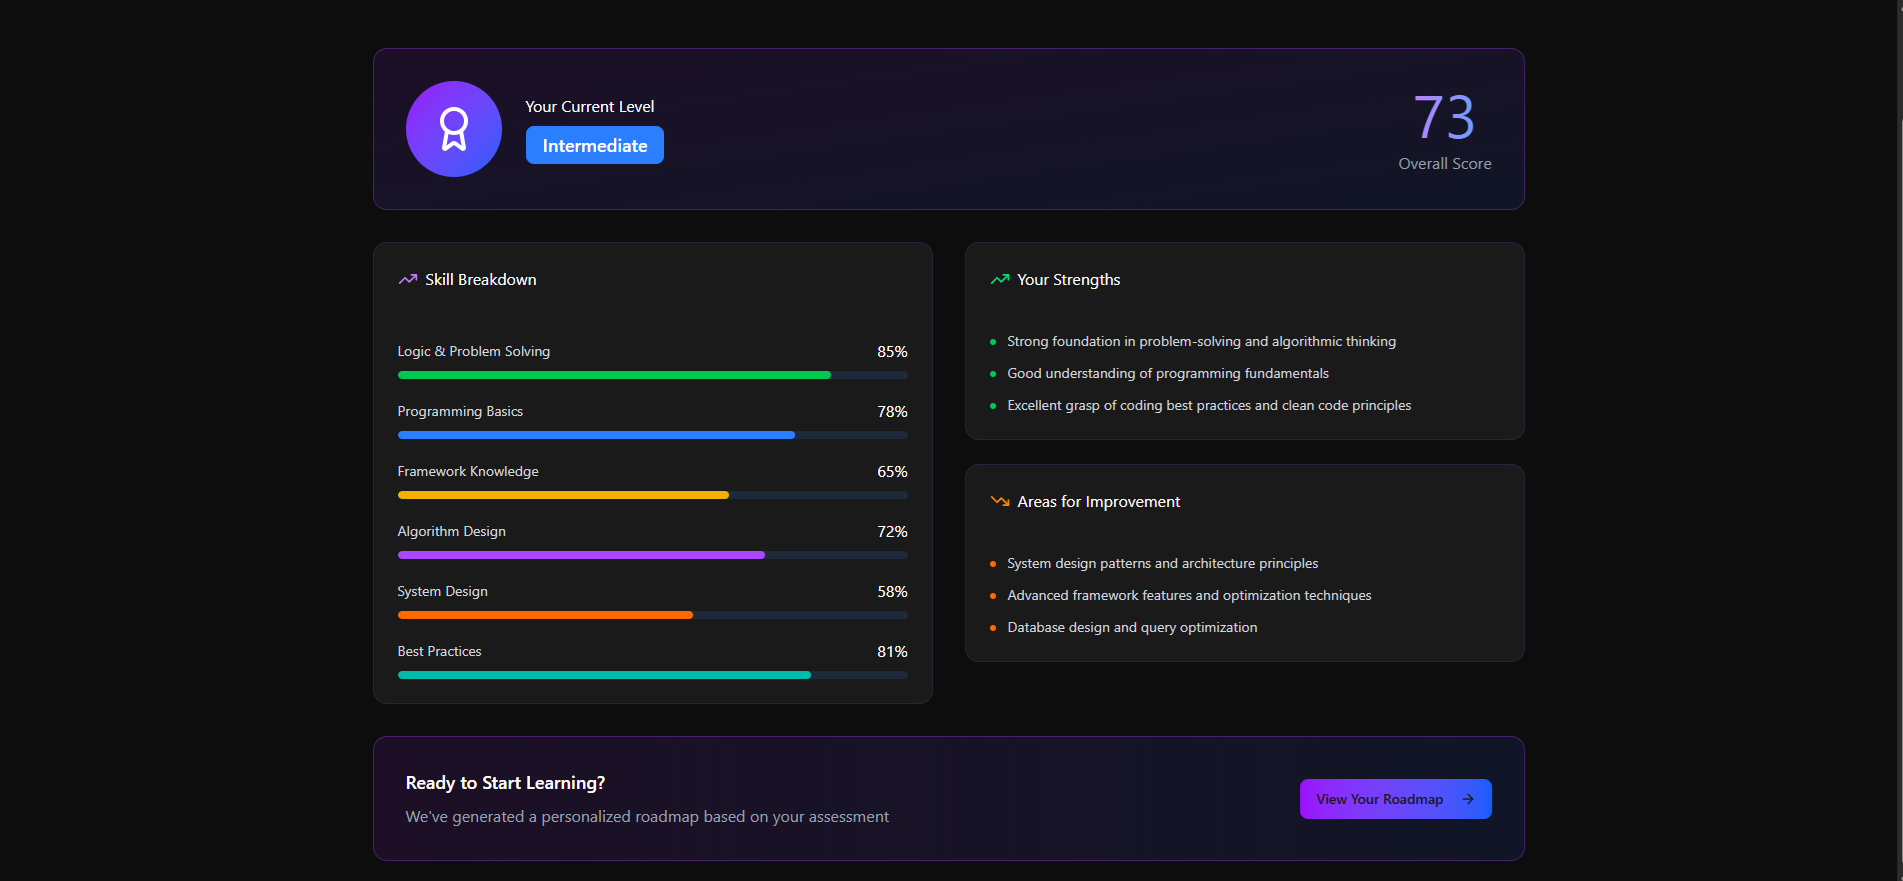
\includegraphics[width=0.9\textwidth]{Figures/Assesment report.png}
    \caption{Dashboard showing the assessment report and progress overview.}
    \label{fig:dashboard_manual}
\end{figure}

\subsection{Stat Cards}
At the top of the Dashboard, four summary cards are displayed:
\begin{itemize}
    \item \textbf{Assessments}: total number of assessments taken.
    \item \textbf{Latest Score}: your most recent assessment score percentage.
    \item \textbf{Learning Completion}: percentage of your current learning path completed.
    \item \textbf{Learning Time}: total hours spent learning.
\end{itemize}

\subsection{Activity Timeline}
Below the stat cards, an activity chart shows your learning activity over the selected time window (Last 7, 30, or 90 days). Use the \textbf{dropdown} in the top bar to switch between time windows. Click the \textbf{Refresh} icon to reload all dashboard data.

\subsection{Assessment History and AI Report}
\begin{enumerate}
    \item The left column lists all your past assessment sessions by date and track.
    \item Click any row to load the \textbf{AI Assessment Report} for that session on the right side.
    \item The report shows: executive summary, overall assessment, dimension scores, and learning priorities.
    \item At the bottom of the report, click \textbf{Continue Learning} to open your personalised learning path.
\end{enumerate}

\subsection{Comparing Two Assessments}
\begin{enumerate}
    \item In the assessment history list, tick the \textbf{checkbox} on two different sessions.
    \item The \textbf{Compare Selected} button (above the list) becomes active.
    \item Click \textbf{Compare Selected} to open a modal showing a side-by-side comparison of the two attempts.
    \item Close the modal by clicking the \textbf{X} button.
\end{enumerate}

\subsection{Path Completion Banner}
When your full learning path is complete, a banner appears at the top of the Dashboard with:
\begin{itemize}
    \item A snippet of your completion report.
    \item \textbf{Progress Analysis}: navigates to your Improvement Analysis page.
    \item \textbf{View Full Report}: opens the learning summary modal.
\end{itemize}

\section{Learning Path}

The Learning Path page (accessible via \textbf{Learning Path} in the left sidebar) shows your AI-generated personalised curriculum organised into stages. See Figure \ref{fig:roadmap} for the roadmap view.

\subsection{Navigating Stages}
\begin{enumerate}
    \item The left column lists all stages numbered in order (e.g., \textit{1. Introduction to APIs}, \textit{2. Backend Fundamentals}).
    \item Click any stage name to load it in the main panel.
    \item The selected stage shows its title, focus area, and a progress grid (completion \%, items done, time spent).
\end{enumerate}

\subsection{Generating Stage Content}
When a stage has no content yet:
\begin{enumerate}
    \item A \textbf{Generate Content} button or \textbf{Generate Stage Content} prompt will appear in the stage panel.
    \item Click it. The system will use AI with live search grounding to create 8 structured content items for that stage.
    \item Wait for the content to load (this may take a few seconds as AI generates it).
    \item Each content item shows: title, description, type (video / text / interactive), difficulty, estimated duration, and a reading/viewing body.
    \item Some items include an \textbf{Open resource} link. Click it to open the external learning resource in a new tab.
\end{enumerate}

As shown in Figure \ref{fig:module_rag}, the learning module displays AI-generated content alongside the mentor chat.

\subsection{Tracking Your Progress}
For each content item in a stage:
\begin{enumerate}
    \item A \textbf{progress strip} at the bottom shows your current status: \textit{Not started}, \textit{X\% complete}, or \textit{Completed}.
    \item If not started, click \textbf{Start Tracking} to begin timing your session.
    \item If in progress, use:
        \begin{itemize}
            \item \textbf{Update (+25\%, +10m)}: logs 25\% more completion and 10 additional minutes.
            \item \textbf{Mark Complete}: sets the item to 100\% complete.
        \end{itemize}
    \item Once all content items in all stages are marked complete, a \textbf{completion banner} appears at the top of the page.
\end{enumerate}

\subsection{Using the AI Mentor Chat}
The right column on the Learning Path page contains the \textbf{AI Mentor Chat}. This is your context-aware AI assistant for the current stage.

\begin{enumerate}
    \item Type your question about the current topic in the text field at the bottom of the chat.
    \item Press \textbf{Enter} or click \textbf{Send} to submit your question.
    \item The AI Mentor will search the knowledge base (RAG system) for relevant content and respond with a context-aware answer.
    \item Previous messages are shown in the chat history above.
    \item If the mentor is responding, a \textit{"Mentor is responding\ldots"} indicator appears.
\end{enumerate}

\noindent\textbf{Tips:}
\begin{itemize}
    \item Ask specific questions about the topics in the current stage for the best answers.
    \item If the RAG system is temporarily unavailable, the mentor will still respond using its base AI knowledge.
\end{itemize}

\subsection{Completing the Learning Path}

When all stages and content items are done:
\begin{enumerate}
    \item A completion banner appears at the top of the Learning Path page.
    \item Click \textbf{View Learning Report} to open a modal summarising your full learning journey.
    \item Click \textbf{View Progress Analysis} to navigate to your Improvement Analysis page.
    \item Click \textbf{Start AI Evaluation} to begin the AI Validator Interview and get a job-readiness score.
\end{enumerate}

\section{AI Evaluation (Validator Interview)}

The AI Evaluation module, accessible via \textbf{Real-World Validator} in the left sidebar, conducts a structured AI interview to assess your reasoning, problem-solving ability, and job readiness. See Figure \ref{fig:ai_engineer}.

\subsection{Starting a New Session}
\begin{enumerate}
    \item On the Validator page, locate the \textbf{Start New Session} panel on the right sidebar.
    \item Enter your \textbf{Path ID} (numeric; you can find this in your learning path URL or be directed here automatically from the learning path completion banner).
    \item Click \textbf{Create Session}. The AI will prepare an introductory question based on your full track and learning context.
    \item The session status badge will update once the session is ready.
\end{enumerate}

\noindent\textbf{Note:} If you navigated here by clicking \textbf{Start AI Evaluation} from the Learning Path page, the session is created automatically using your current path ID.

\subsection{Conducting the AI Interview}
\begin{enumerate}
    \item The AI Mentor opens with an introductory question displayed in the chat window (left side).
    \item Read the question carefully, then type your response in the \textbf{Your answer} text area.
    \item Press \textbf{Enter} or click \textbf{Send} to submit your response (use Shift+Enter for a new line without submitting).
    \item The AI will analyse your answer and ask follow-up questions to probe your understanding further.
    \item Continue answering. You must complete at least \textbf{3 dialogue turns} before you can end the evaluation.
    \item A hint at the bottom of the chat reminds you of the minimum dialogue requirement.
\end{enumerate}

\subsection{Completing the Evaluation}
\begin{enumerate}
    \item Once you have completed at least 3 dialogue turns, the \textbf{Complete Evaluation} button (in the right sidebar under \textbf{Evaluation Result}) becomes active.
    \item Click \textbf{Complete Evaluation}. The AI will analyse your full conversation and generate a scored report.
    \item The evaluation result panel will display:
        \begin{itemize}
            \item \textbf{Reasoning score}: how logically you approached problems.
            \item \textbf{Problem-solving score}: quality of your solutions.
            \item \textbf{Job readiness level}: overall readiness rating.
            \item \textbf{AI feedback}: written narrative of your performance.
        \end{itemize}
    \item Click \textbf{View Full Report} to open the full Evaluation Report page.
    \item Click \textbf{View Progress Analysis} to navigate to the Improvement Analysis page.
\end{enumerate}

\section{Evaluation Report}

The Evaluation Report page (\texttt{/evaluation/\{id\}}) displays the complete results of a specific evaluation session.

\begin{enumerate}
    \item The page loads automatically after evaluation completion, or you can access it via \textbf{View Full Report} from the Validator.
    \item The report shows:
        \begin{itemize}
            \item Session and path identifiers, and the date of evaluation.
            \item \textbf{Reasoning}, \textbf{Problem Solving}, and \textbf{Readiness} metric scores.
            \item \textbf{AI Feedback}: a detailed written evaluation of your performance.
            \item \textbf{Full Conversation}: the complete transcript of your AI interview session.
        \end{itemize}
    \item Click \textbf{Back to Validator} to return to the Validator page.
    \item Click \textbf{View Progress Analysis} to see your full improvement journey.
\end{enumerate}

\section{Improvement Analysis}

The Improvement Analysis page (\texttt{/improvement/\{pathId\}}) shows a comprehensive before-and-after comparison of your skills across the entire learning journey.

\begin{enumerate}
    \item Access it via \textbf{Progress Analysis} on the Dashboard, the Completion Banner on the Learning Path, or the Validator page.
    \item The page loads your full progress data. It displays:
        \begin{itemize}
            \item An \textbf{AI evaluation summary} banner at the top.
            \item A \textbf{metrics grid} showing key performance numbers.
            \item \textbf{Charts} (before vs after comparison graphs).
            \item A \textbf{story timeline} of your learning journey.
            \item \textbf{Before} and \textbf{After} skill columns: scores, levels, and optionally expandable initial assessment answers (\textbf{Show/Hide} toggle).
            \item \textbf{Improvement percentage} in the middle column where applicable.
            \item A \textbf{Detailed Progress Analysis} written report (AI-generated).
            \item \textbf{Full Interview Transcript}: click the \textbf{Show} button to expand the complete evaluation conversation.
        \end{itemize}
    \item At the bottom:
        \begin{itemize}
            \item Click \textbf{Back to Learning Path} to return to \texttt{/course}.
            \item Click \textbf{Start New Evaluation} to navigate to \texttt{/validator} and run another interview.
        \end{itemize}
\end{enumerate}

As shown in Figures \ref{fig:insights} and \ref{fig:insight2}, the insights dashboard provides a rich visual view of your learning progress.

\section{Account and Security Settings}

The Account \& Security page (\texttt{/account}) is accessible from the left sidebar under \textbf{Account \& Security}.

\subsection{Updating Your Profile}
\begin{enumerate}
    \item The page loads your current \textbf{Full Name} and \textbf{Email}.
    \item Edit either field as needed.
    \item Click \textbf{Save profile}.
    \item A success message \textit{"Profile updated successfully."} appears below the button on success.
\end{enumerate}

\subsection{Changing Your Password}
\begin{enumerate}
    \item In the \textbf{Change Password} section, enter your \textbf{Current password}.
    \item Enter a \textbf{New password} (minimum 8 characters).
    \item Re-enter the same new password in \textbf{Confirm new password}.
    \item Click \textbf{Update password}.
    \item On success, the fields are cleared and \textit{"Password changed successfully."} is shown.
\end{enumerate}

\subsection{Managing Active Sessions}
The \textbf{Active Sessions} section lists all devices currently logged into your account.

\begin{itemize}
    \item Each session shows: session ID (truncated), device/browser info, IP address, and last activity.
    \item Your current session is marked with a \textbf{Current} badge.
    \item Click \textbf{Revoke} on any session to log it out remotely.
    \item Click \textbf{Revoke Others} to log out all other devices (a confirmation dialog will appear).
    \item Click \textbf{Revoke All} to log out every session, including the current one. You will be redirected to the Home page.
    \item Click \textbf{Refresh} to reload the session list.
\end{itemize}

\subsection{Deleting Your Account}
\textbf{Warning: This action is permanent and cannot be undone.}

\begin{enumerate}
    \item Scroll to the \textbf{Delete Account} section.
    \item Type the word \textbf{DELETE} (case-insensitive) in the confirmation field.
    \item Click \textbf{Delete my account}.
    \item A second browser confirmation dialog will appear. Click \textbf{OK} to confirm.
    \item Your account and all data are permanently deleted. You will be redirected to the Home page.
\end{enumerate}

\section{Logging Out}

To log out of GrowWise:

\begin{enumerate}
    \item Open the \textbf{Account \& Security} page from the left sidebar.
    \item In the \textbf{Active Sessions} section, locate the session marked \textbf{Current}.
    \item Click \textbf{Log Out This Device}.
    \item You will be redirected to the Home page and the session will be terminated.
\end{enumerate}

Alternatively, you can log out all devices at once by clicking \textbf{Revoke All} in the Active Sessions section.

\section{Conclusion}

This chapter provided a complete walkthrough of the GrowWise platform. A new user can follow these steps in sequence: Sign Up, Log In, Select a Track, Complete the Assessment, follow the personalised Learning Path, use the AI Mentor Chat, complete the AI Evaluation, and review their Improvement Analysis. This covers the full learning cycle from start to finish. The platform is designed to be self-explanatory, with clear guidance at every step to ensure learners can progress without confusion.


\chapter{Conclusions}
\section{Project Summary and Achievements}
The final project is the construction of GrowWise, an AI-enhanced adaptive learning platform, which seals huge gaps in the way developers learn. It struck the overall target of creating a personalized system centered on approaches, and passing the outdated fixed courses to deliver vibrant, conscious education tailored to each individual. In examining fifteen other platforms we identified such weaknesses as lack of real-time checks on structure, minimal emphasis on problem solving, and complete AI mentoring. The fix consists of Next.js, FastAPI, PostgreSQL, and AI API as the tools of a scalable and simple to maintain platform that develops skills and thought processes.
\section{Key Findings and Results}
The review demonstrated that others excel in areas such as projects (freeCodeCamp, Udacity), adaptive tests (Pluralsight, DataCamp), and AI (CYPHER Learning), but none of them combine it in the way GrowWise does. The arrangement closes the gaps with on-the-fly routes, real-time assistance with AI through RAG pulls, and complete abilities and logic examination. The modular construction allows parting work and tests, and the additions and amendments are not difficult. The complete documentation containing diagrams, interactions and plans provide proper building and rollout.
\section{Project Scope Coverage and Objectives Achievement}
We went through it all and achieved all objectives. The design manages users, path making, AI tests and tracking where necessary. It accompanies tracks, provides personal experiences and has user and admin views. All the needs concerning functionalities, performance, security, scale, and convenience are addressed. It is a combination of a method-based approach to learning and AI assistance, forming a new platform between school and work. Our fix was to the extent of what is allowed to ensure that developer learning issues were full.
\section{Challenges Faced and Limitations}
We hit some hurdles. Combining AI services and maintaining speed required special consideration and adjustments. Responsive design and backups were required to make it work well on devices and networks. The dynamic nature of AI content required powerful error corrections. Constant adjustments were balancing between deep checks and speed. There are limitations such as the use of external AI, which might compromise the uptime and speed. It has gone web based and thus not much on mobile enthusiasts. Besides, its effectiveness is determined by the quality of materials and knowledge base.
\section{Long-term Recommendations}
In more detail, the following ideas can be noted:
\begin{itemize}
\item Mobile Application Development: Add iOS and Android applications to access it and have fun even better.
\item Advanced AI Capabilities: Have finer AI run code checks, structure reviews, and custom tips that are oriented at learning the language.
\item Community Features: Have peer reviews, forums and projects that are undertaken in groups.
\item Industry Integration: Collaborate with companies in actual projects and mentoring.
\item Advanced Analytics: Develop insights using predictions, gap forecasts, and general measures to keep improving.
\item Multi-language Support: Support additional languages and structures to access additional developers.
\item Enterprise Features: Custom paths and make team tools and tracking for companies and schools.
\end{itemize}
\section{Final Remarks}
GrowWise will contribute significantly to the developer education, sealing discontinuities with novel AI and emphasis on methods. The concrete construction and build strategy prepares a platform-altering platform that accommodates dynamically evolving technology. It demonstrates the ability of AI personal learning technology to transform technological learning, providing a scalable solution to students, institutions, and enterprises. The FYP-2 plan continues the momentum on a complete platform that improves the developer skills in the modern world.

% ---------- References ----------
\renewcommand{\bibname}{References}
\cleardoublepage
\addcontentsline{toc}{chapter}{References}
\bibliographystyle{IEEEtran}
\bibliography{fypbib}

% ---------- Appendices (optional) ----------
\appendix

\end{document}


